\documentclass[a4paper,13pt]{report}
\usepackage[utf8]{vietnam}
\usepackage[utf8]{inputenc}
\usepackage{amsmath}
\usepackage{amsfonts}
\usepackage{amssymb}
\usepackage{graphicx}
\usepackage{xspace}
\usepackage{caption}
\usepackage{array}
\usepackage[font=small]{caption}
\usepackage{booktabs}
\usepackage{tabularx}
\usepackage{ragged2e}
\usepackage[unicode]{hyperref}
\usepackage[left=3cm,right=2cm,top=2.5cm,bottom=3cm]{geometry}
\usepackage{titlesec}
\usepackage{scrextend}
\usepackage{enumerate}
\usepackage{url}
\usepackage{tikz}
\usepackage{float}
\usepackage{afterpage}
\usepackage{multirow}
\usepackage{sectsty}
\usepackage{longtable}
\usepackage{tocloft,calc}
\usepackage{makecell}
\usepackage[square,sort,comma,numbers]{natbib}
\usepackage{natbib}
\usepackage{algorithm}
\usepackage{subcaption}
\usepackage{minted}
\usepackage{listings}
\usepackage{xcolor}
\usetikzlibrary{calc}
% \usepackage[perpage]{footmisc}
\usepackage[flushleft]{threeparttable}
% \usepackage{subcaption}
\usepackage{perpage} %the perpage package
\MakePerPage{footnote} %the perpage package command
% \usepackage[ruled,vlined]{algorithm2e}
\PassOptionsToPackage{table}{xcolor}

\def\changemargin#1#2{\list{}{\rightmargin#2\leftmargin#1}\item[]}
\let\endchangemargin=\endlist

\changefontsizes{13pt}

\makeatletter
\def\l@figure{\@dottedtocline{1}{1em}{2.2em}}
\def\l@table{\@dottedtocline{1}{1em}{2.2em}}
\renewcommand*{\ALG@name}{Thuật toán}
\makeatother

\sectionfont{\fontsize{15}{15}\selectfont}
\subsectionfont{\fontsize{13}{15}\selectfont}

\titleformat{\chapter}[display]
{\normalfont\huge\bfseries}{\chaptertitlename\ \thechapter}{0pt}{\LARGE}
\titlespacing*{\chapter}{0cm}{-\topskip}{0pt}[0pt]

\titleclass{\subsubsubsection}{straight}[\subsection]

\newcounter{subsubsubsection}[subsubsection]
\renewcommand\thesubsubsubsection{\thesubsubsection.\arabic{subsubsubsection}}
\renewcommand\theparagraph{\thesubsubsubsection.\arabic{paragraph}} % optional; useful if paragraphs are to be numbered

\titleformat{\subsubsubsection}
  {\normalfont\normalsize\bfseries}{\thesubsubsubsection}{1em}{}
\titlespacing*{\subsubsubsection}
{0pt}{3.25ex plus 1ex minus .2ex}{1.5ex plus .2ex}
\def\toclevel@subsubsubsection{4}
\def\l@subsubsubsection{\@dottedtocline{4}{7em}{4em}}

\renewcommand{\baselinestretch}{1.3}
%\renewcommand{\cftsecpresnum}{Chương\space}
\renewcommand{\cftchappresnum}{Chương }
\AtBeginDocument{\addtolength\cftchapnumwidth{\widthof{\bfseries Chương }}}
\setlength{\parskip}{0.4em}
\setlength{\parindent}{0pt}
%
\title{Xây dựng công cụ phân tích mã nguồn cho ngôn ngữ Rust}	%% title
\author{Công Nghĩa Hiếu}			%% author's name

%
\newcommand{\argmax}{\arg\!\max}
\newcommand{\tool}{\textsc{DeFP}\xspace}
\newcommand{\toolLong}{\textbf{De}tect \textbf{F}alse \textbf{P}ositive\xspace}

\definecolor{dkgreen}{rgb}{0,0.6,0}
\definecolor{gray}{rgb}{0.5,0.5,0.5}
\definecolor{mauve}{rgb}{0.58,0,0.82}
\definecolor{gray}{rgb}{0.4,0.4,0.4}
\definecolor{darkblue}{rgb}{0.0,0.0,0.6}
\definecolor{lightblue}{rgb}{0.0,0.0,0.9}
\definecolor{cyan}{rgb}{0.0,0.6,0.6}
\definecolor{darkred}{rgb}{0.6,0.0,0.0}
\definecolor{bg_gray}{RGB}{242, 242, 235}

\renewcommand{\lstlistingname}{Hình}
\newcommand{\cev}[1]{\reflectbox{\ensuremath{\vec{\reflectbox{\ensuremath{#1}}}}}}



\lstset{
  basicstyle=\ttfamily\footnotesize,
  columns=fullflexible,
  showstringspaces=false,
  numbers=left,                   % where to put the line-numbers
  numberstyle=\small\color{gray},  % the style that is used for the line-numbers
  stepnumber=1,
  numbersep=5pt,                  % how far the line-numbers are from the code
  backgroundcolor=\color{bg_gray},      % choose the background color. You must add \usepackage{color}
  showspaces=false,               % show spaces adding particular underscores
  showstringspaces=false,         % underline spaces within strings
  showtabs=false,                 % show tabs within strings adding particular underscores
  frame=none,                   % adds a frame around the code
  rulecolor=\color{black},        % if not set, the frame-color may be changed on line-breaks within not-black text (e.g. commens (green here))
  tabsize=2,                      % sets default tabsize to 2 spaces
  captionpos=b,                   % sets the caption-position to bottom
  breaklines=true,                % sets automatic line breaking
  breakatwhitespace=false,        % sets if automatic breaks should only happen at whitespace
  title=\lstname,                   % show the filename of files included with \lstinputlisting;
                                  % also try caption instead of title
  commentstyle=\color{gray}\upshape
}


\lstdefinelanguage{XML}
{
  morestring=[s][\color{mauve}]{"}{"},
  morestring=[s][\color{black}]{>}{<},
  morecomment=[s]{<?}{?>},
  morecomment=[s][\color{dkgreen}]{<!--}{-->},
  stringstyle=\color{black},
  identifierstyle=\color{lightblue},
  keywordstyle=\color{red},
  morekeywords={xmlns,xsi,noNamespaceSchemaLocation,type,id,x,y,source,target,version,tool,transRef,roleRef,objective,eventually}% list your attributes here
}

\definecolor{codegreen}{rgb}{0,0.6,0}
\definecolor{codegray}{rgb}{0.5,0.5,0.5}
\definecolor{codepurple}{rgb}{0.58,0,0.82}
\definecolor{backcolour}{rgb}{0.95,0.95,0.92}

\begin{document}
% Cover Vietnamese 1

% Cover Vietnamese 1

% Cover english
\pagenumbering{gobble}
\begin{center}
	\begin{tikzpicture}[overlay,remember picture]
	    \draw [line width=3pt,rounded corners=0pt,
	        ]
	        ($ (current page.north west) + (25mm,-25mm) $)
	        rectangle
	        ($ (current page.south east) + (-15mm,25mm) $);
	    \draw [line width=1pt,rounded corners=0pt]
	        ($ (current page.north west) + (26.5mm,-26.5mm) $)
	        rectangle
	        ($ (current page.south east) + (-16.5mm,26.5mm) $);
	\end{tikzpicture}
	\\[1mm]
	%%12pt
	\textbf{ĐẠI HỌC QUỐC GIA HÀ NỘI\\TRƯỜNG ĐẠI HỌC CÔNG NGHỆ}\\[1cm]
	
\includegraphics[width=0.2\linewidth]{figures/uet}\\[0.3cm]
	\textbf{Công Nghĩa Hiếu}
	\\[2cm]

	\large{\textbf{XÂY DỰNG CÔNG CỤ PHÂN TÍCH MÃ NGUỒN CHO NGÔN NGỮ RUST}}
	\\[2.6cm]
	\normalsize{\textbf{KHOÁ LUẬN TỐT NGHIỆP ĐẠI HỌC HỆ CHÍNH QUY
		\\[2mm]
	Ngành: Công nghệ thông tin}}

	\vfill
	\textbf{HÀ NỘI - 2024}
	\vspace{10mm}
\end{center}

\begin{center}

	
\begin{tikzpicture}[overlay,remember picture]
	\draw [line width=3pt,rounded corners=0pt,
	]
	($ (current page.north west) + (25mm,-25mm) $)
	rectangle
	($ (current page.south east) + (-15mm,25mm) $);
	\draw [line width=1pt,rounded corners=0pt]
	($ (current page.north west) + (26.5mm,-26.5mm) $)
	rectangle
	($ (current page.south east) + (-16.5mm,26.5mm) $);
	\end{tikzpicture}
	\\[1mm]
	\textbf{ĐẠI HỌC QUỐC GIA HÀ NỘI\\TRƯỜNG ĐẠI HỌC CÔNG NGHỆ}
	\\[1cm]
	
\includegraphics[width=0.2\linewidth]{figures/uet}
	\\[0.3cm]
	\textbf{Công Nghĩa Hiếu}
	\\[2cm]

	\large{\textbf{XÂY DỰNG CÔNG CỤ PHÂN TÍCH MÃ NGUỒN CHO NGÔN NGỮ RUST}}
	\\[2.6cm]
	\normalsize{\textbf{KHOÁ LUẬN TỐT NGHIỆP ĐẠI HỌC HỆ CHÍNH QUY
		\\[2mm]
	Ngành: Công nghệ thông tin}}
\end{center}
\vspace{16mm}
\hspace*{12mm}\textbf{Cán bộ hướng dẫn: PGS. TS. Võ Đình Hiếu}\\[0.8cm]

\vfill
\begin{center}
	\textbf{HÀ NỘI - 2024}
	\vspace{10mm}
\end{center}


\begin{center}

	
\begin{tikzpicture}[overlay,remember picture]
	\draw [line width=3pt,rounded corners=0pt,
	]
	($ (current page.north west) + (25mm,-25mm) $)
	rectangle
	($ (current page.south east) + (-15mm,25mm) $);
	\draw [line width=1pt,rounded corners=0pt]
	($ (current page.north west) + (26.5mm,-26.5mm) $)
	rectangle
	($ (current page.south east) + (-16.5mm,26.5mm) $);
	\end{tikzpicture}
	\\[1mm]
	\textbf{ VIETNAM NATIONAL UNIVERSITY, HANOI\\UNIVERSITY OF ENGINEERING AND TECHNOLOGY}
	\\[1cm]
	
\includegraphics[width=0.2\linewidth]{figures/uet}
	\\[0.3cm]
	\textbf{Cong Nghia Hieu}
	\\[2cm]

	\textbf{DEVELOPING A SOURCE CODE ANALYSIS TOOL FOR THE RUST PROGRAMMING LANGUAGE}
	\\[2.6cm]
	\textbf{BACHELOR'S THESIS
		\\[2mm]
		Major: Information technology}
\end{center}
\vspace{16mm}
\hspace*{12mm}\textbf{ Supervisor: Assoc. Prof., Dr. Vo Dinh Hieu}\\[0.8cm]

\vfill
\begin{center}
	\textbf{HANOI - 2024}
	\vspace{4mm}
\end{center}

\newpage\cleardoublepage

% Acknowledgement
\begin{center}
\textbf{\large{Lời cảm ơn}	}
\end{center}
\addcontentsline{toc}{chapter}{Lời cảm ơn}

Lời đầu tiên, tôi xin bày tỏ lòng biết ơn sâu sắc tới thầy Võ Đình Hiếu, người đã tận tình chỉ bảo tôi trong suốt quá trình học tập tại trường và đặc biệt là thời gian thực hiện khóa luận tốt nghiệp.
Thầy đã không chỉ cung cấp những chỉ dẫn chuyên môn mà còn động viên và hỗ trợ tôi vượt qua khó khăn để thực hiện đề tài tốt nghiệp một cách tốt nhất.

Tôi cũng xin cảm ơn thầy Trần Mạnh Cường và thầy Vũ Trọng Thanh cũng như toàn thể anh chị, và các bạn trong phòng thí nghiệm iSE (Khoa Công nghệ thông tin, Trường Đại học Công nghệ, ĐHQGHN) đã ủng hộ động viên tôi trong quá trình hoàn thành khóa luận.
Sự hỗ trợ nhiệt tình của mọi người đã giúp tôi có thêm tự tin trong việc mở rộng kiến thức và kỹ năng thực hành.

Chúc mọi người luôn vui vẻ và gặt hái được nhiều thành công trong cuộc sống.

\newpage\cleardoublepage
% Assurance
\setcounter{page}{1}
\pagenumbering{roman}
\begin{center}
\textbf{\large{Lời cam đoan}	}
\end{center}
\addcontentsline{toc}{chapter}{Lời cam đoan}

Tôi là Công Nghĩa Hiếu, sinh viên lớp QH-2021-I/CQ-I-IT2 khóa K66 theo học ngành Công nghệ thông tin tại trường Đại học Công Nghệ - Đại học Quốc gia Hà Nội.
Tôi xin cam đoan khoá luận "Xây dựng công cụ phân tích mã nguồn cho ngôn ngữ Rust" là công trình nghiên cứu do bản thân tôi thực hiện.
Các nội dung nghiên cứu, kết quả trong khoá luận là xác thực.

Các thông tin sử dụng trong khoá luận là có cơ sở và không có nội dung nào sao chép từ các tài liệu mà không ghi rõ trích dẫn tham khảo.
Tôi xin chịu trách nhiệm về lời cam đoan này.

\begin{flushright}
Hà Nội, ngày 16 tháng 12 năm 2024
\end{flushright}

\begin{changemargin}{11.5cm}{2cm}
Sinh viên
\\[2cm]
\end{changemargin}

\begin{changemargin}{11cm}{2cm}
Công Nghĩa Hiếu
\end{changemargin}\newpage\cleardoublepage
% Abstract Vietnamese
\begin{center}
\textbf{\large{Tóm tắt}	}
\end{center}

\addcontentsline{toc}{chapter}{Tóm tắt}

\begin{small}
Với sự phát triển mạnh mẽ của API, kiểm thử  API là một chủ đề được quan tâm đặc biệt trong lĩnh vực nghiên cứu hiện nay, bởi vì API đóng vai trò quan trọng trong việc kết nối các hệ thống và ứng dụng. Đi cùng sự phát triển nhanh chóng của công nghệ và nhu cầu tích hợp liên tục, việc đảm bảo chất lượng và hiệu suất của các API trở nên cấp thiết.

Khóa luận này đã trình bày công cụ kiểm thử tự động API ứng dụng học tăng cường với một phương pháp đánh giá điểm thưởng tập trung vào việc tối ưu hóa mức độ phủ trong kiểm thử API, đảm bảo tính hiệu quả và toàn diện trong quá trình đánh giá. 
Qua quá trình thực nghiệm trên một tập các dịch vụ kiểm thử  uy tín, kết quả cho thấy công cụ được phát triển có thể xác định được 126,9 lỗi riêng biệt với mã trả về dạng \texttt{500}, vượt trội hơn 14 lỗi so với ARAT-RL, công cụ kiểm thử tự động API mới nhất hiện nay \cite{kim2023adaptive}. Về tốc độ, tại đa số thời điểm, công cụ được trình bày đều cho thấy hiệu suất tốt hơn so ARAT-RL. Đặc biệt, tại một số thời điểm, trên cùng một mốc yêu cầu, công cụ này vượt trội hơn với 15 lỗi tìm được nhiều hơn. Những kết quả này chứng minh rằng công cụ không chỉ cải thiện về mặt số lượng lỗi phát hiện được mà còn tăng tốc độ phát hiện lỗi, giúp tiết kiệm tài nguyên và nâng cao chất lượng phần mềm.


\vspace*{1cm}
\textbf{Từ khóa}: Phân tích mã nguồn, phân tích tĩnh, ngôn ngữ lập trình Rust

\end{small}\newpage\cleardoublepage
% Abstract English
\begin{center}
\textbf{\large{Abstract}	}
\end{center}

\addcontentsline{toc}{chapter}{Abstract}
\begin{small}

With the rapid development of APIs, API testing has become a topic of particular interest in current research because APIs play a crucial role in connecting systems and applications. As technology evolves and the need for continuous integration grows, ensuring the quality and performance of APIs becomes essential.

This thesis presents an automated API testing tool that employs reinforcement learning with a reward evaluation method focused on optimizing test coverage, ensuring efficiency and comprehensiveness in the evaluation process. Through experiments on reputable testing services, the results demonstrate that the developed tool can identify 126.9 distinct errors with a 500 response code, surpassing ARAT-RL, the latest automated API testing tool, by 14 errors. In terms of speed, the presented tool generally shows better performance than ARAT-RL. Notably, at certain points, on the same request milestone, this tool outperforms with 15 more errors detected. These results prove that the tool not only improves the number of detected errors but also increases the speed of error detection, saving resources and enhancing software quality.



\vspace*{1cm}
\textbf{Keywords}: Source code analysis, static analysis, Rust programming language
\end{small}\newpage\cleardoublepage
\addcontentsline{toc}{chapter}{Mục lục}
\tableofcontents\newpage\cleardoublepage
%

\newpage
\addcontentsline{toc}{chapter}{\listfigurename}
\listoffigures\cleardoublepage

\newpage
\addcontentsline{toc}{chapter}{\listtablename}
\listoftables

\newpage
\chapter*{Danh mục từ viết tắt}
\addcontentsline{toc}{chapter}{Danh mục từ viết tắt}

% \begin{table}[h]
% \begin{tabularx}{\textwidth}{|l|l|X|X|}
% \hline
% \textbf{STT} & \textbf{Từ viết tắt} &  \textbf{Cụm từ đầy đủ} & \textbf{Cụm từ tiếng Việt} \\
% \hline
% 1 & AST & Abstract Syntax Tree & Cây cú pháp trừu tượng \\
% \hline
% 2 & CFG & Control Flow Graph & đồ thị CFG \\
% \hline
% 3 & PDG & Program Dependence Graph & Đồ thị phụ thuộc chương trình \\
% \hline
% 4 & CDG & Control Dependence Graph & Đồ thị phụ thuộc điều khiển \\
% \hline
% 5 & CPG & Code Property Graph & Đồ thị thuộc tính mã nguồn \\
% \hline
% 6 & IDE & Integrated Development Environment & Môi trường phát triển tích hợp \\
% \hline
% \end{tabularx}
% \end{table}

\begin{table}[h]
\begin{tabularx}{\textwidth}{|l|l|X|X|}
\hline
\textbf{Từ viết tắt} & \textbf{Cụm từ đầy đủ} & \textbf{Cụm từ tiếng Việt} \\
\hline
AST & Abstract Syntax Tree & Cây cú pháp trừu tượng \\
\hline
CFG & Control Flow Graph & đồ thị CFG \\
\hline
PDG & Program Dependence Graph & Đồ thị phụ thuộc chương trình \\
\hline
% CDG & Control Dependence Graph & Đồ thị phụ thuộc điều khiển \\
% \hline
CPG & Code Property Graph & Đồ thị thuộc tính mã nguồn \\
\hline
% IDE & Integrated Development Environment & Môi trường phát triển tích hợp \\
% \hline
JSON & JavaScript Object Notation & Ký hiệu đối tượng JavaScript \\
\hline
XML & Extensible Markup Language & Ngôn ngữ đánh dấu mở rộng \\
\hline
YAML & YAML Ain't Markup Language & Ngôn ngữ đánh dấu YAML \\
\hline
OOP & Object-Oriented Programming & Lập trình hướng đối tượng \\
\hline
FP & Functional Programming & Lập trình hướng hàm \\
\hline
DSL & Domain-Specific Language & Ngôn ngữ miền chuyên biệt \\
\hline
%  & Ownership & Sở hữu giá trị \\
% \hline
%  & Borrow & Mượn giá trị \\
% \hline
%  & Lifetime & Vòng đời giá trị \\
% \hline
% & Thread & Luồng  \\
% \hline
\end{tabularx}
\end{table}\newpage\cleardoublepage
% \listoftables

\setcounter{page}{1}
\pagenumbering{arabic}

% \chapter*{Mở đầu}
\setcounter{page}{1}
\pagenumbering{arabic}
Trong thời đại mà những đổi mới về mặt công nghệ đang định hình lại thế giới, nhiều khía cạnh trong cuộc sống hàng ngày của con người đang chuyển dần sang những nền tảng ảo. Mô hình của các nền tảng này hướng đến khả năng kết nối và trao đổi thông tin giữa nhiều thiết bị công nghệ giúp tối ưu hóa sự tiện nghi cho con người, tuy nhiên từ đó lại đi kèm rủi ro khi dữ liệu riêng tư của người dùng được chia sẻ qua không gian mạng. Các cuộc tấn công khai thác lỗ hổng phần mềm (Software Vulnerability) nhằm vào hệ thống phần mềm máy tính, đặc biệt là các hệ thống quan trọng như quản lý dữ liệu công dân quốc gia, giao thông, điều phối hàng không, vận hành công nghiệp hóa học/hạt nhân, và các hệ thống an ninh quốc phòng, và có thể gây ra thiệt hại đáng kể. Theo khảo sát của Veracode trên hơn 130,000 phần mềm năm 2020, hơn 75\% trong số đó chứa ít nhất một lỗ hổng phần mềm~\cite{veracode}. Các lỗ hổng phổ biến bao gồm: kiểm soát truy cập bị hỏng (Broken Access Control), lỗi mật mã (Cryptographic Failures), SQL Injections, thiết kế không an toàn, cấu hình bảo mật sai. Vào năm 2021, 97\% phần mềm trong tổng số 2,409 phần mềm có chứa mã nguồn mở~\cite{synopsys}. 80\% trong số đó có chứa ít nhất một lỗ hổng phần mềm. 


Từ đó, một trong những mục tiêu quan trọng nhất của công nghệ phần mềm là làm thế nào để xây dựng phần mềm có khả năng đứng vững trước sự tấn công vào những lỗ hổng có trong phần mềm~\cite{mcgraw2006software}. Hiện nay có rất nhiều giải pháp được thiết kế nhằm giúp các nhà phát triển phần mềm xây dựng phần mềm an toàn hơn, chẳng hạn như thiết kế phần mềm theo quy chuẩn chung, kiểm thử phần mềm, nhận diện và phân tích các lỗ hổng để đánh giá tác động của những chúng lên phần mềm, và giảm độ phức tạp và tăng khả năng mở rộng của phần mềm, v.v. Ngoài ra, việc thực thi các phương pháp phân tích chương trình khác nhau trên mã nguồn phần mềm hoặc trên các phiên bản đã biên dịch có thể giúp phát hiện ra các lỗ hổng bảo mật tiềm ẩn có thể xảy ra. Nhìn chung, các phương pháp tiếp cận phân tích mã có thể được chia thành hai nhóm chính: Phân tích mã nguồn tĩnh (Static Code Analysis - SCA) và Phân tích chương trình động (Dynamic Program Analysis - DPA)~\cite{mcgraw2006software}.

Những nghiên cứu trước đây đã cho thấy DPA là một kỹ thuật hiệu quả để tìm ra các lỗi bảo mật tiềm ẩn trong mã nguồn bằng cách phân tích các hành vi của chương trình khi nó đang thực thi~\cite{andreasen2017survey}. Hơn nữa, kỹ thuật DPA có thể yêu cầu can thiệp và sửa đổi mã nguồn chương trình nhằm mục đích thu thập dấu vết trong quá trình chạy để phát hiện được những hành vi nghi vấn~\cite{larus1994rewriting}. Tuy nhiên, nhược điểm của DPA là phải chịu chi phí về mặt thời gian khi phải thực thi chương trình phức tạp. Bên cạnh đó, việc dựa vào DPA để tìm các lỗi có trong mã nguồn phần mềm có thể không còn hữu dụng khi thời điểm lỗi được phát hiện thường nằm về cuối của vòng đời phát triển phần mềm. Trái ngược với DPA, SCA xác định các lỗi tiềm ẩn trong phần mềm bằng cách phân tích mã nguồn hoặc mã nhị phân của phần mềm mà không cần thực thi~\cite{zheng2006value}. Các cảnh báo về lỗi phần mềm do các công cụ SCA tạo ra có thể được phân loại thành 3 nhóm chính: (1) \textit{dương tính giả} (False Positive - FP): là cảnh báo về lỗi nhưng thực sự thì lỗi đó không tồn tại; (2) \textit{dương tính thật} (True Positive - TP): là cảnh báo đúng về các lỗi tiềm ẩn đang nằm trong mã nguồn; (3) {âm tính giả} (False Negative - FN): là khi SCA không phát hiện ra lỗi, mặc dù thực sự lỗi có tồn tại trong mã nguồn~\cite{alikhashashneh2018using}.

Trong quá khứ đã có một số nghiên cứu tập để đánh giá chất lượng của các công cụ phân tích tĩnh (SCA Tool). Nghiên cứu của Ramos~\cite{ramos2016evaluating} đã đánh giá độ chính xác của Visual Code Grepper, FindBugs và SonarQube trong việc phát hiện các lỗ hổng SQL Injections, OS Command và LDAP Injections đối với bộ dữ liệu chuẩn Java Juliet~\cite{JULIET}. Tương tự như vậy, McLean~\cite{mclean2012comparing} đã thực hiện đánh giá một số công cụ phân tích tĩnh đối với các ứng dụng mã nguồn mở được sử dụng rộng rãi, chẳng hạn như Apache OpenOffice (AOO)~\cite{steinberg2013apache}, PuTTY~\cite{dooley2006cisco}, NMAP~\cite{lyon2008nmap} và Wireshark~\cite{orebaugh2006wireshark}. Tuy nhiên, giống như nhiều công cụ và kỹ thuật khác, công cụ phân tích tĩnh có một số nhược điểm cố hữu, trong đó nổi bật là việc SCA thường tạo ra một số lượng lớn các kết quả dương tính giả và âm tính giả. Trên thực tế, Kremenek và Engler~\cite{kremenek2003z} đã quan sát thấy rằng tỷ lệ dương tính giả đối với một số công cụ SCA nằm trong khoảng từ 30\%-100\%. Các nghiên cứu khác~\cite{boogerd2006prioritizing,heckman2008establishing} cũng đã chỉ ra rằng 35\%-91\% cảnh báo được báo cáo là dương tính giả. Theo nguyên tắc, để tránh bỏ sót lỗi có trong phần mềm thì các lập trình viên vẫn phải kiểm tra thủ công tất cả các cảnh báo đã được tạo ra để xác định chúng là cảnh báo dương tính giả hay dương tính thật. Tuy nhiên việc kiểm tra tất cả cảnh báo theo cách thủ công tiêu tốn một lượng lớn thời gian và nguồn lực, từ đó trở thành rào cản chính khiến các nhà phát triển phần mềm ngần ngại sử dụng các công cụ SCA cho các dự án của họ. Một giải pháp để giải quyết vấn đề này là thiết kế bước hậu xử lý giúp loại bỏ các cảnh báo dương tính giả một cách tự động, từ đó giữ lại được những cảnh báo có khả năng cao là dương tính thật để được đưa vào kiểm tra thủ công.

Theo định hướng đó, để giải quyết vấn đề về cảnh báo sai của các công cụ phân tích tĩnh, luận văn này sẽ trình bày một giải pháp giúp xếp hạng lại tập cảnh báo được tạo ra bởi các công cụ phân tích tĩnh. Ý tưởng chính của nghiên cứu dựa trên quan sát rằng các cảnh báo có bối cảnh tương tự thường có nhãn tương tự (TP hoặc FP). Đối với mỗi cảnh báo, giải pháp sẽ phân tích ngữ cảnh của cảnh báo cả về mặt cú pháp và ngữ nghĩa, sau đó áp dụng mô hình học sâu để dự đoán khả năng cảnh báo đó là TP (hay FP). Cụ thể, để có được ngữ cảnh của một cảnh báo, \tool áp dụng các kĩ thuật phân tích chương trình để trích xuất tất cả các câu lệnh có ảnh hưởng và bị ảnh hưởng bởi câu lệnh bị đánh dấu bởi công cụ phân tích tĩnh. Sau đó, để thể hiện giúp mô hình học được những mẫu ngữ cảnh chung, tên của các hằng số/biến số/phương thức sẽ được thay thế bằng tên trừu tượng. Tiếp theo, các câu lệnh bị cảnh báo và ngữ cảnh liên quan sẽ được véc-tơ hóa và dùng làm đầu vào để huấn luyện các mô hình mạng học sâu. Cuối cùng, các cảnh báo đầu vào sẽ được xếp hạng theo điểm dự đoán tương ứng của mô hình học sâu.

Ngoài ra, theo hiểu biết của học viên, hiện tại vẫn chưa có một bộ dữ liệu công khai nào được xây dựng trên các hệ thống phần mềm thực tế để đánh giá độ hiệu quả của các phương pháp hậu xử lý cảnh báo sai sinh ra từ các công cụ phân tích tĩnh. Trong các nghiên cứu hiện có~\cite{flynn2018prioritizing, berman2019active}, các mô hình học máy thường được đào tạo và thử nghiệm trên các bộ dữ liệu tổng hợp là Juliet~\cite{JULIET} và SARD~\cite{SARD}. Tuy nhiên, các bộ dữ liệu này đều chỉ bao gồm các ví dụ đơn giản với các lỗi được tạo ra dựa trên các mẫu lỗ hổng đã biết. Nghiên cứu của Chakraborty và cộng sự~\cite{chakraborty2021deep} cũng đã chứng minh rằng các bộ dữ liệu còn quá đơn giản và không phản ánh được hiệu suất của các cách tiếp cận khi được áp dụng trong thực tế. Vì vậy, để giải quyết hạn chế thiếu hụt dữ liệu, luận văn này còn đóng góp một bộ dữ liệu chứa 6,620 cảnh báo của 10 dự án phần mềm mã nguồn mở.

Về kết quả thực nghiệm, giải pháp \tool cho thấy rằng khoảng 60\% lỗ hổng thực tế được \tool xếp hạng sẽ nằm trong 20\% cảnh báo đầu tiên của danh sách. Hơn nữa, lập trình viên sử dụng \tool có thể tìm thấy hơn 90\% lỗ hổng thực tế mà chỉ cần kiểm tra 60\% tổng số cảnh báo. Trong khi đó, bằng cách sử dụng phương pháp được cho là tốt nhất hiện nay~\cite{lee2019classifying}, các lập trình viên chỉ có thể tìm thấy 46\% và 82\% số lượng cảnh báo là TP với cùng số lượng cảnh báo được kiểm tra.

Về chi tiết, luận văn sẽ được trình bày theo cấu trúc như sau. Chương 1 sẽ giới thiệu kĩ hơn về những vấn đề mà các công cụ phân tích tĩnh đang gặp phải, những nghiên cứu trước đây và đặt vấn đề cần giải quyết trong luận văn này. Chương 2 sẽ nhắc lại sơ lược một số kiến thức cơ sở về công cụ phân tích tĩnh, các kĩ thuật phân tích chương trình và mô hình học biểu diễn bằng học sâu. Giải pháp được xây dựng trong luận văn sẽ được mô tả chi tiết ở Chương 3. Tiếp theo, Chương 4 tập trung vào việc thử nghiệm phương pháp và đánh giá kết quả chi tiết. Phần cuối cùng rút ra kết luận và hướng mở rộng trong tương lai.

\cleardoublepage\newpage\cleardoublepage
\chapter{Đặt vấn đề}
\label{chap:introduction}

Rust được phát triển bởi Mozilla Foundation, được giới thiệu lần đầu vào năm 2006 và phiên bản 1.0 được công cố vào năm 2015 \cite{seidel2024bringing}, đánh dấu phiên bản ổn định đầu tiên sử dụng.
Kể từ đó đến nay, Rust liên tục cải thiện và ngày càng được nhiều dự án sử dụng tới, đặc biệt là những dự án system level.
Rust được thiết kế nhằm giải quyết các vấn đề về an toàn bộ nhớ, an toàn đa luồng mà ngôn ngữ C/C++ mắc phải và đảm bảo hiệu năng trong việc phát triển phần mềm hệ thống \cite{je2020scientists, stackoverflowStackOverflow}.
Rust là ngôn ngữ lập trình an toàn, cung cấp nhiều tính năng mới như ownership, borrowing, lifetime giúp tránh được một lớp lớn các lỗi điển hình trong ngôn ngữ C/C++ như buffer overflow, use after free, double free, null pointer dereference, pointer dangling.
Những tính năng đảm bảo an toàn bộ nhớ trên được áp dụng ngay trong quá trình phát triển, cụ thể là thông qua trình biên dịch, Rust có thể ngăn chặn được các lỗi trên ở thời điểm biên dịch, giúp cho mã nguồn Rust ít lỗi hơn so với mã nguồn C/C++.
Với ưu điểm vượt trội, Rust hiện tại đã được tích hợp vào mã nguồn của nhân Linux \cite{kernelRustx2014} hay trong phát triển hệ điều hành Android của Google \cite{androidAndroidRust, googleblogMemorySafe}.
Với sức ảnh hưởng của Rust, Nhà Trắng đã có một bản báo cáo yêu cầu các phần mềm trong tương lai phải được phát triển bằng một ngôn ngữ an toàn về bộ nhớ \cite{whitehousePressRelease}.

Mặc dù cung cấp các tính năng bảo mật như vậy, mã nguồn Rust vẫn tồn tại những nguy cơ tiềm ẩn.
Mã Rust được chia thành hai phần: mã an toàn (safe code) và mã không an toàn (unsafe code).
Mã an toàn trong Rust là những đoạn mã sử dụng các tính năng, API an toàn mà Rust cung cấp và được trình biên dịch kiểm tra thông qua borrow checker và các quy tắc an toàn khác.
Tuy nhiên, mã an toàn không đảm bảo tuyệt đối, vì vẫn có những trường hợp phức tạp mà trình biên dịch không phát hiện ra hoặc các chỉ dẫn không chính xác từ lập trình viên có thể đánh lừa trình biên dịch, hoặc việc sử dụng tính năng như $Interior\ Mutability$ \cite{poli2024reasoning} trong Rust cũng có thể dẫn đến các lỗi về tương tranh dữ liệu.
Phần thứ hai của Rust là mã không an toàn.
Đôi khi, các cơ chế đảm bảo an toàn bộ nhớ của Rust quá hạn chế đối với một số loại chương trình, do đó Rust cung cấp một giải pháp là mã không an toàn (unsafe code).
Mã không an toàn là những đoạn mã mà trình biên dịch không kiểm tra tính an toàn về bộ nhớ, do đó lập trình viên phải tự chịu trách nhiệm kiểm tra an toàn của đoạn mã này.
Khi không có sự kiểm tra từ trình biên dịch, mã Rust sẽ trở nên không khác gì so với C/C++.
Rust là một ngôn ngữ ở cấp hệ thống (system level), và phần lớn các dự án hiện tại ở cấp hệ thống sử dụng C/C++, do đó yêu cầu Rust phải có khả năng tương tác với mã C/C++ đã tồn tại trước đó \cite{sharma2023rust}.
Các thao tác với ngôn ngữ ngoài Rust đều được coi là không an toàn, và C/C++ không có cơ chế đảm bảo, do đó việc này càng trở nên nguy hiểm.
Mặc dù số lượng mã không an toàn trong một dự án trung bình chỉ chiếm một phần rất nhỏ trong tổng khối lượng mã của cả dự án \cite{zheng2023closer}, nhưng mã không an toàn, hay thậm chí là mã an toàn, vẫn tiềm ẩn rất nhiều rủi ro về bảo mật.

Rust cung cấp nhiều công cụ hỗ trợ phát triển phần mềm như $cargo-audit$, rustfmt, clippy, và nhiều công cụ khác.
Những công cụ này được ứng dụng rộng rãi trong quy trình CI/CD (Continuous Integration/Continuous Deployment) để đảm bảo mã nguồn tuân thủ các tiêu chuẩn về định dạng và phát hiện các code smell sớm.
Tuy nhiên, mặc dù các công cụ như SonarQueue và CodeClimate rất hữu ích trong quá trình phát triển, chúng chủ yếu tập trung vào việc phát hiện các vấn đề liên quan đến phong cách lập trình và tính nhất quán của mã nguồn.
Chúng không được thiết kế để phát hiện các lỗi tiềm ẩn hay các vấn đề bảo mật trong mã nguồn Rust.

Rust là ngôn ngữ mới nổi dạo gần đây nhưng cũng đã có một số lượng lớn nghiên cứu về đảm bảo chất lượng mã nguồn cho Rust, một số cái tên nổi bật có thể kể đến như RustBelt \cite{jung2017rustbelt}, Miri \cite{githubGitHubRustlangmiri}, Rudra \cite{bae2021rudra}, Yuga \cite{nitin2024uga}.
RustBelt sử dụng kiểm chứng và phương pháp hình thức để chứng minh tính đúng đắn của đoạn mã nguồn Rust.
Rustbelt chỉ ra một đoạn mã nguồn Rust nhất định cần đảm bảo điều kiện gì thì đoạn code sẽ được coi là an toàn.
Tuy nhiên theo Yechan Bae và cộng sự \cite{jung2017rustbelt}, hướng tiếp cận này của RustBelt không thể sử dụng ở phạm vi lớn, dành cho nhiều dự án mã nguồn khác nhau do hạn chế của việc sử dụng kiểm chứng.
RustBelt có hiệu năng thấp và phụ thuộc vào chỉ dẫn thủ công của chuyên gia thì mới có thể sinh ra các điều kiện kiểm chứng chính xác.

Miri là một phương pháp sử dụng kiểm thử động thay vì kiểm chứng như RustBelt.
Miri đầu tiên là một trình thông dịch dành cho ngôn ngữ Rust MIR, 1 ngôn ngữ trung gian được trình biên dịch sử dụng khi dịch mã nguồn Rust thành mã máy.
Miri thực thi từng đoạn code Rust ở dưới dạng MIR và sử dụng mô hình Stacked Borrow \cite{jung2019stacked} để lý giải cho những hành vi borrow dữ liệu mà không quy định lifetime tường mình.
Như đã nói đây là một công cụ kiểm thử động, nó phát hiện ra lỗi với giá trị thực sự, do vậy Miri chỉ tìm được lỗi khi chạy chương trình, không phải vào khoảng thời gian biên dịch khi mà đa số tính năng liên quan đến an toàn bộ nhớ của Rust được thực thi.
Vì Miri sử dụng kiểm thử động và fuzzing nên đây cũng tạo ra các hạn chế nhất định.
Thứ nhất đoạn code được kiểm thử phải có exploitable function thì mới có thể phát hiện được lỗi khi runtime.
Do vậy muốn đạt hiệu quả thì phải có test case được viết thủ công hay đoạn code được kiểm thử phải dễ xuất hiện lỗi, mà việc này rất khó làm được trong dự án thực tế ở system level.
Thứ hai là kiểm thử động và fuzzing sẽ tốn rất nhiều tài nguyên máy tính và thời gian, do vậy không thể scale cho nhiều dự án mã nguồn lớn.

Rudra và Yuga là hai công cụ phân tích mã nguồn Rust dựa trên phân tích tĩnh.
Rudra chuyên tìm kiếm các lỗi về memory và thread safe violation, Yuga tìm kiếm lỗi đặc biệt là $lifetime\ annotation$.
Hiện tại đây là 2 công cụ phân tích mã nguồn Rust cho thấy kết quả tốt nhất so với các phương pháp kiểm chứng hay kiểm thử động như đã đề cập ở trên.
Rudra với phương pháp phân tích tĩnh nên tốn ít tài nguyên và thời gian, rudra thực hiện quét trên 43 nghìn dự án mã nguồn Rust và phát hiện ra 264 lỗi chưa từng được phát hiện, trong khi Yuga thực hiện trên 21 đoạn mã có lỗi và phát hiện được 16 lỗi $lifetime\ annotation$ (đây là 1 loại lỗi hiếm gặp).
Rudra và Yuga sử dụng HIR (High-level Intermediate Representation) \cite{rustlangHighlevelRust} và MIR (Mid-level Intermediate Representation) \cite{rustlangMidlevelRust} và thực hiện các thuật toán riêng biệt để phân tích mã nguồn Rust.
HIR là ngôn ngữ trung gian được sinh ra từ AST và vẫn giữ được cấu trúc của mã nguồn.
MIR là ngôn ngữ trung gian bậc thấp hơn của HIR, tập trung vào các thông tin ngữ cảnh.
Với mục tiêu là tìm ra các lỗi nhất định dựa trên thuật toán, Rudra và Yuga không được áp dụng được các loại lỗi tổng quát.
Hơn nữa 2 công cụ này khai thác HIR và MIR, là 2 ngôn ngữ trung gian riêng biệt của Rust, do vậy các thuật toán và công cụ phân tích truyền thống đã được làm từ trước cho các ngôn ngữ tương thích với Rust như C/C++ và LLVM-IR là không sử dụng được.
Do vậy cần có 1 cấu trúc dữ liệu thống nhất cho việc phân tích mã nguồn Rust.

Ngoài ra, cũng có đã nghiên cứu khác thực hiện phân tích tĩnh áp dụng cho Rust và sử dụng CPG để biểu diễn mã nguồn.
CPG là 1 dạng biểu diễn mã nguồn dưới dạng đồ thị thuộc tính chứa nhiều thông tin về phân tích mã nguồn \cite{yamaguchi2014modeling}.
CPG đã được sử dụng cho nhiều ngôn ngữ khác nhau như Java, C/C++, Python, Javascript, ... và đã chứng minh hiệu quả trong việc phân tích mã nguồn.
CPG có thể coi là 1 cấu trúc dữ liệu, nền tảng chung cho nhiều ngôn ngữ, có khả năng tái sử dụng và mở rộng cao.
Tuy nhiên hiện tại chưa xuất hiện hỗ trợ CPG cho Rust ở mức độ mã nguồn, mà có công cự hỗ trợ gián tiếp ở mức LLVM-IR \cite{kuchler2022representing}.
Ưu điểm khi sử dụng LLVM-IR \cite{lattner2004llvm} là không chỉ áp dụng cho Rust được mà còn dùng cho các ngôn ngữ khác cũng sử dụng LLVM-IR làm ngôn ngữ trung gian như Clang C/C++ (CLang), Swift, Zig, ...
Tuy nhiên chính việc sử dụng LLVM-IR lại sở hữu những bất lợi khiến nó không phù hợp với Rust.
LLVM-IR sử dụng hệ thống định nghĩa đơn giản và không có generic, trái ngược với Rust sử dụng hệ thống kiểu dữ liệu phức tạp và generic, do vậy LLVM-IR sẽ mất đi thông tin về kiểu generic so với mã nguồn Rust gốc.
Tiếp theo, LLVM-IR không giữ được thông tin về ownership, borrow checker, lifetime đây là các tính năng mà Rust compiler xây dựng để đảm bảo an toàn về bộ nhớ và đa luồng.
Đây là điểm đặc trưng của Rust, không có trong các ngôn ngữ khác, đặc biệt là ngôn ngữ trung gian bậc thấp như LLVM-IR.
Do vậy LLVM-IR không phù hợp để phân tích tĩnh cho Rust.

Ta có thể thấy được với sự phát triển và nổi lên của Rust hiện nay thì nhu cầu đảm bảo chất lượng cho Rust là cấp thiết.
Mặc dù Rust đang trong đà phát triển trong những năm gần đây nhưng hệ sinh thái của Rust chưa được lớn mạnh như các ngôn ngữ C/C++, Java.
Không chỉ vậy, với vai trò là ngôn ngữ sử dụng cho các chương trình hệ thống, Rust còn được mang vào thực hiện trong các lĩnh vực yêu cầu an toàn nghiêm ngặt như IOT \cite{sharma2023rust}, khám phá vũ trụ \cite{seidel2024bringing}.
Do vậy phát triển hệ sinh thái cho Rust nói chung và đảm bảo chất lượng Rust nói riêng là rất cần thiết.

Để xử lý những hạn chế của các giải pháp đi trước, khóa luận này đưa ra 1 giải pháp cho việc phân tích tĩnh mã nguồn, đó là sử dụng đồ thị thuộc tính mã nguồn để biểu diễn mã nguồn Rust.
Với việc sử dụng đồ thị thuộc tính mã nguồn Rust, đồ thị này không chỉ giới hạn ở việc khai thác để phát hiện một số lớp lỗi nhất định mà có thể sử dụng cho nhiều tập lỗi khác nhau.
Với nền tảng chung là CPG, các nghiên cứu đi trước cho việc khai thác đồ thị thuộc tính mã nguồn có thể được áp dụng lại cho Rust mà không cần xử lý việc không tương thích cấu trúc dữ liệu riêng biệt của từng ngôn ngữ, ví dụ như HIR và MIR của Rust.
Mã nguồn Rust có thể được chuyển thành LLVM-IR, và sử dụng nghiên cứu CPG cho LLVM-IR đã có sẵn.
Tuy nhiên vì hạn chế của LLVM-IR không thể biểu diễn hết được các tính năng đặc trưng của Rust, do vậy khóa luận này sẽ phân tích mã nguồn Rust ngay tại tầng mã nguồn, không phải ở một ngôn ngữ trung gian như LLVM-IR.

Phần còn lại của khóa luận được trình bày với cấu trúc như sau.
Đầu tiên, Chương 2 thảo luận một số kiến thức cơ sở liên quan đến chủ đề phân tích tĩnh, cụ thể cho ngôn ngữ lập trình Rust.
Chương 3 trình bày chi tiết về quy trình hoạt động và kiến trúc của công cụ phân tích mã nguồn Rust.
Tiếp theo, Chương 4 mô tả các đoạn mã nguồn Rust được chuyển thành đồ thị thuộc tính mã nguồn và chứng tỏ được tiềm năng khai thác của đồ thị thuộc tính mã nguồn trong việc đảm bảo chất lượng mã nguồn Rust.
Cuối cùng sẽ là kết luận và kinh nghiệm rút ra sau quá trình phát triển công cụ
\newpage\cleardoublepage
\chapter{Kiến thức cơ sở}
\label{chap:background}

Chương này sẽ trình bày các kiến thức về ngôn ngữ lập trình Rust, đặc trưng và các tính năng làm Rust trở nên tiêu biểu so với các ngôn ngữ khác. Chương cũng sẽ trình bày các dạng biểu diễn đồ thị của mã nguồn như cây cú pháp trừu tượng, đồ thị thuộc tính mã nguồn, ...Ngoài ra, một số công cụ được sử dụng trong phân tích mã nguồn Rust cũng sẽ được giới thiệu ở phần này.


\section{Ngôn ngữ lập trình Rust}

\subsection{Giới thiệu tổng quan}

% Rust was first introduced in 2006 by the Mozilla Foundation with its version 1.0 release announced in 2015. The language has since been adopted rapidly, with its strong focus on code safety and high performance comparable to that of C or C++ as the main reasons for its success [35], [46]. Rust features a strong type system and enforces memory safety guarantees, adding to the language’s safety [29]. Guarantees include that there is only one mutable (writeable) reference to an object or several readable ones, but not both at the same time. This ownership system introduces zero runtime overhead as it is enforced at compile time and effectively eliminates a large class of correctness errors many C implementations are suffering from. Classic memory safety bugs that are typically avoided with Rust include buffer overflows, use-after-frees and null pointer dereferences [48]. Using the unsafe keyword, it is still possible to perform potentially unsafe operations where necessary [29], [28]. Raw pointer accesses are one example of an unsafe operation as the borrow checker is not able to reason about these without a type-safe view on the underlying memory. Especially in embedded systems and low-level programming, such operations often are not completely avoidable. Usage of unsafe blocks can often be restricted to very few code sites, e.g., by wrapping unsafe functionality in safe interfaces. Overall, Rust offers full control where needed while still being considerably safer than the alternatives, making it highly suitable for systems programming [27]. Besides C and assembly, it is the only language supported for Linux kernel development

Rust lần đầu tiên được giới thiệu vào năm 2006 bởi Mozilla, với phiên bản 1.0 được công bố vào năm 2015 và nhanh chóng được đem vào sử dụng trong nhiều dự án.
Với điểm mạnh tập trung vào sự an toàn và hiệu suất cao, có thể so sánh với C/C++, là những lý do chính cho sự thành công của Rust \cite{je2020scientists,stackoverflowStackOverflow}.
Rust là ngôn ngữ định kiểu mạnh tương tự như C/C++ hay Java và áp đặt các cơ chế đảm bảo về an toàn bộ nhớ \cite{rustlangRustProgramming}.
Một số tính năng an toàn có thể kể đến như đảm bảo chỉ có một tham chiếu có thể ghi (mutable) tới một đối tượng hoặc nhiều tham chiếu chỉ đọc, nhưng không thể cỏ ghi và đọc cùng 1 lúc.
Cơ chế quản lý bộ nhớ $ownership$ được áp dụng vào thời điểm biên dịch, do đó loại bỏ được một lớp lớn các lỗi bộ nhớ mà C/C++ gặp phải.
Các lỗi về an toàn bộ nhớ cổ điển có thể được tránh bởi việc sử dụng Rust bao gồm tràn bộ đệm (stack-overflow), sử dụng sau khi giải phóng bộ nhớ (use-after-free) và tham chiếu null \cite{googleblogMemorySafe}.
Ngoài các cơ chế đảm bảo an toàn được sử dụng mặc định trong ngôn ngữ, Rust vẫn cho phép viết những đoạn mã code có tiềm năng mất an toàn bằng từ khóa \textit{unsafe} \cite{rustlangRustProgramming}.
Tổng quan, Rust cung cấp cho sự an toàn và quyền kiểm soát khi cần thiết, làm cho nó rất phù hợp cho lập trình hệ thống \cite{jung2021safe}, lập trình nhúng \cite{sharma2023rust}, hay các chương trình du hành ngoài không gian yêu cầu sự an toàn tuyệt đối \cite{seidel2024bringing}.

\subsection{Cơ chế an toàn của Rust}

\begin{listing}[H]
\begin{minted}[mathescape, breaklines, frame=lines, framesep=2mm, baselinestretch=1.2, fontsize=\footnotesize, linenos]{rust}
fn ownership_and_borrowing() -> &u32 {
  // creates a `Vec`, a heap allocated buffer
  let vec = vec![1, 2, 3];

  // creates a reference to the first value with borrowing
  let first_val = &vec[0];

  // Ownership: `Vec` is automatically reclaimed
  // when its owner `vec` goes out of the scope.
  //
  // Borrowing: compile error; Rust prevents `first_val`
  // to outlive `vec` by tracking variable lifetimes.
  return first_val;
}

fn aliasing_xor_mutability() {
  let mut vec = vec![1, 2, 3];

  // exclusive mutable borrowing
  let mut_ref = &mut vec;

  // shared read-only borrowing
  let shared_ref1 = &vec;
  let shared_ref2 = &vec;
  println!("{}", shared_ref1[0]);
  println!("{}", shared_ref2[0]);

  // Exclusive mutability: compile error;
  // Rust invalidates `mut_ref` when `shared_ref1` is
  // used since they cannot coexist at the same time.
  mut_ref.push(4);
}
\end{minted}
\caption{Ví dụ các khái niệm an toàn trong Rust: (1) ownership, (2) borrowing, (3) Exclusive mutability, (4) Lifetime, (5) Thread safe.}
\label{code:c2_safe_rust}
\end{listing}
Rust là một ngôn ngữ an toàn về kiểu,
được thiết kế cho phát triển phần mềm mức hệ thống,
mang lại cho lập trình viên quyền kiểm soát tối đa với tài nguyên nhưng đảm bảo an toàn bộ nhớ và đa luồng bằng một tập các cơ chế nghiêm ngặt.
Trình biên dịch của Rust sẽ kiểm tra các cơ chế này để loại bỏ các vấn đề nguy hiểm tiềm tàng.
Các cơ chế an toàn bao gồm các khái niệm cơ bản:

\textbf{Ownership}: Cơ chế $ownership$ giúp Rust có sự điều khiển vừa đủ với bộ nhớ, không cần sử dụng bộ thu gom rác (garbage collector) hoặc để người dùng tự xử lý như C/C++.
Theo cơ chế $ownership$ của Rust, một giá trị (vị trí bộ nhớ) chỉ có một chủ sở hữu độc quyền (biến).
Khi chủ sở hữu của giá trị ra khỏi phạm vi cụ thể, giá trị trong bộ nhớ sẽ bị giải phóng.
Gán biến cho 1 biến khác dẫn đến chuyển quyền sở hữu.
Khi một biến mất quyền sở hữu một giá trị, biến đó sẽ không còn sử dụng được.
Trình biên dịch Rust theo dõi tuổi thọ của mỗi giá trị thông qua cơ chế $ownership$ và thực hiện thu hồi bộ nhớ cần thiết.
Cơ chế $ownership$ tương tự như mẫu Resource-Acquisition-Is -Initialization (RAII) \cite{cppreferenceRAIICppreferencecom} thường được sử dụng trong ngôn ngữ C++.

\textbf{Borrowing}: Rust cho phép mượn giá trị (tức là tạo tham chiếu đến nó) trong suốt thời gian sống của biến chủ sở hữu.
Với cơ chế mượn, một giá trị có thể được đọc hoặc cập nhật mà không thay đổi quyền sở hữu của giá trị.
Hệ thống kiểu của Rust đảm bảo rằng các vấn đề an toàn bộ nhớ truyền thống như sử dụng sau khi giải phóng (use-after-free) hoặc con trỏ treo không thể xảy ra bằng cách không cho phép các tham chiếu tồn tại lâu hơn biến chủ sở hữu.

\textbf{Exclusive mutability}: Có hai loại mượn: 1) mượn chia sẻ để đọc và 2) mượn độc quyền để ghi.
Trình biên dịch Rust đảm bảo rằng cả tham chiếu đọc và tham chiếu ghi không bao giờ xuất hiện cùng một lúc.
Điều này có nghĩa là các thao tác đọc và ghi đồng thời là không thể trong Rust, loại bỏ khả năng xảy ra tương tranh với dữ liệu và các lỗi an toàn bộ nhớ như truy cập các tham chiếu không hợp lệ (null-pointer dereferencing).

\textbf{Lifetime}: Lifetime giải thích các phạm vi mà tham chiếu trong chương trình Rust có hiệu lực.
Tính năng lifetime trong Rust bao gồm một loạt các generic cho biết cách các tham chiếu liên quan đến nhau.
Cụ thể, để xác định khi nào các tham chiếu ra khỏi phạm vi, trình biên dịch liên kết mỗi tham chiếu mượn với một lifetime và theo dõi các ràng buộc giữa các tham chiếu.
Lifetime inference đảm bảo rằng thời gian sống của quyền sở hữu mượn sẽ đủ dài để sử dụng.

\textbf{Thread safe}: Lập trình đa luồng trong Rust được đảm bảo an toàn nhờ mô hình $ownership$ và \textit{borrowing}, ngăn chặn tương tranh dữ liệu ngay từ khi biên dịch.

\textbf{Send và Sync Traits}: Rust sử dụng các đặc điểm Send và Sync để đảm bảo an toàn đa luồng ở mức kiểu.
Một kiểu là Send nếu nó có thể được chuyển an toàn giữa các luồng, và Sync nếu nó có thể được chia sẻ an toàn giữa các luồng.
Trình biên dịch Rust sử dụng các đặc điểm này để kiểm tra tại thời điểm biên dịch xem dữ liệu có thể được chia sẻ hoặc di chuyển giữa các luồng một cách an toàn hay không.

\textbf{Mutex và Arc}: Đối với trạng thái có thể thay đổi được chia sẻ, Rust cung cấp các nguyên thủy đồng bộ hóa như Mutex (loại trừ lẫn nhau) và Arc (đếm tham chiếu nguyên tử).
Mutex đảm bảo rằng chỉ có một luồng có thể truy cập dữ liệu tại một thời điểm, ngăn chặn các điều kiện đua.
Arc được sử dụng để đếm tham chiếu an toàn giữa các luồng, cho phép nhiều luồng chia sẻ quyền sở hữu dữ liệu.

\textbf{Ownership Transfer in Threads}: Rust khuyến khích chuyển quyền sở hữu dữ liệu vào các luồng, điều này ngăn chặn trạng thái có thể thay đổi được chia sẻ giữa các luồng.
Khi một luồng được tạo ra, dữ liệu có thể được chuyển vào luồng đó, đảm bảo rằng luồng cha không còn quyền truy cập vào nó, do đó tránh được các điều kiện đua tiềm ẩn.

\section{Các cách biểu diễn mã nguồn}

Có nhiều cách biểu diễn mã nguồn khác nhau đã được phát triển trong lĩnh vực phân tích chương trình và thiết kế trình biên dịch.
Mục đích chung của các cách biểu diễn là giải thích các thuộc tính của chương trình.
Các kiểu biểu diễn chủ yếu ở dưới dạng cấu trúc dữ liệu cây và đồ thị.
Khóa luận này sẽ tập trung vào đồ thị CPG, trong đó đồ thị CPG là dạng đồ thị được hợp thành từ cây AST, đồ thị CFG và đồ thị PDG.

\subsection{Cây cú pháp trừu tượng}

Cây cú pháp trừu tượng (Abstract Syntax Tree) \cite{zhang2019novel} là dạng biểu diễn đầu tiên của mã nguồn, và là cơ sở cho các dạng biểu diễn tiếp theo.
AST không chứa tất cả cú pháp chi tiết nhưng vẫn thể hiện được quan hệ của các biểu thức, mệnh đề trong mã nguồn.
AST giúp trừu tượng hóa các phần chi tiết của mã nguồn và chỉ giữ lại những thông tin cần thiết để trình biên dịch hiểu cấu trúc của chương trình.
AST là một cây cấu trúc phân cấp, nút trong gọi là toán tử bao gồm biểu thức và mệnh đề, các nút lá gọi là toán hạng bao gồm các biến và ký tự.
AST được áp dụng cho phân tích cấu trúc, biến đổi cấu trúc hoặc phát hiện các đoạn mã cấu trúc giống nhau \cite{yamaguchi2012generalized}.
Tuy nhiên nó không sử dụng được cho các phân tích chuyên sâu hơn bởi vì AST không chứa thông tin về luồng điều khiển hoặc phụ thuộc dữ liệu của chương trình.
Hình \ref{img:c2_ast} biểu diễn một cây AST tương ứng với một đoạn mã nguồn trong Rust.

\begin{figure}[H]
  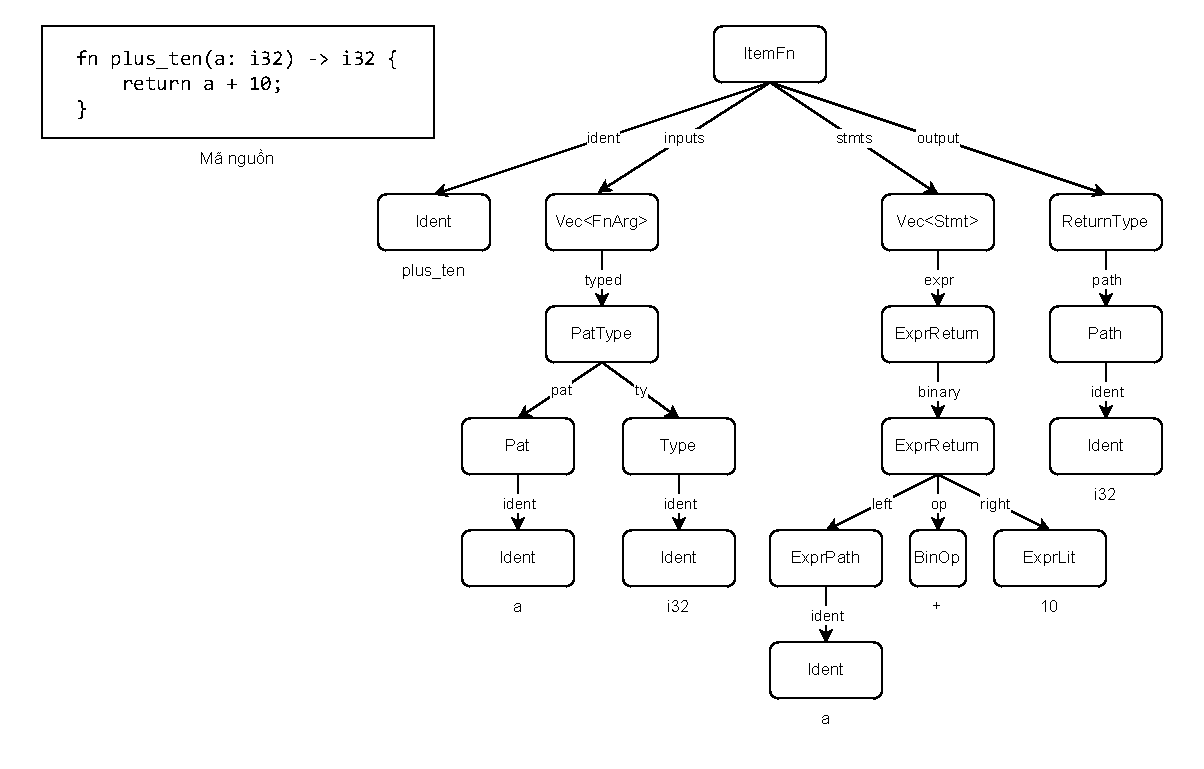
\includegraphics[width=1\columnwidth]{figures/c2/c2_ast.drawio.pdf}
  \centering
  \caption{Ví dụ về cây AST cho mã nguồn Rust.}
  \label{img:c2_ast}
\end{figure}

\subsection{Đồ thị luồng điều khiển}

Đồ thị luồng điều khiển (Control Flow Graph) \cite{yan2019classifying} là đồ thị có hướng, mô tả thứ tự thực thi của các mệnh đề và điều kiện để một mệnh đề được thực thi.
Các nút là các mệnh đề hoặc mệnh đề điều kiện, được nối với nhau bằng các cạnh có hướng, thể hiện thứ tự điều khiển giữa các nút.
Một nút là mệnh đề thì có 1 cạnh ra.
Nếu một nút là mệnh đề điều kiện thì sẽ có 2 cạnh ra, bao gồm một cạnh điều khiển khi điều kiện đúng và một cạnh điều khiển khi điều kiện sai.
CFG được sử dụng cho nhiều ứng dụng phân tích ngữ cảnh, phân tích mã độc hại \cite{gascon2013structural}, định hướng cho công cụ kiểm thử mờ \cite{sparks2007automated}.
Tuy nhiên, CFG không chứa thông tin về luồng dữ liệu, do vậy không đủ toàn diện để ứng dụng phát hiện lỗ hổng bảo mật trong mã nguồn.

\begin{figure}[H]
  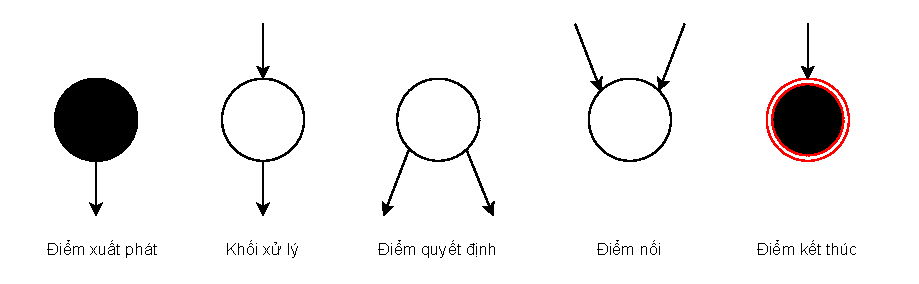
\includegraphics[width=1\columnwidth]{figures/c2/c2_cfg_point.drawio.pdf}
  \centering
  \caption{Các thành phần cơ bản trong đồ thị CFG.}
  \label{img:c2_cfg_point}
\end{figure}

Đồ thị luồng điều khiển bao gồm các thành phần chính là điểm xuất phát, khối xử lý, điểm quyết định, điểm nối và điểm kết thúc.
Trong Hình \ref{img:c2_cfg_point}, \textbf{điểm xuất phát} và \textbf{điểm kết thúc} biểu thị điểm bắt đầu và kết thúc của chương trình, lần lượt được thể hiện bằng hình tròn đặc và hình tròn đặc có viền.
\textbf{Khối xử lý} tượng trưng cho các câu lệnh gán, khai báo và khởi tạo, được thể hiện bằng hình tròn rỗng.
\textbf{Điểm quyết định} biểu thị các câu lệnh điều kiện trong các khối lệnh rẽ nhánh, được thể hiện bằng hình tròn rỗng với hai cạnh đi ra.
\textbf{Điểm nối} biểu thị các câu lệnh thực hiện ngay sau các lệnh rẽ nhánh, có hai cạnh nối đến, được thể hiện bằng hình tròn rỗng.

\begin{figure}[H]
  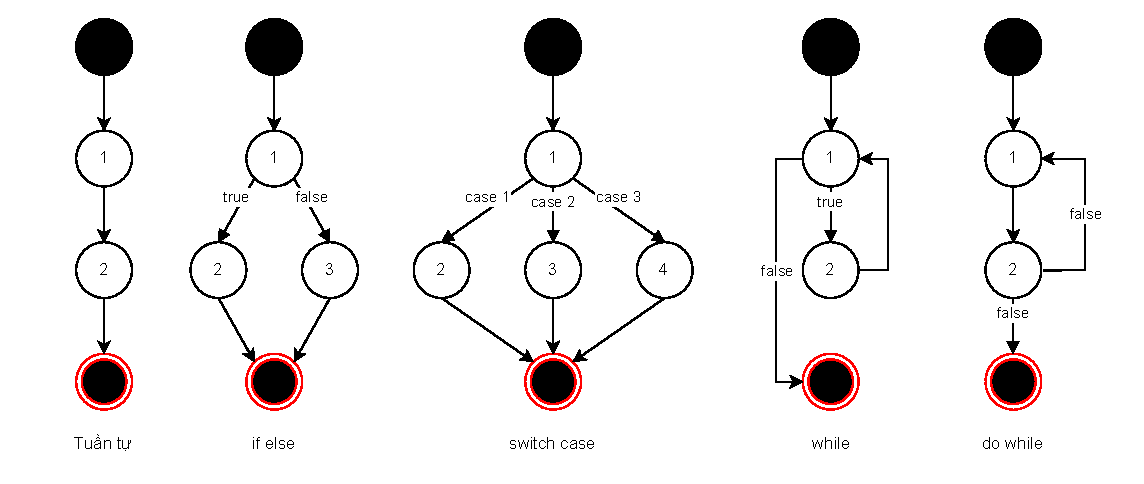
\includegraphics[width=1\columnwidth] {figures/c2/c2_cfg_line.drawio.pdf}
  \centering
  \caption{Các cấu trúc điều khiển phổ biến trong ngôn ngữ lập trình.}
  \label{img:c2_cfg_line}
\end{figure}

Hình \ref{img:c2_cfg_line} mô tả các cấu trúc điều khiển phổ biến có trong các ngôn ngữ lập trình được biểu diễn dưới dạng đồ thị CFG, bao gồm có cấu trúc điều khiển tuần tự, if else, switch case, while và do while.

\subsection{Đồ thị phụ thuộc chương trình}

% The PDG makes explicit both the data and control dependences for each operation in a program. Data dependence graphs have provided some optimizing compilers with an explicit representation of the definition-use relationships implicitly present in a source program [31, 361]. A control flow graph [1, 31] has been the usual representation for the control flow relationships of a program; the control conditions on which an operation depends can be derived from such a graph. An undesirable property of a control flow graph, however, is a fixed sequencing of operations that need not hold. The program dependence graph explicitly represents both the essential data relationships, as present in the data dependence graph, and the essential control relationships, without the unnecessary sequencing present in the control flow graph.’ These dependence relationships determine the necessary sequencing between operations, exposing potential parallelism.

% The PDG represents a program as a graph in which the nodes are statements and predicate expressions (or operators and operands) and the edges incident to a node represent both the data values on which the node’s operations depend and the control conditions on which the execution of the operations depends

Đồ thị phụ thuộc chương trình (Program Dependence Graph) \cite{ferrante1987program} là đồ thị có hướng thể hiện hai khía cạnh của chương trình, phụ thuộc điều khiển và phụ thuộc dữ liệu.
Một nút đại diện cho các mệnh đề hoặc mệnh đề điều kiện, một cạnh thể hiện mối quan hệ phụ thuộc điều khiển hoặc phụ thuộc dữ liệu giữa các nút.
Mệnh đề mà một nút đại diện có được thực thi hay không phụ thuộc vào các cạnh điều kiện điều khiển trỏ tới nút, giá trị của các biến mà mệnh đề sử dụng phụ thuộc vào các cạnh phụ thuộc dữ liệu trỏ tới nút đó.
Lưu ý rằng cạnh phụ thuộc điều khiển không giống như cạnh luồng điều khiển của đồ thị CFG.
Cạnh phụ thuộc điều khiển chỉ thể hiện điều kiện để mệnh đề của một nút được thực thi, không thể hiện thứ tự thực thi của mệnh đề giữa các nút.

\begin{figure}[H]
  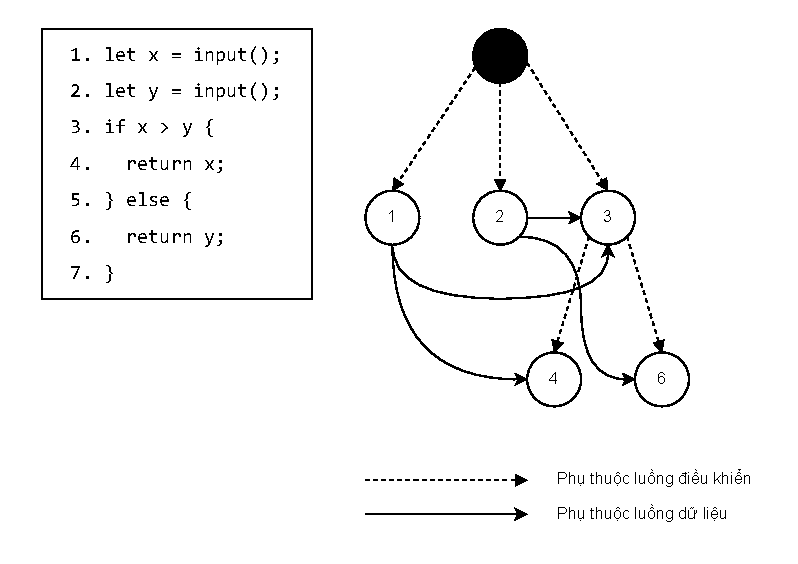
\includegraphics[width=1\columnwidth]{figures/c2/c2_pdg_3.drawio.pdf}
  \centering
  \caption{Ví dụ về đồ thị PDG.}
  \label{img:c2_pdg}
\end{figure}

Hình \ref{img:c2_pdg} biểu diễn ví dụ về một đồ thị PDG với cấu trúc điều kiện if else trong ngôn ngữ Rust, các cạnh nét đứt biểu diễn phụ thuộc điều khiển và các cạnh nét liền biểu diễn phụ thuộc dữ liệu.

\subsection{Đồ thị thuộc tính mã nguồn}

Đồ thị thuộc tính mã nguồn (Code Property Graph) \cite{yamaguchi2014modeling} là một dạng đồ thị biểu diễn mã nguồn hợp thành từ cây AST, đồ thị CFG và đồ thị PDG.
Đồ thị chứa các thông tin về cấu trúc cú pháp, luồng điều khiển và phụ thuộc dữ liệu trong chương trình
Đồ thị CPG tạo ra một lớp biểu diễn trung gian cho mã nguồn mà không bị phụ thuộc vào ngôn ngữ lập trình cụ thể.
Các nút đại diện cho các thành phần như hàm, biến, lớp và các cạnh đại diện cho mối quan hệ giữa chúng như lời gọi hàm, sự gán giá trị, quan hệ cha con hay tham chiếu.
Mỗi nút, cạnh đều có các thuộc tính, mỗi thuộc tính có giá trị riêng.
Đồ thị CPG được ứng dụng để tìm kiếm lỗ hổng trong mã nguồn, phát hiện sao chép mã nguồn bằng học máy, học tăng cường \cite{zhou2019devign, han2023bjxnet}.
Hình \ref{img:c2_cpg_yamaguchi} minh họa một đồ thị CPG cho mã nguồn C \cite{yamaguchi2014modeling}.

% \begin{figure}[H]
%   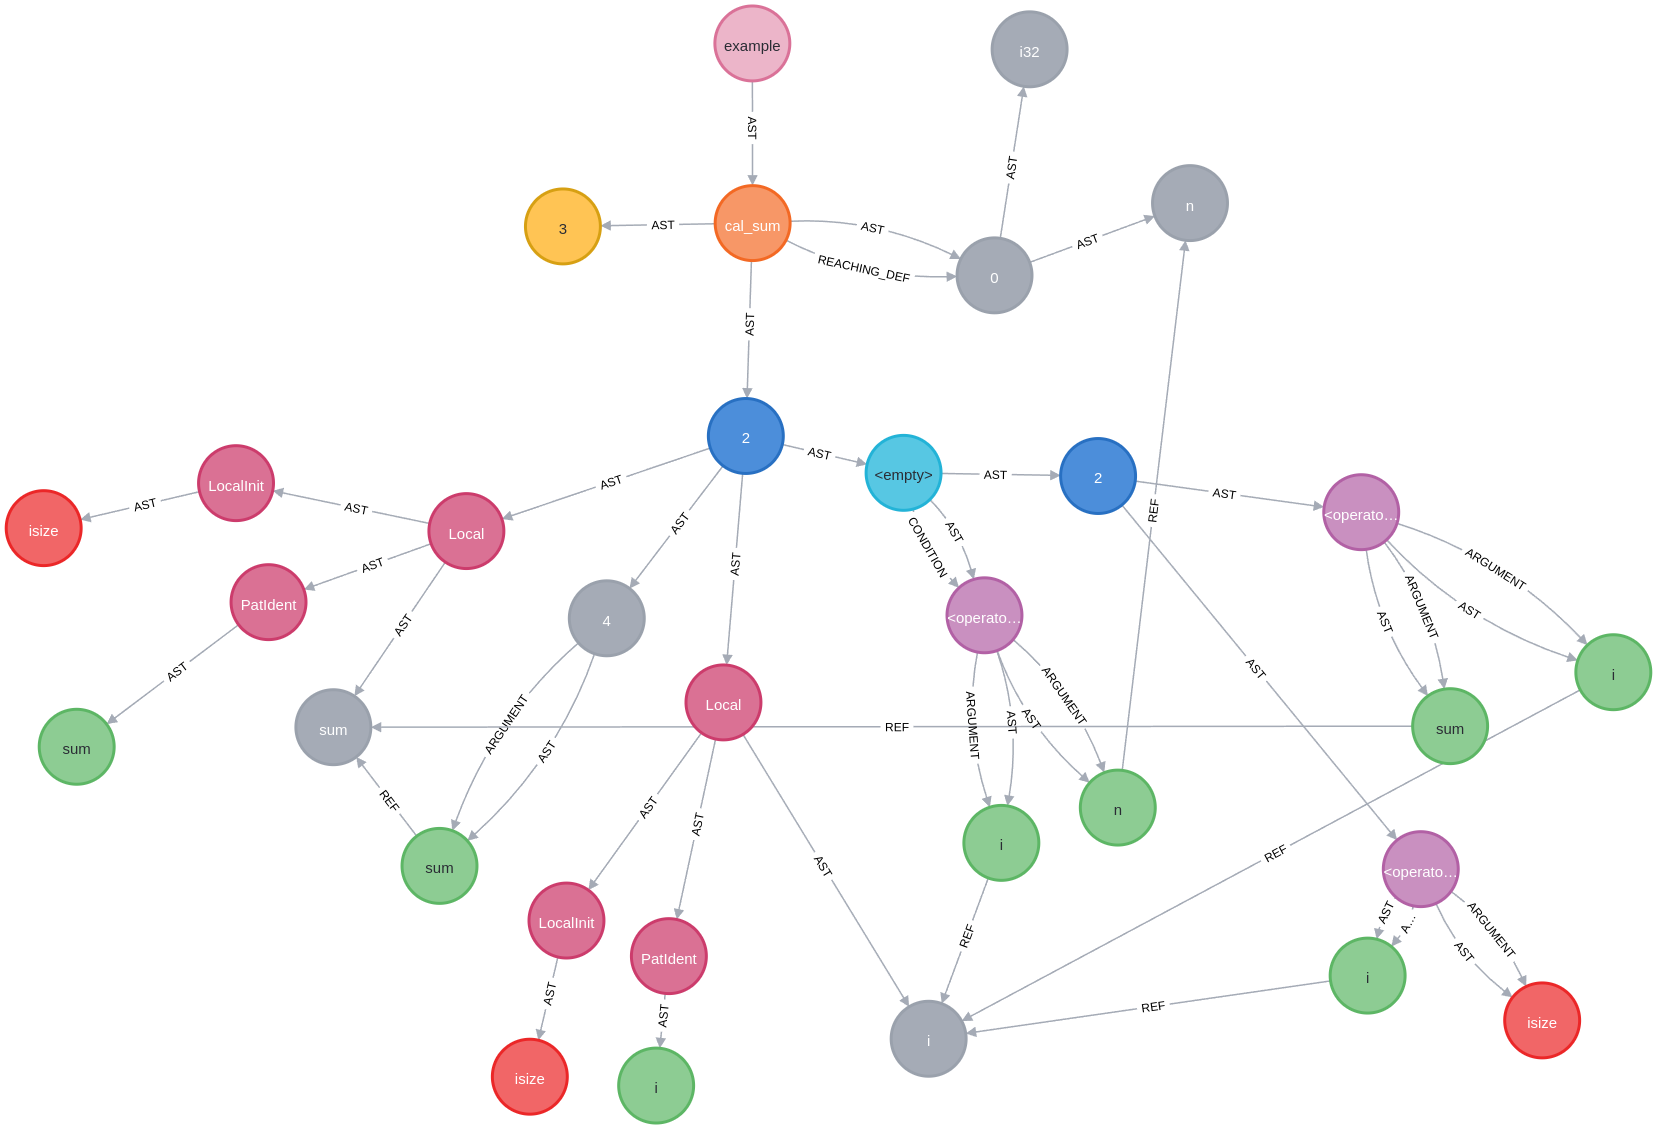
\includegraphics[width=1\columnwidth]{figures/c2/c2_cpg.png}
%   \centering
%   \caption{Minh họa đồ thị CPG.}
%   \label{img:c2_cpg}
% \end{figure}

\begin{figure}[H]
  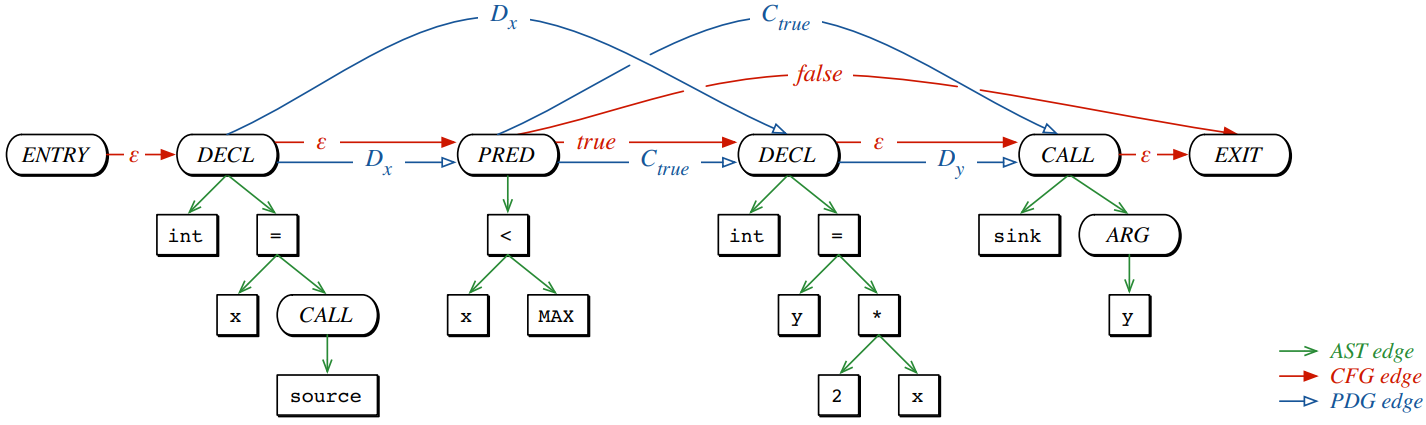
\includegraphics[width=1\columnwidth]{figures/c2/c2_cpg_yamaguchi.png}
  \centering
  \caption{Minh họa đồ thị CPG \cite{yamaguchi2014modeling}.}
  \label{img:c2_cpg_yamaguchi}
\end{figure}


% \begin{listing}[H]
% \begin{minted}[mathescape, breaklines, frame=lines, framesep=2mm, baselinestretch=1.2, fontsize=\footnotesize, linenos]{rust}
% fn cal_sum(n: i32) {
%   let mut sum = 0;
%   let mut i = 1;
%   while i <= n {
%       sum += i;
%       i += 1;
%   }
%   return sum;
% }
% \end{minted}
% \caption{Mã nguồn đầy đủ cho đồ thị CPG Hình \ref{img:c2_cpg}.}
% \label{code:c2_cpg}
% \end{listing}

\section{Công cụ Joern}

\subsection{Đặc tả đồ thị thuộc tính mã nguồn của Joern}

Đồ thị thuộc tính mã nguồn đã được nghiên cứu rộng rãi, có rất nhiều phiên bản cài đặt được xây dựng dành cho các mục đích khác nhau \cite{yamaguchi2014modeling, xiaomeng2018cpgva, kuchler2022representing, githubGitHubWimkeirgraft, githubGitHubPlumeossplume, joernJoernHunteraposs, fraunhoferaisecHomeCode, banse2021cloud, weiss2022language, keirsgieter2020graft}.
Tuy nhiên có một phiên bản mã nguồn mở được do chính tác giả của đồ thị thuộc tính mã nguồn, Fabian Yamaguchi, đích thân phát triển và duy trì có tên Joern \cite{joernJoernHunteraposs}.

Dự án CPG [6, 8] cho phép biểu diễn mã nguồn của các ngôn ngữ lập trình khác nhau dưới dạng đồ thị.
Cho đến nay, trọng tâm là Java và C/C++ nhưng hỗ trợ thử nghiệm cho Python, Go và TypeScript cũng có sẵn.
Mục tiêu của dự án là cung cấp một cách biểu diễn mã nguồn không phụ thuộc vào ngôn ngữ.
Điều này cho phép chuyên gia bảo mật xác định các lỗ hổng hoặc lỗi.
Hơn nữa, thư viện CPG bao gồm một cách để lưu trữ đồ thị trong neo4j2 và làm cho đồ thị có thể truy cập qua giao diện dòng lệnh.
Trong một số trường hợp, thư viện cũng có thể đánh giá giá trị mà một nút có thể giữ.
Tất cả những điều này cho phép chuyên gia bảo mật viết các truy vấn tùy chỉnh cho cơ sở dữ liệu đồ thị hoặc cách biểu diễn CPG trong bộ nhớ.
Thư viện CPG được thiết kế để cho phép tái sử dụng các truy vấn này giữa tất cả các ngôn ngữ lập trình được hỗ trợ.
Để đạt được mục tiêu này, thư viện CPG thực hiện một hệ thống phân cấp lớp đầy đủ, bao gồm các loại câu lệnh và biểu thức khác nhau.
CPG mã hóa thông tin như hệ thống phân cấp lớp của mã đang được phân tích, đồ thị luồng điều khiển và đồ thị cuộc gọi trong một đồ thị duy nhất.
Thiết kế hiện tại chủ yếu nhắm vào các ngôn ngữ lập trình hướng đối tượng.
Để đối phó với khả năng thiếu một số đoạn mã hoặc lỗi trong mã, thư viện có khả năng chịu lỗi với mã không đầy đủ, không biên dịch được và thậm chí ở mức độ nào đó còn không chính xác.

% Đồ thị thuộc tính mã nguồn (Code Property Graph - CPG) là một cấu trúc dữ liệu được thiết kế để khai thác các cơ sở mã nguồn lớn nhằm tìm kiếm các mẫu lập trình.
% Những mẫu này được hình thành trong một ngôn ngữ đặc thù (DSL) dựa trên Scala.
% CPG đóng vai trò như một biểu diễn chương trình trung gian duy nhất cho tất cả các ngôn ngữ được Joern và phiên bản thương mại của nó là Ocular hỗ trợ.

% Đồ thị thuộc tính là một trừu tượng chung được hỗ trợ bởi nhiều cơ sở dữ liệu đồ thị đương đại như Neo4j, OrientDB và JanusGraph.
% Trên thực tế, các phiên bản cũ của Joern đã sử dụng các cơ sở dữ liệu đồ thị mục đích chung làm nơi lưu trữ và ngôn ngữ truy vấn đồ thị Gremlin.
% Tuy nhiên, khi những hạn chế của cách tiếp cận này trở nên rõ ràng theo thời gian, chúng tôi đã thay thế cả hệ thống lưu trữ và ngôn ngữ truy vấn bằng cơ sở dữ liệu đồ thị OverflowDB của riêng mình.

Các thành phần cấu thành đồ thị thuộc tính mã nguồn bao gồm:

\begin{itemize}
  \item \textbf{Các nút và loại của chúng:} Các nút đại diện cho các thành phần của chương trình.
  Điều này bao gồm các cấu trúc ngôn ngữ cấp thấp như phương thức, biến, và cấu trúc điều khiển, cũng như các cấu trúc cấp cao hơn như điểm cuối HTTP hoặc các kết quả phân tích.
  Mỗi nút có một loại, loại này chỉ ra loại thành phần chương trình mà nút đó đại diện, ví dụ, một nút với loại METHOD đại diện cho một phương thức, trong khi một nút với loại LOCAL đại diện cho khai báo của một biến cục bộ.
  \item \textbf{Cạnh có nhãn:} Quan hệ giữa các thành phần chương trình được biểu diễn thông qua các cạnh giữa các nút tương ứng của chúng.
  Ví dụ, để biểu thị rằng một phương thức chứa một biến cục bộ, chúng ta có thể tạo một cạnh với nhãn CONTAINS từ nút của phương thức đến nút của biến cục bộ.
  Bằng cách sử dụng các cạnh có nhãn, chúng ta có thể biểu diễn nhiều loại quan hệ khác nhau trong cùng một đồ thị.
  Hơn nữa, các cạnh có hướng để biểu thị, ví dụ, rằng phương thức chứa biến cục bộ nhưng không phải ngược lại.
  Nhiều cạnh có thể tồn tại giữa cùng hai nút.
  \item \textbf{Cặp khóa-giá trị:} Các nút mang các cặp khóa-giá trị (thuộc tính), trong đó các khóa hợp lệ phụ thuộc vào loại nút.
  Ví dụ, một phương thức có ít nhất tên và chữ ký, trong khi một khai báo biến cục bộ có ít nhất tên và loại của biến được khai báo.
\end{itemize}

Tóm lại, đồ thị thuộc tính mã nguồn là các đồ thị có hướng, được gán nhãn cạnh, và chứa các thuộc tính, và chúng tôi khẳng định rằng mỗi nút mang ít nhất một thuộc tính chỉ ra loại của nó.
Điều này giúp cho việc phân tích mã nguồn trở nên dễ dàng và hiệu quả hơn, đồng thời mở ra nhiều khả năng cho việc tìm kiếm và phát hiện các mẫu lập trình trong các cơ sở mã nguồn lớn.

\begin{itemize}
  \item Đặc tả CPG của Joern được thiết kết chủ yếu cho ngôn ngữ C/C++ và Java, đưa ra các chuẩn chung như (if else, swtich case, while, for, ...) mà nhiều ngôn ngữ khác có điểm tương đồng như Python, Go, TypeScript, ... có thể tuân thủ.
  \item Tuy nhiên chuẩn chung này không thể đáp ứng được nhu cầu của tất cả các ngôn ngữ. Joern tập trung cho 2 ngôn ngữ lớn là C/C++ và Java do vậy sẽ đặc tả có sẵn (hiện có) sẽ phù hợp với các ngôn ngữ có cú pháp C-like và hướng đối tượng (OOP)
  \item Trong khi đó Rust là một ngôn ngữ lập trình mới, có cú pháp dựa trên C-Like nhưng vẫn có đôi chút sự khác biệt vì đây là ngôn ngữ hiện đại, hỗ trợ đan xen cả hướng đối tượng và hướng hàm. Đặc biệt với tính hướng hàm, Rust có nhiều cú pháp mới mà Joern chưa hỗ trợ, hay những biểu thức, mệnh đề trong C/C++ hay Java là không hợp lệ nhưng trong Rust thì hoàn toàn có thể
  \item Nhìn chung bản đặc tả CPG của Joern cung cấp 1 baseline bao phủ các tính năng phổ biến mà ngôn ngữ lập trình nào cũng có (cùng ý nghĩa nhưng có thể sử dụng cú pháp, keyword khác nhau) như $if\ else$, ... nhưng không thể đáp ứng được tất cả các ngôn ngữ lập trình hiện đại. Do vậy đối với từng ngôn ngữ riêng biệt vẫn phải bổ sung thêm các đặc tả mới cho phù hợp với từng ngôn ngữ, đặc biệt là Rust có cơ chế quản lý bộ nhớ an toàn thể hiện qua các tính năng $ownership$, $borrowing$, $lifetime$ mà Joern chưa hỗ trợ, và cả tính năng hướng hàm
\end{itemize}

\textbf{Joern Backend, Joern Frontend}

\begin{figure}[H]
  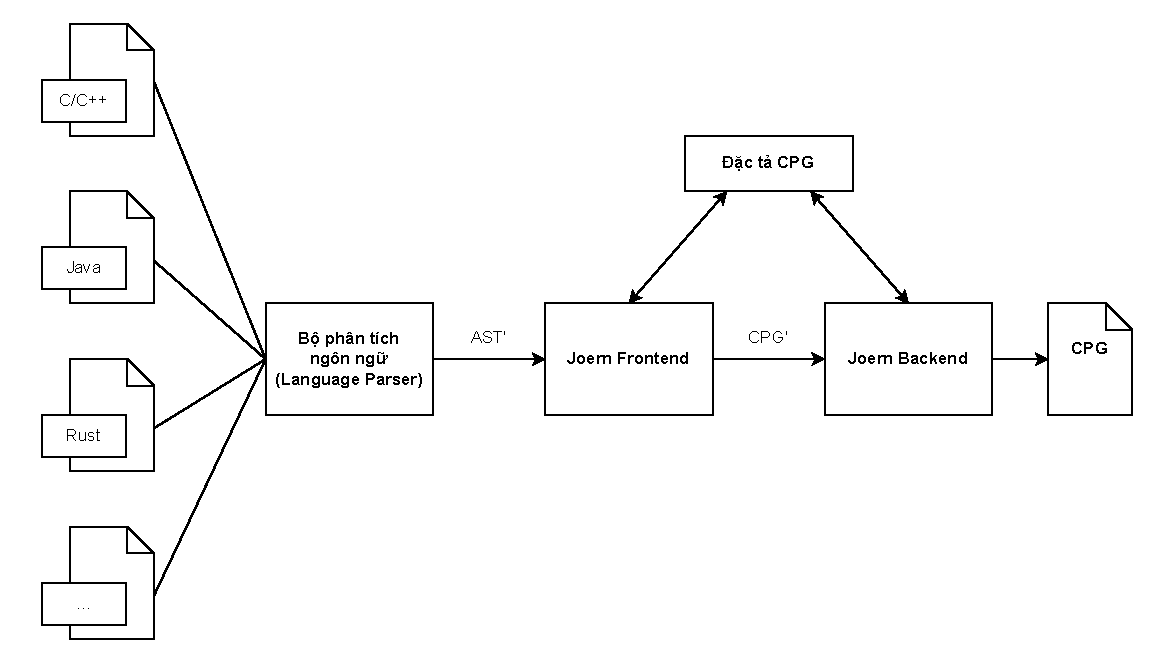
\includegraphics[width=1\columnwidth]{figures/c2/c2_frontend_backend.drawio.pdf}
  \centering
  \caption{Cách hoạt động của công cụ Joern.}
  \label{img:c2_frontend_backend}
\end{figure}

\begin{itemize}
  \item Ngoài phần đặc tả CPG dùng chung cho nhiều ngôn ngữ trên lý thuyết, Joern còn cung cấp 1 kiến trúc cài đặt thực tế có tính mở rộng cao, tương ứng với đặc tả CPG. Joern hiển tại hỗ trợ rất nhiều ngôn ngữ C/C++, Java, Python, Go, TypeScript, ... Để có thể hỗ trợ được nhiều ngôn ngữ như vậy thì Joern sử dụng 2 thành phần chính là Joern Frontend và Joern Backend, đây là 2 thành phần có tính tái sử dụng cao, không phụ thuộc vào ngôn ngữ
  \item Luồng hoạt động của kiến trúc Joern như sau. Mỗi ngôn ngữ có tập các cú pháp khác nhau, tương ứng cũng sẽ có định nghĩa về cây AST khác nhau, đây là phần người dùng muốn mở rộng Joern cho 1 ngôn ngữ mới cần phải tự đảm nhiệm. Mã nguồn của 1 ngôn ngữ sau được được công cụ Language Parser chuyển thành cây $AST*$. Cây $AST*$ ở đây không nhất thiết chỉ dừng ở đúng mức độ thông tin là 1 cây AST mà có thể bổ sung thêm thông tin khác như kiểu dữ liệu, vị trí trong mã nguồn, ... nhưng tối thiểu đảm bảo đủ thông tin là 1 cây AST tối thiểu. Ví dụ như các ngôn ngữ có sự phát triển lâu dài như C/C++ hay Java sử dụng CDT/ JDT để làm Language Parser. CDT/JDT là công cụ rất mạnh, được dùng trong các IDE nên số lượng thông tin rất đáng kể. Còn những ngôn ngữ hiện đại như Rust, Go thì các công cụ như này chưa được phát triển toàn diện nên thông tin của cây $AST*$ chưa được đầy đủ. \item Sau khi có cây $AST*$, cây này sẽ được biến đổi thành đồ thị thuộc tính mã nguồn (CPG) theo định nghĩa đặc tả CPG. Đây là công việc của Joern Frontend. Joern Frontend sẽ đọc cây $AST*$ và chuyển đổi thành đồ thị thuộc tính mã nguồn (CPG) theo đặc tả CPG. Joern Frontend đối với từng ngôn ngữ cũng là công việc cần thực hiện, do công việc thực tế cần làm là chuyển đổi cấu trúc dữ liệu của cây $AST*$ sang cấu trúc dữ liệu tương ứng của định nghĩa $CPG$. Joern Frontend đóng vai trò chuyển đổi cây $AST*$ sang cây $CPG$, $CPG$ bổ sung thông tin thành đồ thị $CPG$
  \item Sau khi được Joern Frontend xử lý, ta sẽ có được đồ thị $CPG*$ nhưng đồ thị $CPG*$ này là đồ thị không hoàn chỉnh. Để hoàn thiện được đồ thị $CPG$ thì ta cần phải sử dụng đến Joern Backend. Ở bước Joern Frontend, ta thực hiện bước chuyển đổi 1 node AST thành 1 node CPG, tạo thêm các cạnh để thể hiện các mối quan hệ giữa các node, tuy nhiên các cạnh này chưa thể hiện được đầy đủ đồ thị CPG bao gồm AST, CFG, PDG. Với cấu trúc dữ liệu CPG của Joern, ta chỉ cần định nghĩa 1 phần số cạnh, node cần thiết của đồ thị CPG, phần còn lại sẽ được Joern Backend thực hiện các thuật toán logic để có thể tự động suy diễn các mối quan hệ còn lại. Ví dụ trong cây AST có nút thể hiện vòng lặp $for$, ta chuyển thành nút $for$ của CPG kèm thêm 1 số thông tin như mệnh đề điều kiện, biến chỉ số vòng lặp (index). Joern Backend nắm được thông tin này thì có thể tự động suy diễn ra các mối quan hệ như $REACHING_DEF$ (du pair), $DOMINATOR$, $POST\ DOMINATOR$, $CONTROL\ DEPENDENCY$, $DATA\ DEPENDENCY$, $CONTROL\ FLOW$, $DATA\ FLOW$, ... từ đó tạo ra đồ thị CPG hoàn chỉnh. Chú ý CPG được cấu tạo từ 3 thành phần AST, CPG, PDG. Trong Joern thông tin của 3 thành phần này được chia thành 3 lớp, 1 đồ thị CPG được cấu tạo từ nhiều lớp trồng lên nhau, có thể sinh ra CPG chỉ có lớp AST, hoặc AST + CPG, hoặc AST + CPG + PDG. Hoàn toàn có thể mở rộng viết thêm các lớp khác nếu cần thiết, ví dụ như bổ sung 1 lớp thông tin về bảo mật, an toàn bộ nhớ, hay cụ thể trong Rust là lớp chứa thông tin $ownership$, $borrowing$, $lifetime$
  \item Sau khi toàn bộ thông tin của CPG được hoàn chỉnh dựa trên các lớp, dữ liệu CPG được xuất ra thành file binary, cấu trúc dữ liệu đồ thị. Dữ liệu này có thể được sử dụng để truy vấn thông qua các engine cơ sở dữ liệu đồ thị như neo4j, OrientDB, JanusGraph, ... hoặc có thể được sử dụng để phân tích, tìm kiếm thông qua các công cụ khác như Joern CLI, Joern Scan, Joern Slice, Joern Flow, Joern Export, Joern Vectors
\end{itemize}

\subsection{Bộ công cụ của Joern}

\begin{figure}[H]
  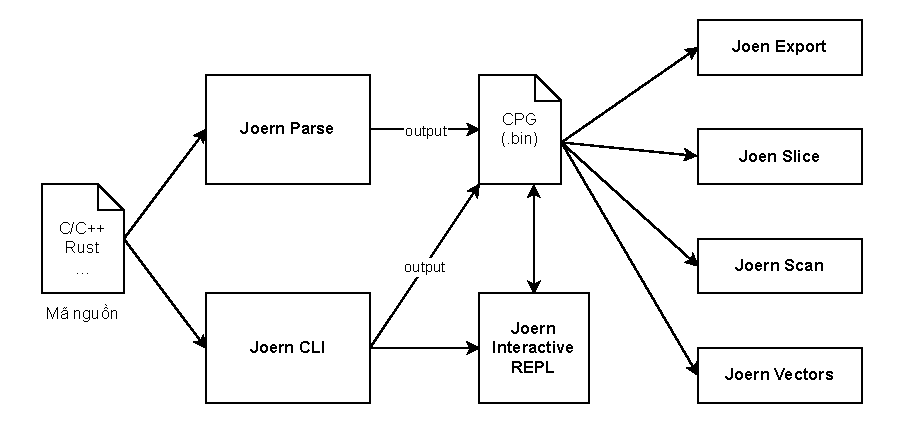
\includegraphics[width=1\columnwidth]{figures/c2/c2_joern_tools.drawio.pdf}
  \centering
  \caption{Các công cụ xung quanh Joern.}
  \label{img:c2_joern_tools}
\end{figure}

\begin{itemize}
  \item Không chỉ cung cấp kiến trúc để có thể biến đổi mã nguồn từ một ngôn ngữ sang đồ thị thuộc tính mã nguồn. Joern cần cung cấp 1 loạt các cung cấp để khai thác thông tin từ đồ thị thuộc tính mã nguồn sinh ra. Các công cụ này bao gồm: Joern Scan, Joern Slice, Joern Flow, Joern Export, Joern Vectors
  \item \textbf{JoernExport}: https://docs.joern.io/export/
  Dump intermediate graph representations (or entire graph) of code in a given export format
  Joern is used in academic research as a source for intermediate graph representations of code, particularly in machine learning and vulnerability discovery applications [e.g., 1,2,3,4,5]. To support this use-case, Joern provides both plotting capabilities in the interactive console as well as the joern-export command line utility.
  You can also export the entire graph into a neo4j csv format (along with instructions on how to import it into a running neo4j instance), graphml, graphson or graphviz dot:
  \item \textbf{JoernParse}: parse ra output ngay lập tức hoặc lưu vào cơ sở dữ liệu, không traverl
  \item \textbf{JoernSlice}: Extract various slices from the CPG.
  https://docs.joern.io/cpg-slicing/
  joern-slice is the entrypoint for Joern’s CPG slicing mechanism and specifies ways to extract useful subsets of information from the CPG. Two modes are available:
  Data-flow: This is a pretty standard backwards data-flow slicing command that starts at call arguments and slices backwards to create a graph of slices.
  Usages: This targets locals and parameters and traces what calls they make and in which calls they are used. This is useful for describing how a variable interacts in a procedure.
  \item \textbf{JoernScan}: Creates a code property graph and scans it with queries from installed bundles. QueryDB
  https://docs.joern.io/scan/
  Joern Scan ships with a default set of queries, the Joern Query Database. This set of queries is constantly updated, and contributions are highly encouraged https://github.com/joernio/joern/tree/master/querydb.
  \item \textbf{JoernVectors}: Extract vector representations of code from CPG, JoernFlow: Find flows, JoernCLI: REPL for Joern
\end{itemize}

Joern là một nền tảng mạnh mẽ dành cho việc phân tích mã nguồn, bytecode và mã nhị phân.
Công cụ này tạo ra các đồ thị thuộc tính mã nguồn (code property graphs), một cách biểu diễn đồ thị của mã giúp cho việc phân tích mã nguồn đa ngôn ngữ trở nên dễ dàng hơn.
Các đồ thị thuộc tính mã nguồn được lưu trữ trong một cơ sở dữ liệu đồ thị tùy chỉnh, cho phép khai thác mã nguồn thông qua các truy vấn tìm kiếm được xây dựng trong một ngôn ngữ truy vấn đặc thù dựa trên Scala.
Joern được phát triển với mục tiêu cung cấp một công cụ hữu ích cho việc khám phá lỗ hổng bảo mật và nghiên cứu phân tích chương trình tĩnh.

Joern hỗ trợ các nhà phát triển và nhà nghiên cứu trong việc tìm kiếm và xác định các điểm yếu tiềm ẩn trong mã nguồn, giúp nâng cao chất lượng và bảo mật của phần mềm.
Bên cạnh đó, Joern còn có khả năng phân tích mã nguồn đa ngôn ngữ, giúp các nhóm phát triển có thể làm việc với nhiều ngôn ngữ lập trình khác nhau mà không gặp trở ngại về công cụ.
Với khả năng truy vấn mạnh mẽ và linh hoạt, Joern đã trở thành một công cụ quan trọng trong việc phân tích mã nguồn và phát hiện các lỗ hổng bảo mật.
Bạn có thể tìm hiểu thêm về Joern tại địa chỉ https://joern.io/.

Joern hỗ trợ nhiều ngôn ngữ lập trình khác nhau.
Các ngôn ngữ được hỗ trợ bao gồm C/C++, Java, JavaScript, Python, x86/x64, JVM Bytecode, Kotlin, PHP, Rust, Swift, Ruby và C\#.
Điều này cho thấy Joern có khả năng phân tích mã nguồn đa ngôn ngữ, giúp các nhà phát triển và nhà nghiên cứu có thể làm việc với nhiều ngôn ngữ lập trình khác nhau mà không gặp trở ngại về công cụ.
Tuy nhiên, Joern chưa hỗ trợ cho ngôn ngữ Rust.

\newpage\cleardoublepage
% \chapter{Luồng hoạt động và kiến trúc công cụ}
\chapter{Thiết kế và cài đặt công cụ}
\label{chap:method}

Chương 3 trình bày về quy trình phân tích mã nguồn cho ngôn ngữ Rust bao gồm việc xây dựng cây AST và ánh xạ từ cây AST sang đồ thị CPG.
Chương cũng sẽ đi sâu vào kiến trúc, các thành phần và cài đặt của công cụ.
% Tiếp theo, các thể loại cú pháp Rust ...
% Ngoài ra, chương cũng sẽ trình bày về các hạn chế hiện thời của công cụ.
Tiếp theo, các thể loại cú pháp Rust sẽ được phân tích để minh họa cách ánh xạ từ cây AST sang đồ thị CPG một cách hiệu quả.
Ngoài ra, chương cũng sẽ trình bày về các hạn chế hiện thời, nhằm làm rõ các thách thức và định hướng cải tiến công cụ trong tương lai.

% Nội dung của chương 4 là về việc chuy`ển đổi mã nguồn sang đồ thị CPG trên các thể loại cú pháp Rust.
% Mức độ cài đặt của công cụ cho việc bao phủ các loại nút AST và ánh xạ chúng sang nút CPG tương ứng sẽ được thảo luận.
% Ngoài ra, chương cũng sẽ trình bày về các hạn chế hiện thời của công cụ.

% \section{Luồng hoạt động}
\section{Luồng hoạt động và cài đặt công cụ}

\begin{figure}[H]
	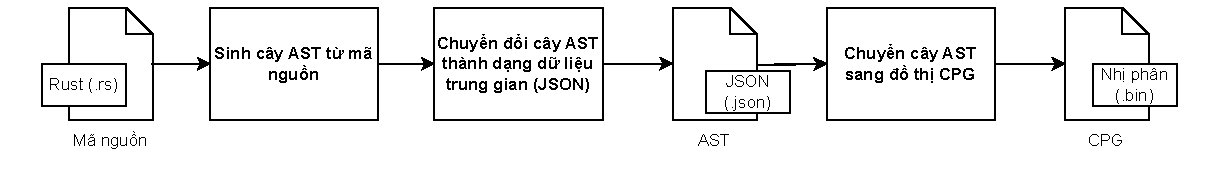
\includegraphics[width=1\columnwidth]{figures/c3/c3_flow_2.drawio.pdf}
	\centering
	\caption{Quy trình phân tích mã nguồn Rust.}
	\label{img:c3_flow_2}
\end{figure}

% \begin{figure}[H]
% 	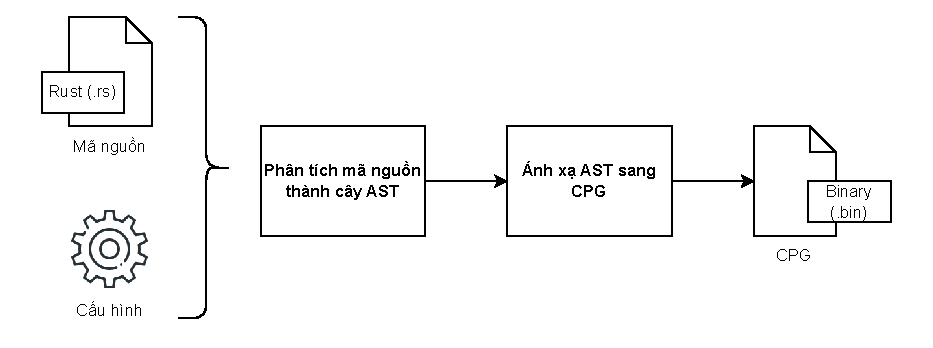
\includegraphics[width=1\columnwidth]{figures/c3/c3_flow.drawio.pdf}
% 	\centering
% 	\caption{Quy trình phân tích mã nguồn Rust.}
% 	\label{img:c3_flow}
% \end{figure}

% \begin{figure}[H]
% 	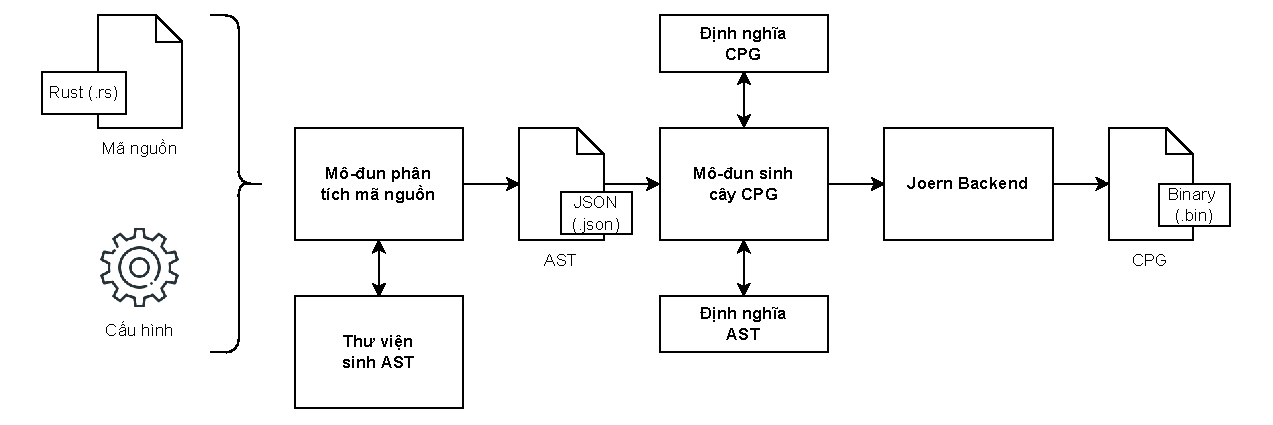
\includegraphics[width=1\columnwidth]{figures/c4/c4_install_flow.drawio.pdf}
% 	\centering
% 	\caption{Kiến trúc công cụ.}
% 	\label{img:c4_install_flow}
% \end{figure}

% \begin{figure}[H]
% 	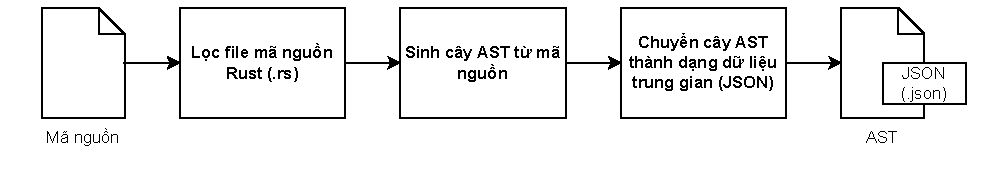
\includegraphics[width=1\columnwidth]{figures/c3/c3_flow_ast.drawio.pdf}
% 	\centering
% 	\caption{Quy trình xây dựng cây AST.}
% 	\label{img:c3_flow_ast}
% \end{figure}

Mục tiêu của công cụ là phân tích mã nguồn Rust và xây dựng đồ thị CPG biểu diễn mã nguồn đó.
% Đầu vào của công cụ là các tệp mã nguồn Rust, đầu ra là đồ thị CPG lưu dưới dạng nhị phân.
Đầu vào của công cụ là các tệp mã nguồn Rust, trong khi đầu ra là đồ thị CPG được lưu dưới dạng nhị phân để dễ dàng xử lý và lưu trữ.
Đồ thị CPG được phục vụ cho việc thực hiện các câu lệnh truy vấn trên đồ thị hoặc quét đồ thị để tìm lỗ hổng trong mã nguồn.
% Với yêu cầu đầu vào, đầu ra như trên, luồng hoạt động của công cụ bao gồm các bước được thể hiện trong hình \ref{img:c3_flow_2}.
Với yêu cầu đầu vào và đầu ra như trên, luồng hoạt động của công cụ được thiết kế thành các bước liên kết chặt chẽ và được thể hiện trong hình \ref{img:c3_flow_2}.
% Chi tiết các bước được tiến hành như sau:
% Các bước này bao gồm phân tích cú pháp mã nguồn, xây dựng cây AST, ánh xạ cây AST sang đồ thị CPG, và cuối cùng là xuất đồ thị dưới định dạng nhị phân.
Chi tiết các bước được tiến hành như sau:

\begin{enumerate}
	\item Từ thư mục của dự án, lọc lấy các tệp mã nguồn Rust (các tệp có đuôi \texttt{.rs}).
	\item Với mỗi tệp mã nguồn, sử dụng thư viện \textit{syn} \cite{synRust} để sinh cây AST từ nội dung mã nguồn của tệp đó.
	\textit{syn} là một thư viện phân tích mã nguồn thành cây AST được sử dụng rộng rãi với nhiều mục đích, trong đó bao gồm việc cài đặt tính năng Procedural Macro \cite{rustlangProceduralMacros} của Rust.
	Tính tới thời điểm hiện tại Rust không có đặc tả ngôn ngữ chính thức, do đó cộng đồng sử dụng Rust Reference \cite{rustReference} coi như phiên bản sát nhất so với một đặc tả ngôn ngữ.
	Thư viện syn xây dựng định nghĩa các nút của cây AST tuân theo Rust Reference.
	\item Chuyển đổi cây AST từ ngôn ngữ Rust sang định dạng JSON.
	Joern có thể được sử dụng cho nhiều ngôn ngữ và Joern Frontend không phụ thuộc vào bộ phân tích ngôn ngữ của một ngôn ngữ nhất định, do vậy cần có định dạng dữ liệu trung gian để chuyển đổi cây AST của bộ phân tích ngôn ngữ sang ngôn ngữ Scala của Joern Frontend.
	Có các kiểu dữ liệu trung gian phổ biến như JSON, XML, YAML, trong đó JSON được lựa chọn bởi tính đơn giản, dễ chuyển đổi.
	\item Cây AST dưới định dạng JSON được đọc ngược lại bằng mã nguồn Scala của Joern Frontend.
	Từ đây ta sẽ thực hiện chuyển đổi cây AST sang đồ thị CPG, từng loại nút trong cây AST sẽ có ánh xạ tương ứng với một loại nút trong đồ thị CPG.
	Các thông tin trong cây AST sẽ được khai thác để xây dựng nút CPG phù hợp, thông tin giữa các nút AST được sử dụng để xây dựng các cạnh, thuộc tính cho cạnh và nút trong đồ thị CPG.
	Quá trình xây dựng đồ thị CPG sẽ bao gồm vai trò của Joern Frontend và Joern Backend, quá trình này sẽ được mô tả chi tiết ở phần \ref{chapter:arch}.
	\item Cuối cùng, đồ thị CPG được lưu dưới dạng tệp nhị phân và đây là đầu ra kì vọng của công cụ.
\end{enumerate}

\textbf{Về cài đặt,} thư viện syn phiên bản \href{https://docs.rs/syn/2.0.87/syn/}{v2.0.87} có định nghĩa của 162 \texttt{struct} tương ứng với 162 loại nút AST và 33 \texttt{enum} tương ứng với 33 loại nút AST đa hình.
Hiện tại công cụ đã ánh xạ 162 loại nút AST và 33 loại nút AST đa hình ở trên thành loại nút CPG tương ứng, tức là \textbf{100\% định nghĩa các loại nút AST đã được ánh xạ sang nút CPG tại phiên bản hiện thời}.
\href{https://github.com/congnghiahieu/rust-parser/blob/master/docs/MAPPING.md}{Địa chỉ bảng tổng hợp ánh xạ các loại nút AST sang loại nút CPG tương ứng.}

Công cụ được thực hiện kiểm thử trên 151 tệp mã nguồn bao gồm đa dạng các thể loại cú pháp, thu thập từ trang \href{https://doc.rust-lang.org/stable/rust-by-example/index.html}{Rust By Example} thuộc Rust Foundation \cite{rustlangRustFoundation}.
Ngoài ra, việc chuyển đổi từ AST sang CPG được kiểm tra trên 20 dự án lớn nằm trong 100 dự án Rust có lượng sao lớn nhất trên Github \cite {githubGithubRankingTop100RustmdMaster}.
Mã nguồn của công cụ được lưu trữ tại địa chỉ \href{https://github.com/congnghiahieu/rust-parser}{rust-parser}, \href{https://github.com/congnghiahieu/syn-serde}{syn-serde}, \href{https://github.com/congnghiahieu/joern}{joern}, \href{https://github.com/congnghiahieu/codepropertygraph}{codepropertygraph}.

\section{Kiến trúc công cụ}

\begin{figure}[H]
	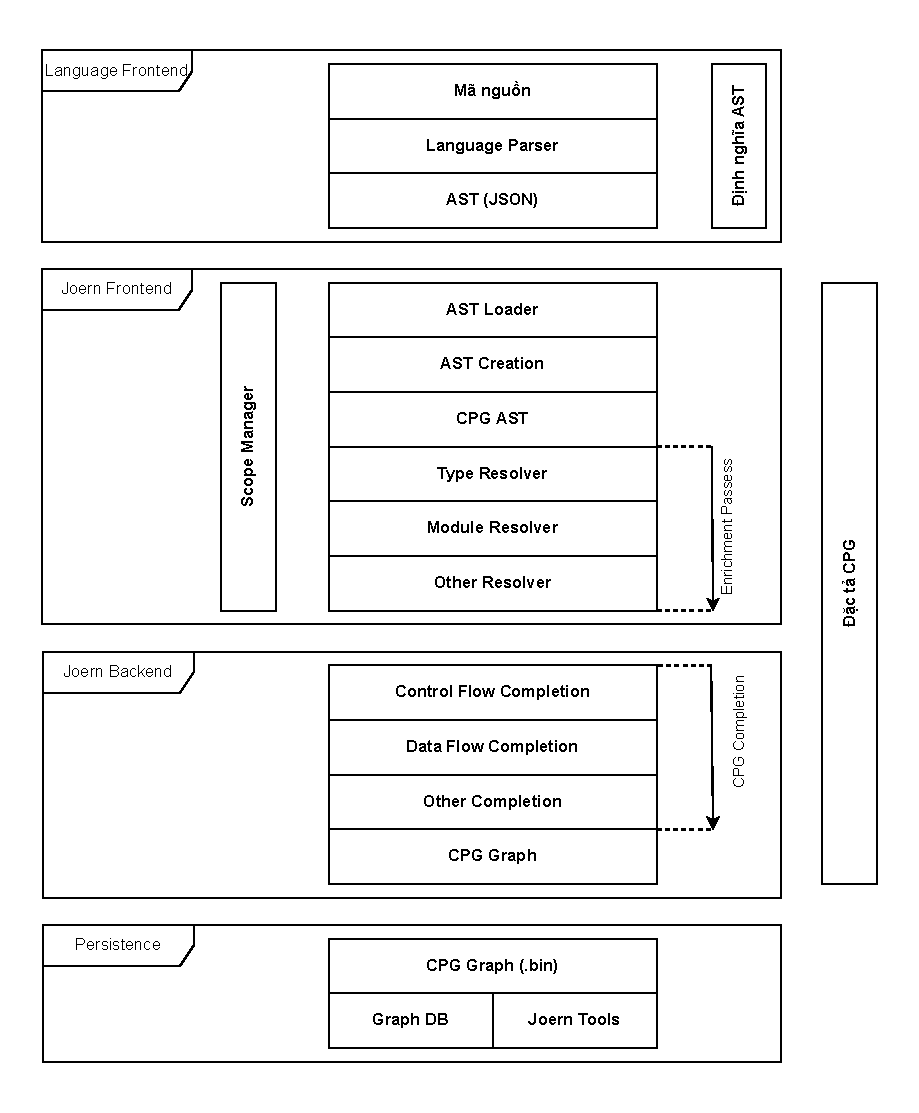
\includegraphics[width=1\columnwidth]{figures/c3/c3_arch.drawio.pdf}
	\centering
	\caption{Kiến trúc công cụ.}
	\label{img:c3_arch}
\end{figure}

Do sử dụng công cụ joern nên kiến trúc của công cơ về cơ bản sẽ là kiến trúc của Joern và mở rộng thêm. Phần này sẽ đi chi tiết hơn so với phần \ref{sec:joern_flow} đã trình bày ở phía trên. Các thành phần chính của công cụ bao gồm:

\textbf{Language Frontend} là phần đặc thù của mỗi ngôn ngữ lập trình, người dùng cần tự đảm nhiệm phần này khi muốn mở rộng công cụ Joern cho ngôn ngữ lập trình mới. Nhiệm vụ của Language Frontend là chuyển đổi mã nguồn thành cây AST dựa trên định nghĩa AST của đặc tả ngôn ngữ. Language Frontend có thể được cài đặt bằng bất cứ ngôn ngữ nào, do đó để có thể chuyển tiếp dư liệu cho quá trình tiếp theo, Language Frontend cần xuất cây AST ra dữ liệu trung gian, ở đây là JSON.

\textbf{Joern Frontend} là nơi chính thực hiện các công việc chuyển đổi cây AST của một ngôn ngữ lập trình cụ thể thành cây CPG theo đặc tả CPG. Đặc tả CPG sẽ được sử dụng xuyên suốt trong cả Joern Frontend và Joern Backend.
Joern Frontend sẽ nhận dữ liệu từ Language Frontend dưới dạng JSON bằng AST Loader. Cây AST sau khi được nạp vào Joern Frontend dưới ngôn ngữ Scala thì sẽ được chuyển đổi thành cây CPG bởi AST Creation. AST Creation thực hiện ánh xạ mỗi một loại nút AST của ngôn ng
sang một loại nút CPG tương ứng. Không chỉ tạo nút, AST Creation còn tạo các cạnh giữa các nút, giữa các nút có thể có nhiều cạnh, mỗi cạnh thể hiện một mối quan hệ giữa các nút. Mặc định giữa các nút có mối quan hệ là cạnh \textit{AST}. Tùy vào thể loại nút thì sẽ có các cạnh thể hiện mối quan hệ khác, ví dụ nút IF sẽ có cạnh \textit{CONDITION} nối với nút thể hiện điều kiện của IF.

\textbf{Scope Manager} được sử dụng trong Joern Frontend để thực hiện quản lý phạm vi của các biến, hàm hay các khai báo khác. Trong phần lớn các ngôn ngữ, một đơn vị cấu trúc sẽ có định danh riêng và định danh đó chỉ hợp lệ trong 1 giới hạn nhất định. Trong quá trình duyệt cây AST, Scope Manager sẽ kiểm soát thông tin về các định danh và phạm vi hoạt động của chúng. Khi sử dụng một định danh hoặc khai báo một định danh mới, Scope Manager sẽ kiểm tra xem khai báo đó có hợp lệ trong phạm vi hay không. Với Scope Manager ta có thể xác định được quan hệ giữa việc khai báo và sử dụng một biến, hàm hay đơn vị cấu trúc khác, từ đó có thể xác định được các cạnh giữa các nút trong cây CPG. Các cạnh sau này sẽ được sử dụng để xây dựng đồ thị CFG và PDG.

\textbf{Pass.} Như đã đề cập ở trên, một phần của cây AST CPG bao gồm các nút và cạnh đã được xây dựng ở AST Creation kết hợp với Scope Manager. Sau đó cây AST CPG sẽ tiếp tục được làm giàu thông tin bằng cách đi qua các Pass. Mỗi Pass sẽ bổ sung một lớp thông tin riêng biệt, ví dụ thông tin về kiểu dữ liệu, cấu trúc module, thứ tự thực hiện câu lệnh, ... Các lớp thông tin này hoàn toàn phụ thuộc vào ngữ cảnh của ngôn ngữ, do vậy số lượng pass cũng sẽ không cố định. Các pass thao tác trên AST CPG nên có thể dùng chung cho nhiều ngôn ngữ, nhưng cũng có các pass được xây dựng riêng cho đặc điểm của một ngôn ngữ cụ thể. Một pass có thể phụ thuộc vào kết quả của pass trước đó hoặc chạy độc lập nên thứ tự chạy các pass cũng rất quan trọng. Ở đây, công cụ chỉ sử dụng 2 pass là Type Resolver và Module Resolver để xử lý kiểu dữ liệu và hệ thống module của Rust, các pass khác sẽ được xây dựng trong tương lai. Sau khi chạy qua các pass, cây AST CPG đã được bổ sung các lớp thông tin nhất định và đây cũng là công đoạn cuối cùng của Joern Frontend.

\textbf{Joern Backend}. Khi chuyển đổi một ngôn ngữ sang CPG, người dùng phải tự thực hiện công đoạn Language Frontend và Joern Frontend để xây dựng cây CPG. Các thông tin có được từ 2 bước trên sẽ được Joern Backend sử dụng để tự động hoàn thiện cây AST CPG thành đồ thị CPG. Các nút, cạnh mới về luồng điều khiển, luồng dữ liệu sẽ được thêm vào và kết nối với các cạnh, nút đã tồn tại. Không chỉ lớp thông tin về điều khiển và dữ liệu, Joern Backend bổ sung các lớp thông tin như  FileSystem, CallGraph, Shortcuts, TagsAndLocation, Annotation \cite{joernCodeProperty}. Kết quả cuối cùng của Joern Backend là một đồ thị CPG hoàn chỉnh.

\textbf{Persistence}. Đồ thị CPG có thể được lưu trư bền vững dưới dạng file nhị phân. File này có thể tiếp tục được chuyển đổi thành kiểu dữ liệu tương thích với các công cụ khác như Neo4j để thực hiện các truy vấn phức tạp hơn, hoặc sử dụng bằng các công cụ khác của Joern.

% \input{chapters/c3/c3_implement.tex}
\section{Chuyển đổi các cú pháp Rust sang đồ thị CPG}

Phần này sẽ trình bày một số cú pháp của Rust khác biệt so với ngôn ngữ C/C++ và cách mà công cụ đã chuyển đổi sang đồ thị CPG cho các cú pháp này.
Các cú pháp bao gồm: if let, while let, match, lifetime.
Những đoạn mã nguồn và hình ảnh mô tả đồ thị CPG được sử dụng từ giờ đến cuối khóa luận sẽ được đơn giản hóa để dễ dàng thể hiện và minh họa.
Các cạnh và các nút không phải trọng tâm của đồ thị CPG sẽ được loại bỏ để tập trung vào các tính năng cần trình bày.

\subsection{Cú pháp if let}
If else là cấu trúc điều khiển có mặt trong tất cả các loại ngôn ngữ phổ biến.
% Nó cho phép chúng ta kiểm tra một điều kiện và thực thi một khối mã nếu điều kiện đúng và một khối mã khác nếu điều kiện sai.
Cấu trúc câu lệnh if else sẽ bao gồm một điều kiện và 2 khối mã.
Nếu điều kiện đúng, khối mã trong if sẽ được thực thi, ngược lại khối mã trong else sẽ được thực thi.
Thông thường khối điều kiện sẽ là biểu thức trả về kết quả đúng hoặc sai của biểu thức đó.
Trong ngôn ngữ như C/C++ thì chỉ chấp nhận biểu thức điều kiện, việc sử dụng mệnh đề (có dấu hai chấm để kết thúc câu lệnh) là không hợp lệ.
Với phương châm "Expression over statement" và nhằm mục đích tạo sự ngắn gọn, Rust cho phép thực hiện phép khai báo biến và gán giá trị cho biến trong cùng một câu lệnh bằng điều kiện if let.
Cú pháp tổng quát của câu lệnh if let như sau:

\begin{listing}[H]
\begin{minted}[mathescape, breaklines, frame=lines, framesep=2mm, baselinestretch=1.2, fontsize=\footnotesize, linenos]{rust}
if let <pattern> = <expression> {
     <block>
} else {
     <block>
}
\end{minted}
\caption{Mã giả cho cú pháp tổng quát của if let.}
\label{code:c4_iflet_general}
\end{listing}

Cú pháp \ref{code:c4_iflet_general} sẽ thực hiện 2 công việc.
Thứ nhất là kiểm tra xem \texttt{<expression>} có khớp với \texttt{<pattern>} hay không, nếu không khớp thì trả về $false$, nếu khớp thì trả về $true$.
Thứ hai là khai báo các biến mới từ \texttt{<pattern>} nếu điều kiện thành công, các biến sẽ có phạm vi tồn tại trong khối lệnh điều kiện thành công.
% thì tiếp tục thực hiện tạo biến mới dựa theo \texttt{<pattern>}

\begin{listing}[H]
\begin{minted}[mathescape, breaklines, frame=lines, framesep=2mm, baselinestretch=1.2, fontsize=\footnotesize, linenos]{rust}
let number: Option<i32> = None;

if let Some(i) = number {
    println!("Matched number {:?}!", i);
} else {
    // ...
}
\end{minted}
\caption{Ví dụ mã nguồn cho cú pháp if let.}
\label{code:c4_iflet}
\end{listing}

Đoạn mã \ref{code:c4_iflet} sử dụng cú pháp if let với điều kiện là kiểm tra xem biến \texttt{number} có giá trị bên trong hay không, nếu có thì khai báo một biến \texttt{i} mới và gán giá trị cho biến \texttt{i}.
Tiếp theo sẽ thực thi khối lệnh bên trong if.
Biến \texttt{i} sẽ chỉ tồn tại trong khối lệnh if, và được sử dụng trong câu lệnh \texttt{println!}.
Do thực hiện 2 công việc trong cùng 1 câu lệnh nên khi quy đổi sang câu lệnh tương tự trong ngôn ngữ C/C++, cú pháp if let sẽ tương đương 2 câu lệnh kiểm tra điều kiện và gán biến \ref{code:c4_iflet_cpp}.

\begin{listing}[H]
\begin{minted}[mathescape, breaklines, frame=lines, framesep=2mm, baselinestretch=1.2, fontsize=\footnotesize, linenos]{cpp}
Object* obj = inputObj();

if (obj != nullptr) { // 1 câu lệnh kiểm tra điều kiện
    int number = *static_cast<int*>(obj); // 1 câu lệnh gán biến
    std::cout << "Matched " << number << "!" << std::endl;
}
\end{minted}
\caption{Ví dụ mã nguồn cho cú pháp if let tương đương trong C++.}
\label{code:c4_iflet_cpp}
\end{listing}

\begin{figure}[H]
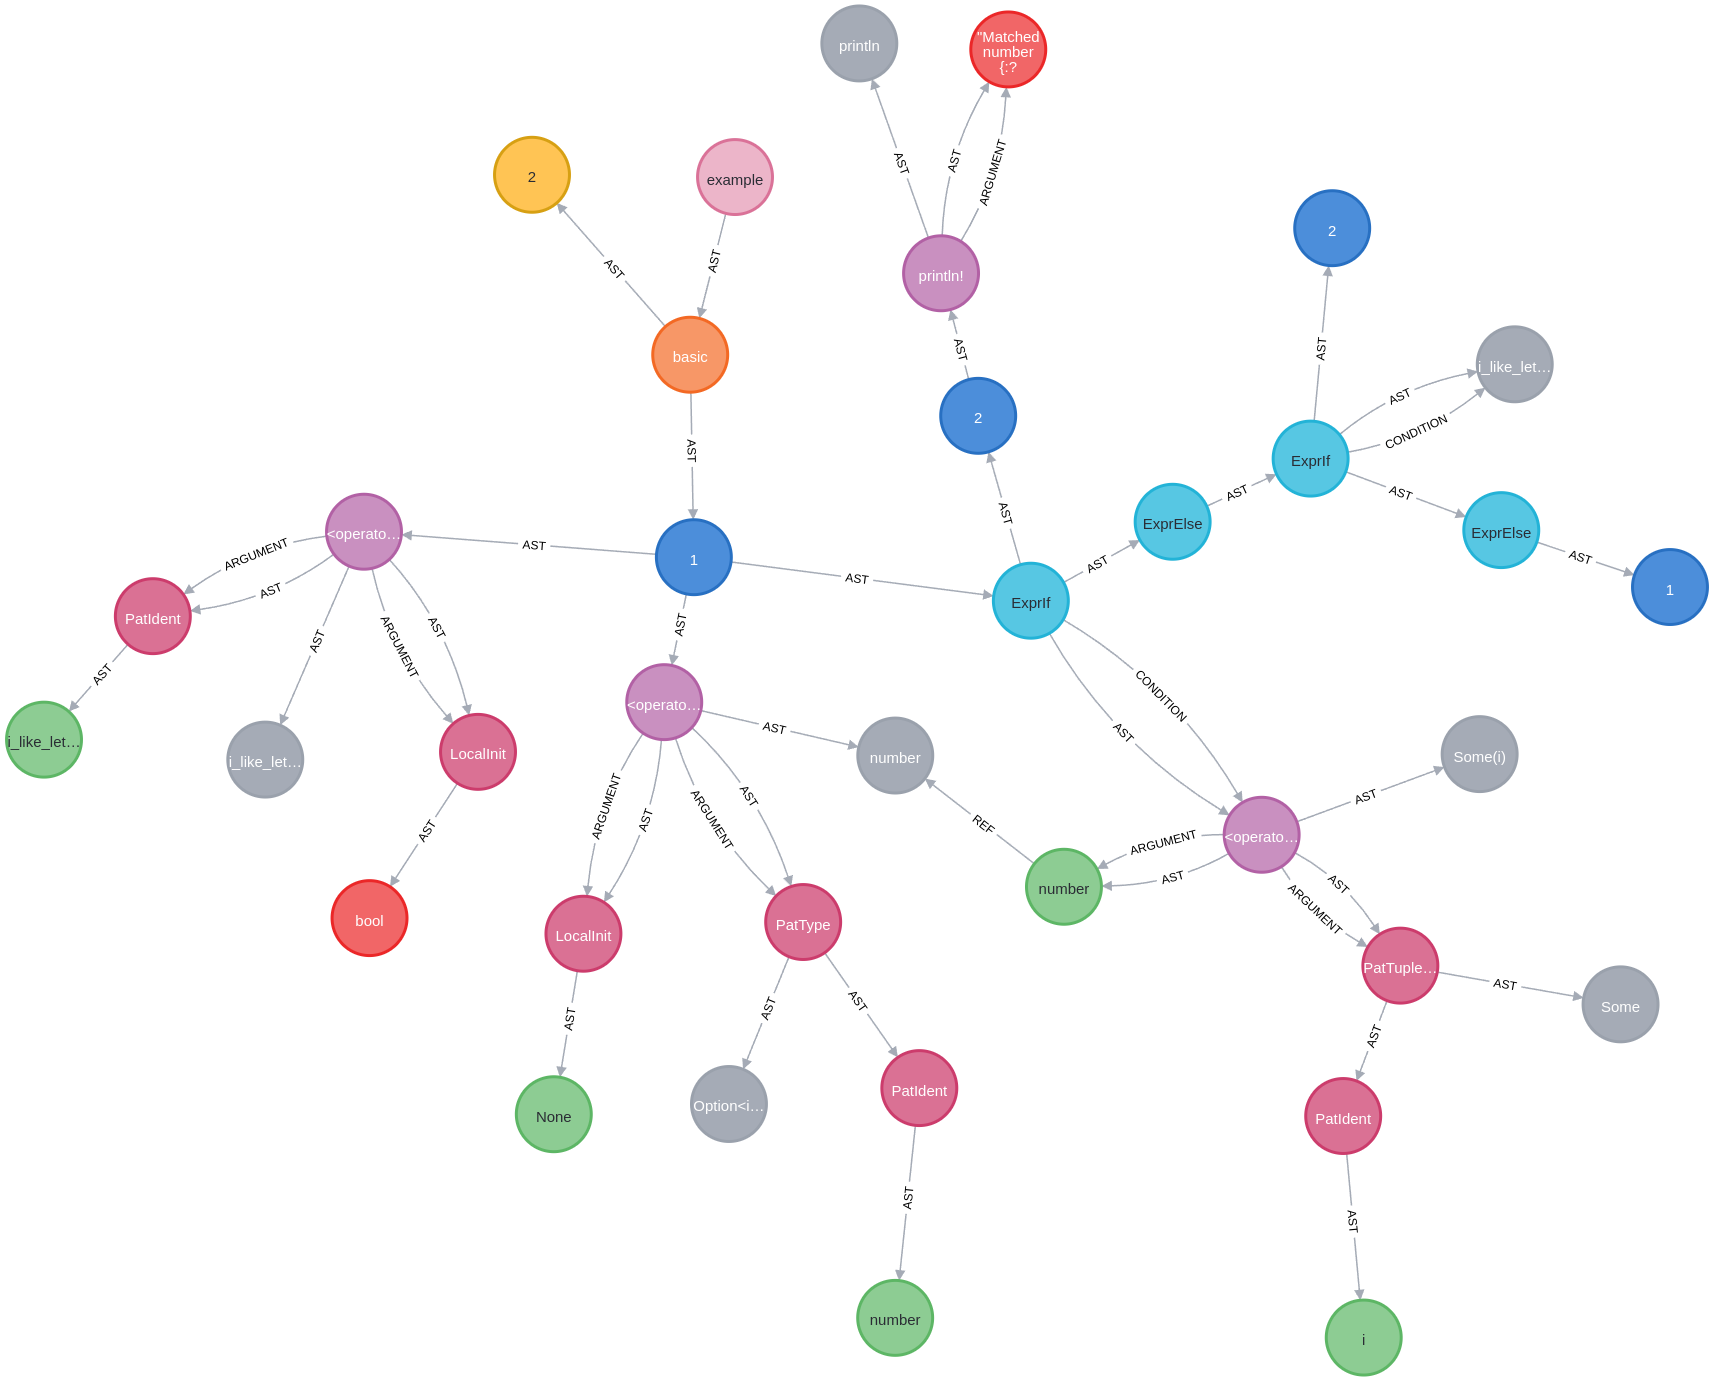
\includegraphics[width=1\columnwidth]{figures/c4/c4_iflet.png}
\centering
\caption{Ví dụ đồ thị CPG cho đoạn mã nguồn của cú pháp if let \ref{code:c4_iflet}.}
\label{img:c4_cpg_iflet}
\end{figure}

% Trong Hình \ref{img:c4_cpg_iflet}, cạnh \texttt{CONDITION} của nút \texttt{ExprIf} trỏ tới nút \texttt{Assignment}, đồng thời cũng khai báo biến mới với tên \texttt{i}. Mặc định, Joern sẽ không cho phép cạnh \texttt{CONDITION} trỏ tới nút \texttt{Assignment} bởi vì trong ngôn ngữ C/C++ không thể lấy một phép gán làm điều kiện. Tuy nhiên, khóa luận đã thực hiện chỉnh sửa đặc tả CPG của Joern để cho phép cạnh \texttt{CONDITION} trỏ tới nút \texttt{Assignment} trong trường hợp này.
% Điều chỉnh này giúp mô hình hóa chính xác hơn ngữ nghĩa của các ngôn ngữ hỗ trợ khai báo biến trực tiếp trong khối điều kiện, như Rust. Các mệnh đề trong khối điều kiện đúng được thực thi, nếu có sử dụng tới biến \texttt{i} thì sẽ tham chiếu tới biến \texttt{i} vừa được khai báo thông qua cạnh \texttt{REF}. Nhờ đó, đồ thị CPG không chỉ phản ánh chính xác cấu trúc mã nguồn mà còn đảm bảo khả năng truy vấn và phân tích đúng các phụ thuộc dữ liệu trong các ngữ cảnh tương tự.

Trong Hình \ref{img:c4_cpg_iflet}, cạnh \texttt{CONDITION} của nút \texttt{ExprIf} trỏ tới nút \texttt{Assignment}, đồng thời cũng khai báo biến mới với tên \texttt{i}.
Mặc định, Joern sẽ không cho phép cạnh \texttt{CONDITION} trỏ tới nút \texttt{Assignment} bởi vì trong ngôn ngữ C/C++ không thể lấy một phép gán làm điều kiện.
Tuy nhiên, khóa luận đã thực hiện chỉnh sửa đặc tả CPG của Joern để cho phép cạnh \texttt{CONDITION} trỏ tới nút \texttt{Assignment} trong trường hợp này.
Điều chỉnh này giúp mô hình hóa chính xác hơn ngữ nghĩa của các ngôn ngữ hỗ trợ khai báo biến trực tiếp trong khối điều kiện như Rust.
Các mệnh đề trong khối điều kiện đúng được thực thi, nếu có sử dụng tới biến \texttt{i} thì sẽ tham chiếu tới biến \texttt{i} vừa được khai báo thông qua cạnh \texttt{REF}.

\subsection{Cú pháp while let}

% Tương tự với tính năng if let ở trên, Rust cũng hỗ trợ việc khai báo biến làm điều kiện cho vòng lặp while.
% Cú pháp của vòng lặp while let như sau:

% \begin{minted}[mathescape, breaklines, frame=lines, framesep=2mm, baselinestretch=1.2, fontsize=\footnotesize, linenos]{rust}
% while let <pattern> = <expression> {
%         <block>
% }
% \end{minted}


\begin{listing}[H]
\begin{minted}[mathescape, breaklines, frame=lines, framesep=2mm, baselinestretch=1.2, fontsize=\footnotesize, linenos]{rust}
let mut optional = Some(0);

while let Some(i) = optional {
    if i > 9 {
        optional = None;
    } else {
        optional = Some(i + 1);
    }
}
\end{minted}
\caption{Ví dụ mã nguồn cho cú pháp while let.}
\label{code:c4_whilelet}
\end{listing}

Tương tự với cú pháp if let ở trên, Rust cũng hỗ trợ việc khai báo biến làm điều kiện cho vòng lặp while.
Đoạn mã \ref{code:c4_whilelet} trên được hiểu là nếu biến \texttt{optional} có giá trị bên trong thì thực hiện vòng lặp, nếu không thì kết thúc vòng lặp.
Đồng thời, sẽ có một biến \texttt{i} mới được khởi tạo đối với mỗi lần lặp, giá trị của \texttt{i} bằng giá trị của số nguyên bên trong biến \texttt{optional}.
Các mệnh đề trong khối được thực thi, và nếu có sử dụng tới, chúng sẽ tham chiếu tới biến \texttt{i} vừa được khai báo thông qua cạnh \texttt{REF}.
Không chỉ vậy, vế phải của điều kiện có thể được gán lại liên tục trong quá trình lặp, đảm bảo vòng lặp kiểm tra trạng thái mới của biến \texttt{optional} sau mỗi lần lặp.
Nhờ vậy thể hiện được các thay đổi động của dữ liệu trong suốt quá trình thực thi vòng lặp.
Khi việc kiểm tra giá trị số nguyên bên trong biến \texttt{optional} thất bại, vòng lặp sẽ kết thúc.
% , đảm bảo hành vi nhất quán với ngữ nghĩa của mã nguồn Rust.

Hình \ref{img:c4_cpg_whilelet} mô tả đồ thị CPG cho đoạn mã nguồn while let ở trên.
Nút \texttt{CONTROL STRUCTURE} thể hiện vòng lặp while, trong khi nút \texttt{ASSIGNMENT} biểu diễn điều kiện của vòng lặp và được nối với nút \texttt{CONTROL STRUCTURE} thông qua cạnh \texttt{CONDITION}
Ngoài ra, biến \texttt{i} được khai báo riêng tại nút \texttt{LOCAL} và tham chiếu thông qua cạnh \texttt{REF} bởi các nút tương ứng với các mệnh đề trong khối mã.

\begin{figure}[H]
    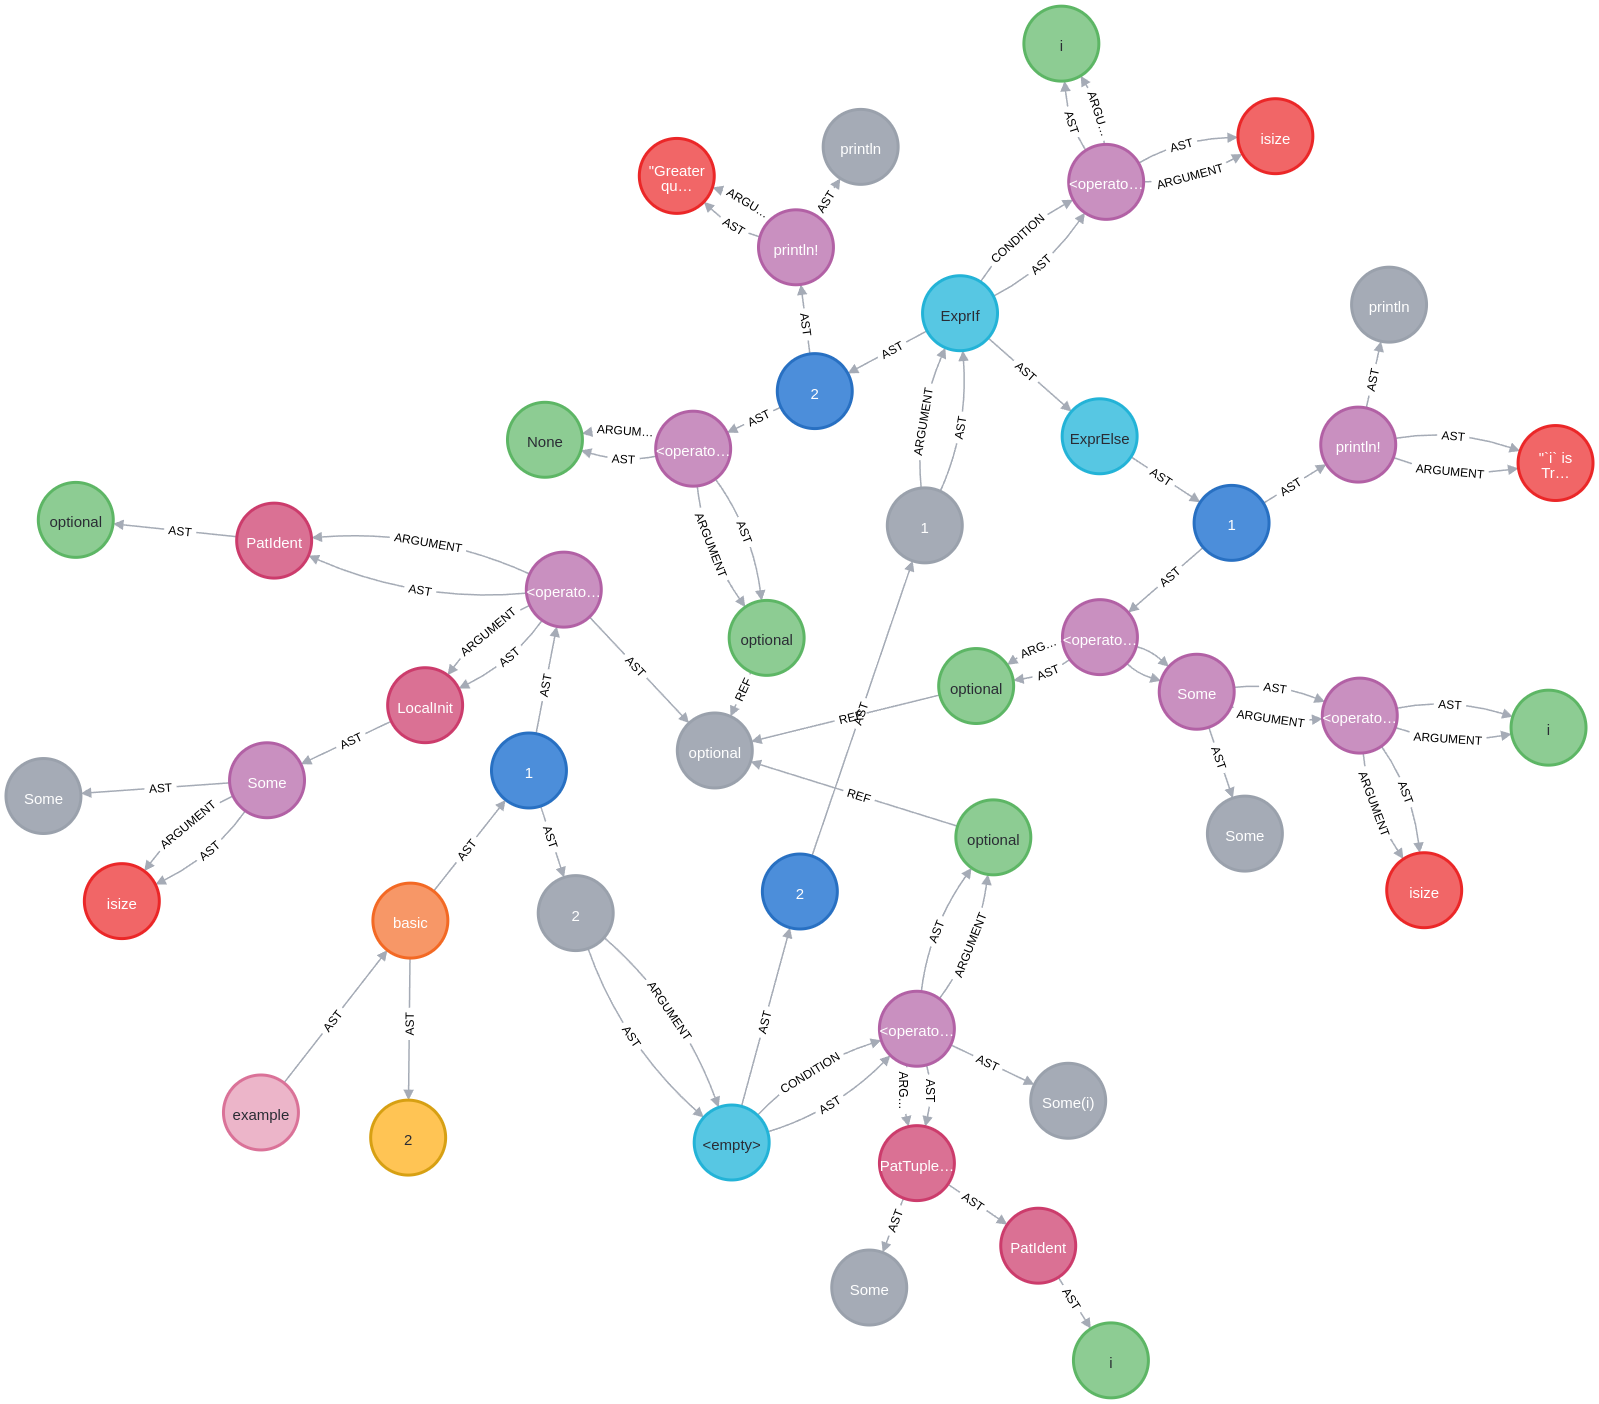
\includegraphics[width=1\columnwidth]{figures/c4/c4_whilelet.png}
    \centering
    \caption{Ví dụ đồ thị CPG cho đoạn mã nguồn cú pháp while let \ref{code:c4_whilelet}.}
    \label{img:c4_cpg_whilelet}
\end{figure}

\subsection{Cú pháp match}

Ngoài việc sử dụng mệnh đề gán biến thành biểu thức điều kiện, tính hướng hàm của Rust còn thể hiện ở sự kết hợp giữa cơ chế pattern matching và kiểu dữ liệu đại số.
Ví dụ \ref{code:c4_match} cho thấy cấu trúc match không chỉ kiểm tra giá trị mà còn kết hợp với các mẫu phức tạp, bao gồm kiểm tra điều kiện, kiểm tra các kiểu dữ liệu khác nhau và so sánh.
Điều này mang lại cho Rust tính linh hoạt cao hơn so với switch trong C/C++ khi chỉ so sánh giá trị nguyên thủy.
Một điểm khác biệt quan trọng giữa match và switch là tính toàn diện của match.
Rust yêu cầu các mẫu trong match phải bao quát tất cả các khả năng có thể xảy ra, nếu không trình biên dịch sẽ báo lỗi.
Điều này giúp đảm bảo rằng không có tình huống nào bị bỏ qua, tăng cường độ an toàn của mã nguồn.
Trong khi đó, switch trong C/C++ không yêu cầu bao quát tất cả các trường hợp, và việc bỏ sót một trường hợp có thể dẫn đến lỗi hoặc hành vi không mong muốn.
Thêm vào đó, match trong Rust cho phép trích xuất và xử lý các thành phần của cấu trúc dữ liệu phức tạp ngay trong quá trình đối chiếu mẫu.
% Ví dụ, Rust có thể match trên \texttt{tuple}, \texttt{enum}, \texttt{struct}, trong khi switch của C/C++ thường chỉ giới hạn trong các giá trị nguyên thủy.
Cú pháp match có thể thực hiện trên \texttt{tuple}, \texttt{enum}, \texttt{struct}, trong khi switch của C/C++ chỉ giới hạn cho các giá trị nguyên thủy.

\begin{listing}[H]
\begin{minted}[mathescape, breaklines, frame=lines, framesep=2mm, baselinestretch=1.2, fontsize=\footnotesize, linenos]{rust}
enum Color {
    Red,
    Blue(u32, u32, u32),
    Green {
        red: u32,
        green: u32,
        blue: u32,
    },
}

fn main() {
    let color = Color::Blue(0, 0, 255);

    match color {
        Color::Red =>
            println!("The color is Red!")
        Color::Blue(r, g, b) =>
            println!("R: {}, G: {}, B: {}!", r, g, b)
        Color::Green {red, green, blue} =>
            println!("R: {}, G: {}, B: {}!", red, green, blue),
    }
}
\end{minted}
\caption{Ví dụ mã nguồn cho cú pháp match.}
\label{code:c4_match}
\end{listing}

Trong Hình \ref{img:c4_match}, các biến thể của \texttt{enum Color} được thể hiện bằng nút \texttt{VARIANT}.
Biến thể \texttt{Red} do không có giá trị nên không có nút con nào khác.
Biến thể \texttt{Blue} có giá trị là 3 số nguyên tính theo chỉ mục nên sẽ có 3 nút con \texttt{MEMBER} tương ứng, nhưng mỗi nút \texttt{MEMBER} này không có nút con \texttt{IDENTIFIER} chỉ ra tên thành phần.
Ngược lại mỗi nút \texttt{MEMBER} của \texttt{Green} sẽ có nút con \texttt{IDENTIFIER} thể hiện tên của thành phần.
Còn cú pháp match được thể hiện bằng nút \texttt{CONTROL STRUCTURE} và cạnh \texttt{CONDITION} nối với nút \texttt{IDENTITER} chi tới biến \texttt{color}.
Mỗi trường hợp của match sẽ được thể hiện bằng nút \texttt{ARM} và mỗi \texttt{ARM} cũng có sẽ cạnh \texttt{CONDITION} nối tới nút thể hiện biểu thức điều kiện.

\begin{figure}[H]
    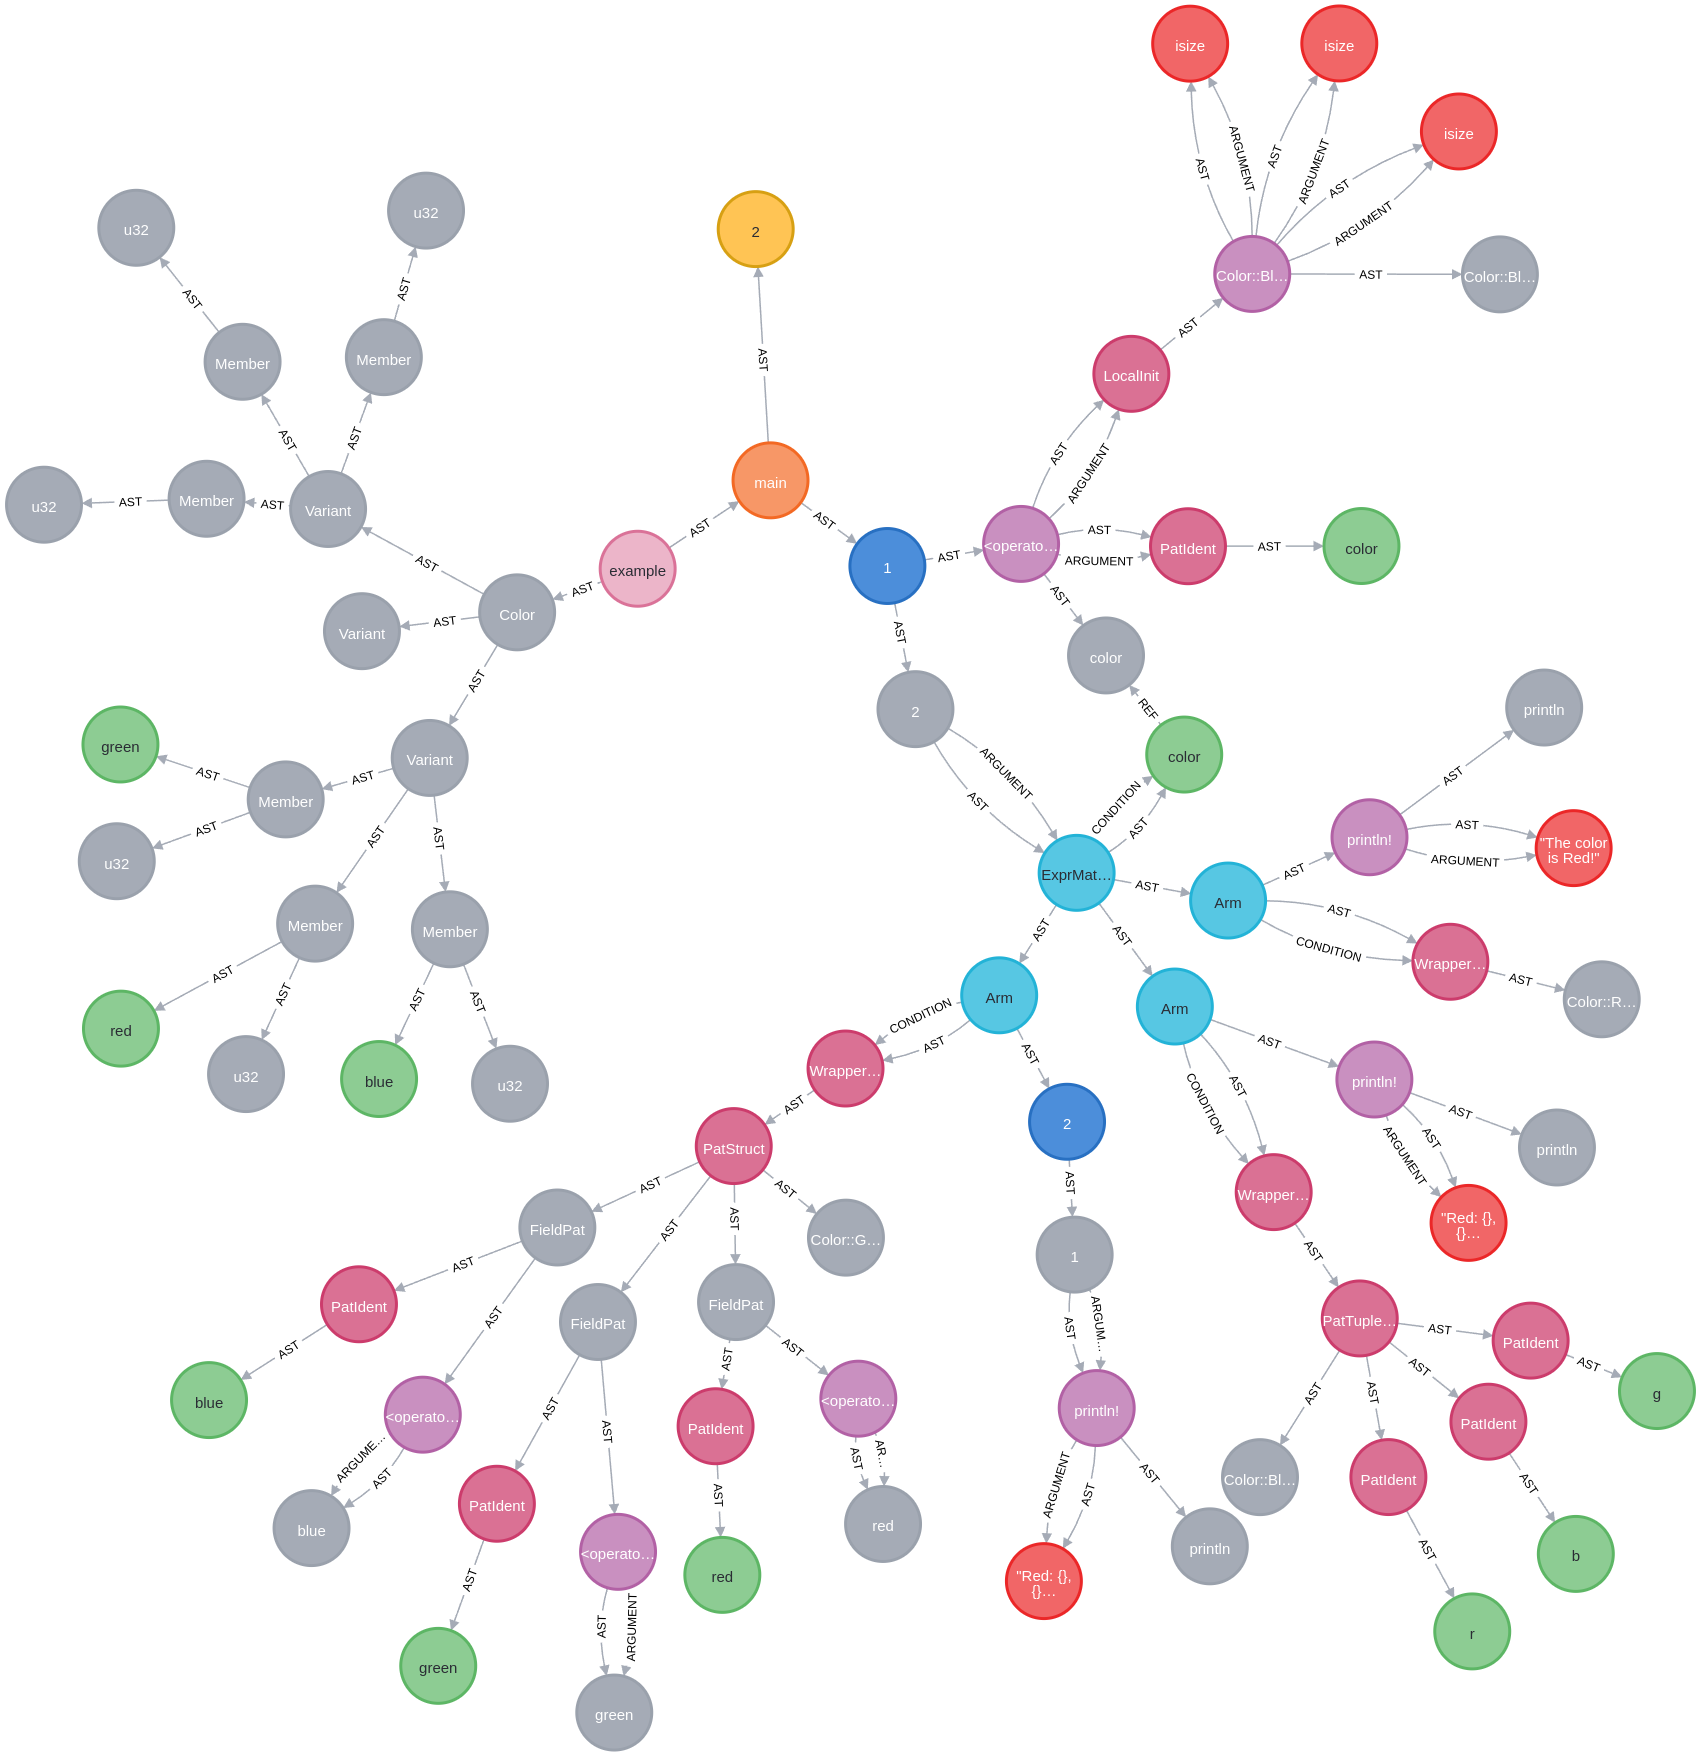
\includegraphics[width=1\columnwidth]{figures/c4/c4_match.png}
    \centering
    \caption{Ví dụ đồ thị CPG cho đoạn mã nguồn cú pháp match \ref{code:c4_match}.}
    \label{img:c4_match}
\end{figure}

\subsection{Cú pháp lifetime}

Lifetime là cơ chế được sử dụng trong Rust để quản lý vòng đời của các biến tham chiếu.
Quản lý lifetime một cách chặt chẽ đảm bảo rằng các biến tham chiếu không trỏ tới vùng nhớ không còn tồn tại.
Lifetime có vai trò tương tự như kiểu tổng quát, nhưng thay vì định kiểu cho biến thì lifetime sẽ xác định thời gian hợp lệ cho biến tham chiếu.
Để biểu diễn được kiểu dữ liệu tổng quát, đặc tả CPG của Joern đã có các nút như \texttt{TYPE}, \texttt{TYPE PARAMETER}, \texttt{TYPE ARGUMENT}.
Do vậy để biểu diễn được tính năng lifetime trên đồ thị CPG, 3 loại nút mới đã được thêm vào đặc tả CPG bao gồm \texttt{LIFETIME}, \texttt{LIFETIME PARAMETER}, \texttt{LIFETIME ARGUMENT}.
Để chỉ ra quan hệ ràng buộc giữa biến và lifetime hay quan hệ giữa các lifetime với nhau, ta sẽ thêm cạnh \texttt{OUT LIVE}.
Cạnh \texttt{OUT LIVE} mang ý nghĩa nút nguồn phải có thời gian hợp lệ lớn hơn nút đích. Quy định về thời gian hợp lệ của một đơn vị thành phần so với đơn vị thành phần khác được tham khảo từ Rust Reference.

Nút \texttt{LIFETIME PARAMETER} và \texttt{LIFETIME ARGUMENT} được sử dụng cho các \texttt{struct}, \texttt{enum}, \texttt{trait} để chỉ ra lifetime tổng quát cho các biến tham chiếu.
Loại nút \texttt{LIFETIME} sẽ thể hiện vòng đời thực sự của biến tham chiếu.
Các biến tham chiếu sẽ được gán lifetime thông qua việc sử dụng dấu "\texttt{'}" đi trước tên lifetime, ví dụ như \texttt{'a}.
Nếu biến đánh dấu lifetime \texttt{'a} thì sẽ có cạnh \texttt{OUT LIVE} trỏ từ nút \texttt{IDENTIFIER} của biến tới nút \texttt{LIFETIME} đại diện cho \texttt{'a} tương ứng.
Nếu lifetime \texttt{'a} được giới hạn bởi lifetime \texttt{'b} thì sẽ có cạnh \texttt{OUT LIVE} từ nút \texttt{LIFETIME} \texttt{'a} tới nút \texttt{LIFETIME} \texttt{'b}.

% Lifetime elision là cơ chế trong Rust giúp tự động suy diễn lifetime cho các biến tham chiếu.
% Có ba luật chính về lifetime elision trong Rust.
% Thứ nhất, mỗi biến tham chiếu đầu vào sẽ được tự động gán lifetime mà không cần phải đánh dấu một cách tường minh.
% Thứ hai, nếu hàm có chỉ có một biến tham chiếu đầu và một biến tham chiếu đầu ra, trình biên dịch sẽ suy luận rằng biến tham chiếu đầu ra có cùng lifetime với biến tham chiếu đầu vào.
% Cuối cùng, nếu hàm có một hoặc nhiều hơn một biến tham chiếu đầu vào và một trong biến đầu vào là biến \texttt{self} (\texttt{self} tương đương với \texttt{this} trong C/C++), trình biên dịch sẽ suy luận rằng biến tham chiếu đầu ra có cùng lifetime với \texttt{self}.
% Ngoài 3 trường hợp trên, Rust yêu cầu phải ghi rõ lifetime cho tất cả các biến tham chiếu để tránh nhầm lẫn và đảm bảo an toàn bộ nhớ.

\begin{listing}[H]
\begin{minted}[mathescape, breaklines, frame=lines, framesep=2mm, baselinestretch=1.2, fontsize=\footnotesize, linenos]{rust}
fn longest<'a>(x: &'a str, y: &'a str) -> &'a str {
    if x.len() > y.len() {
        x
    } else {
        y
    }
}
\end{minted}
\caption{Ví dụ mã nguồn cho lifetime.}
\label{code:c4_lifetime_1}
\end{listing}

Các biến tham chiếu luôn có một lifetime tương ứng với nó, có thể được chỉ ra tường minh hoặc không tường minh.
Đoạn mã \ref{code:c4_lifetime_1} mô tả một ví dụ bắt buộc phải khai báo lifetime một cách tường minh để chỉ rõ vòng đời của biến tham chiếu.
Hàm \texttt{longest} nhận vào 2 biến tham chiếu \texttt{x} và \texttt{y} cùng có lifetime \texttt{'a} và giá trị trả về cũng có lifetime \texttt{'a}.
Trình biên dịch Rust có thể tự động suy diễn lifetime không tường minh cho hai biến tham chiếu đầu vào \texttt{x} và \texttt{y}, nhưng không thể suy diễn được lifetime cho giá trị tham chiếu trả về.
Hơn nữa, giá trị trả về của hàm \texttt{longest} là một trong hai giá trị tham chiếu đầu vào.
Do trình biên dịch không thể biết được trong khi thực thi hàm thì giá trị trả về sẽ trỏ tới vùng nhớ của \texttt{x} hay \texttt{y}, do đó cần phải chỉ rõ lifetime cho giá trị trả về.
Biến \texttt{x} và \texttt{y} cùng có lifetime \texttt{'a} tức là \texttt{x} và \texttt{y} sẽ có một khoảng thời gian mà \texttt{x} và \texttt{y} cùng tồn tại và đặt tên khoảng thời gian đó là \texttt{'a}.
Giá trị đầu ra tồn tại trong khoảng thời gian \texttt{'a} này thì luôn đảm bảo không trỏ tới vùng nhớ không còn tồn tại.
Khi sử dụng hàm, nếu đối số đầu vào hay biến nhận giá trị trả về không thỏa mãn ràng buộc lifetime \texttt{'a} thì trình biên dịch Rust sẽ báo lỗi.

\vspace{\baselineskip}

\begin{figure}[H]
    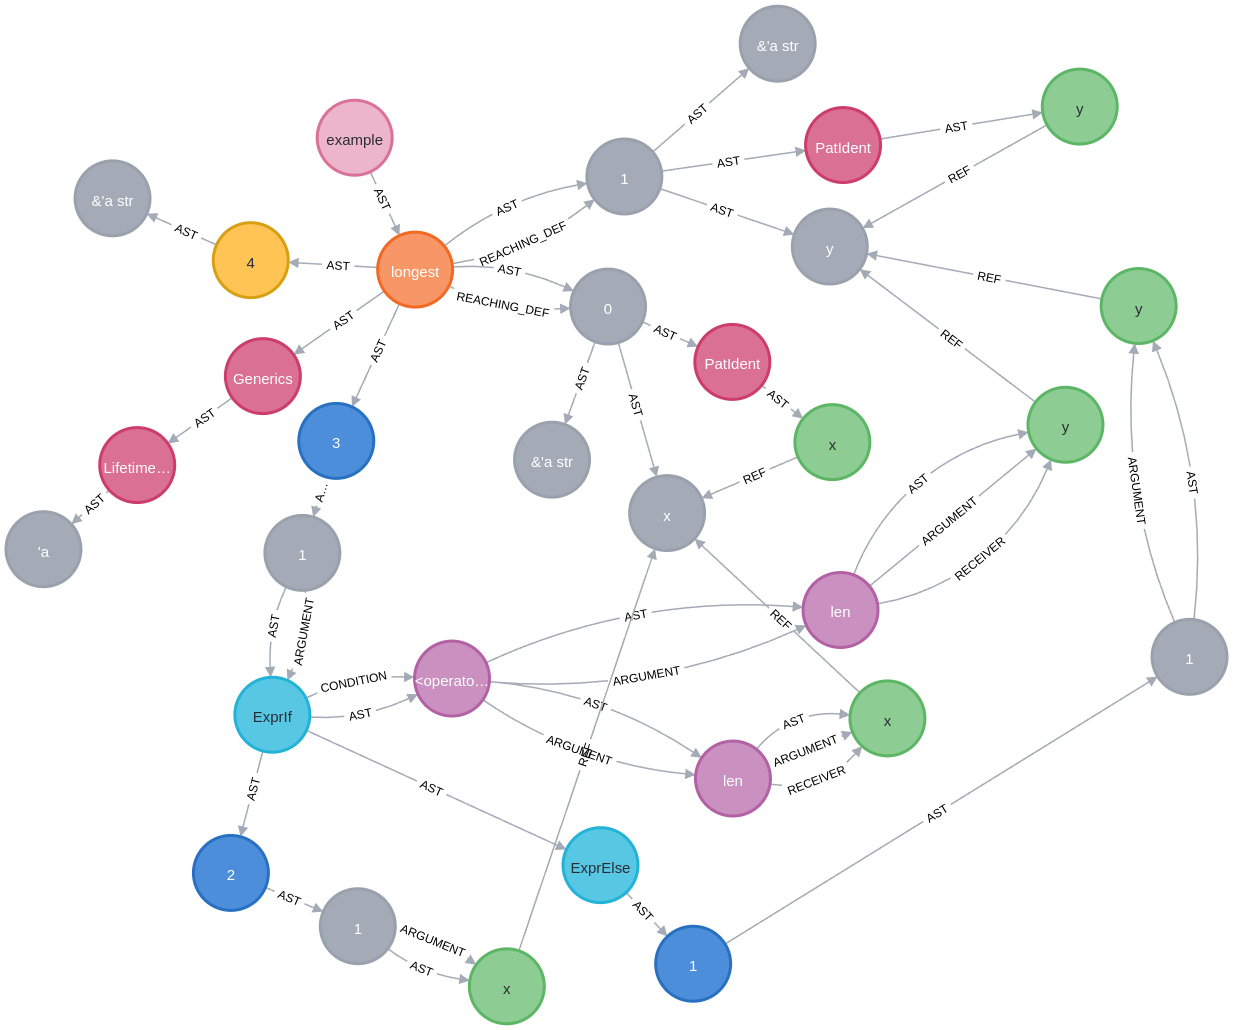
\includegraphics[width=1\columnwidth]{figures/c4/c4_lifetime_1.png}
    \centering
    \caption{Ví dụ đồ thị CPG cho đoạn mã nguồn \ref{code:c4_lifetime_1}.}
    \label{img:c4_lifetime_1}
\end{figure}

Hình \ref{img:c4_lifetime_1} thể hiện mối quan hệ lifetime giữa các biến tham chiếu và giá trị trả về của hàm.
Hàm \texttt{longest} được thể hiện qua nút \texttt{METHOD}.
Trong đó, nút \texttt{METHOD} có cạnh \texttt{AST} trỏ tới nút \texttt{GENERICS}, đại diện cho nút cha bọc lấy nhiều nút thể hiện kiểu tổng quát.
Nút \texttt{LIFETIME PARAMETER} thể hiện lifetime \texttt{'a} của hàm, và cũng là lifetime của các biến tham chiếu và giá trị trả về.
Các biến tham chiếu \texttt{x} và \texttt{y} có cùng lifetime \texttt{'a} được thể hiện qua cạnh \texttt{OUT LIVE} từ nút \texttt{IDENTIFIER} của biến \texttt{x} và \texttt{y} tới nút \texttt{LIFETIME} của \texttt{'a}.
Giá trị trả về của hàm cũng có lifetime \texttt{'a} và được thể hiện qua cạnh \texttt{OUT LIVE} từ nút \texttt{METHOD RETURN} tới nút \texttt{LIFETIME} \texttt{'a}.
Mối quan hệ lifetime giữa các biến tham chiếu và giá trị trả về đều được thể hiện qua các nút \texttt{LIFETIME} và cạnh \texttt{OUT LIVE} trên đồ thị CPG.

\begin{listing}[H]
\begin{minted}[mathescape, breaklines, frame=lines, framesep=2mm, baselinestretch=1.2, fontsize=\footnotesize, linenos]{rust}
fn f<'a, 'b, 'c, T>(x: &'a i32, mut y: &'b i32, z: &'c T)
where
    'b: 'a,
    'c: 'b,
    T: 'b,
{
    // ...
}
\end{minted}
\caption{Ví dụ mã nguồn cho cú pháp lifetime kết hợp cú pháp where.}
\label{code:c4_lifetime_2}
\end{listing}


\begin{figure}[H]
    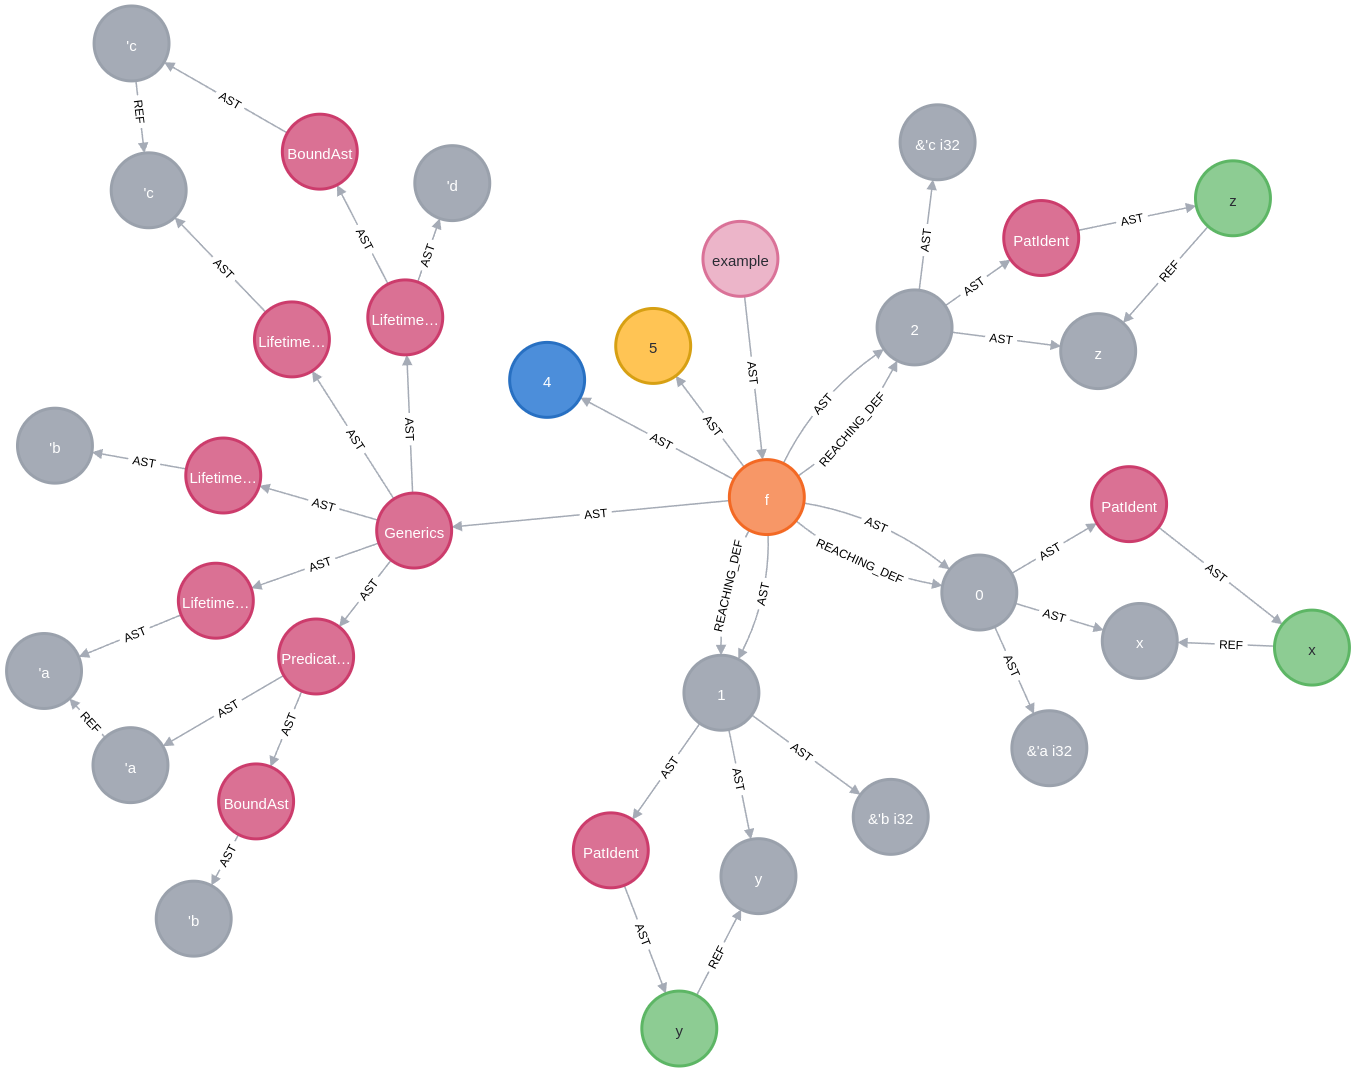
\includegraphics[width=1\columnwidth]{figures/c4/c4_lifetime_2.png}
    \centering
    \caption{Ví dụ đồ thị CPG cho đoạn mã nguồn cú pháp where \ref{code:c4_lifetime_2}.}
    \label{img:c4_lifetime_2}
\end{figure}

Trong Rust, kiểu tổng quát và ràng buộc của nó có thể được chỉ rõ thông qua cú pháp \texttt{where}.
Cú pháp \texttt{where} cho phép thể hiện ràng buộc giữa kiểu dữ liệu tổng quát và kiểu lifetime tổng quát.
Đoạn mã \ref{code:c4_lifetime_2} minh họa về một hàm có nhiều lifetime, nhiều kiểu tổng quát và tham chiếu đầu vào kết hợp với cú pháp \texttt{where} để thể hiện mối quan hệ ràng buộc giữa chúng.
Hàm \texttt{f} nhận vào 3 biến tham chiếu \texttt{x}, \texttt{y}, \texttt{z} có lifetime tương ứng là \texttt{'a}, \texttt{'b}, \texttt{'c}.
Cú pháp \texttt{'b: 'a} thể hiện ràng buộc lifetime \texttt{'b} của biến \texttt{y} phải lớn hơn hoặc bằng lifetime \texttt{'a} của biến \texttt{x}.
Trên đồ thị CPG ở Hình \ref{img:c4_lifetime_2}, điều này tức là sẽ có cạnh \texttt{OUT LIVE} từ nút \texttt{LIFETIME} \texttt{'b} tới nút \texttt{LIFETIME} \texttt{'a}.
Điều này tương tự với việc lifetime \texttt{'c} của biến \texttt{z} phải lớn hơn hoặc bằng lifetime \texttt{'b} của biến \texttt{y}.
Cạnh \texttt{OUT LIVE} từ nút \texttt{LIFETIME} \texttt{'c} tới nút \texttt{LIFETIME} \texttt{'b} được thể hiện rõ ràng trên đồ thị CPG.

Không chỉ ràng buộc giữa các lifetime với nhau, hoàn toàn có thể ràng buộc lifetime cho một kiểu dữ liệu tổng quát.
Kiểu dữ liệu \texttt{T} của biến \texttt{y} phải có lifetime lớn hơn \texttt{'b} thông qua cú pháp \texttt{T: 'b}.
Cú pháp này sẽ có ý nghĩa trong trường hợp khi T là một kiểu \texttt{struct} tự định nghĩa, thì tất cả các thuộc tính tham chiếu của T cũng phải có lifetime lớn hơn hoặc bằng \texttt{'b}.
Sẽ có cạnh \texttt{LIFETIME} từ nút \texttt{TYPE} của kiểu \texttt{T} tới nút \texttt{LIFETIME} \texttt{'b} để thể hiện mối quan hệ ràng buộc giữa chúng.
Rust cung cấp hai cách để thể hiện ràng buộc cho kiểu dữ liệu và kiểu lifetime tổng quát.
Một là khai báo ngay tại phần khai báo hàm, hai là sử dụng cú pháp \texttt{where} để thể hiện ràng buộc.
Lưu ý rằng khai báo ngay tại hàm và cú pháp \texttt{where} không thay thế cho nhau mà cùng tồn tại để có thể kết hợp với nhau.
Khai báo ngay tại hàm mang ý nghĩa khai báo nên sẽ sử dụng các nút \texttt{TYPE PARAMETER} và \texttt{LIFETIME PARAMETER} để thể hiện.
Còn cú pháp \texttt{where} mang ý nghĩa ràng buộc nên sẽ sử dụng các nút \texttt{TYPE}, \texttt{LIFETIME} và cạnh \texttt{OUT LIVE}.

Ownership, borrowing và lifetime là 3 tính năng làm nên cơ chế an toàn bộ nhớ trong Rust.
Đây là bộ ba tính năng quan trọng làm cho Rust trở nên khác biệt so với các ngôn ngữ lập trình khác.
Đồ thị CPG cần phải thể hiện được 3 tính năng trên và cung cấp thông tin thông qua các nút, cạnh và thuộc tính phù hợp.
Đặc biệt là tính năng lifetime thể hiện sự hợp lệ của các biến tham chiếu.
Do đó việc thể hiện đúng quan hệ giữa lifetime và biến, lifetime với lifetime, biến với biến là rất quan trọng.
Từ đó có thể khai thác thông tin để kiểm tra sự hợp lệ của biến tham chiếu, giúp phát hiện được các lỗi về bộ nhớ gây ra khi đánh dấu lifetime không chính xác.

\section{Hạn chế}

\subsection{Chưa hỗ trợ cú pháp Macro}

Trong ngôn ngữ lập trình C/C++ và Rust có tính năng macro, là cách viết mã nguồn để sinh ra mã nguồn khác \cite{rustlangMacrosRust}.
% Macro trong Rust bao gồm 2 loại declarative macro và procedural macro.
% Declarative macro giống như macro trong C/C++ \cite{}, còn procedural macro giống như inline function.
Ngôn ngữ C/C++ có bộ tiền xử lý trước khi cho mã nguồn vào trình biên dịch, đo đó sau khi được tiền xử lý thì mã nguồn đã được xử lý toàn bộ macro.
Tuy nhiên, Rust không giống C/C++, macro của Rust không được xử lý ở trước khi sinh cây AST mà sẽ được xử lý sau khi sinh cây AST nhưng trước khi đi vào pha phân tích ngữ cảnh của trình biên dịch \cite{veykrilSourceAnalysis}.
Như đã đề cập ở phần các trước, công cụ hiện tại sử dụng thư viện syn để sinh cây AST cho mã nguồn và syn không hỗ trợ xử lý macro.
Do đó tất cả các mã lệnh nằm bên trong macro sẽ không được xử lý, dẫn đến việc không thể sinh cây AST cho đoạn mã lệnh sử dụng macro.
Tất cả các đoạn lệnh nằm trong một lời gọi macro hiện tại được xem như một chuỗi ký tự.
Không chỉ vậy macro trong Rust sử dụng DSL (Domain-Specific Language) riêng, DSL này gần với ngôn ngữ Rust nhưng có sự mở rộng biến đổi để phù hợp với vai trò macro, do đó không thể sinh cây AST cho macro.

Để xử lý trường hợp trên, một bước tiền xử lý mã nguồn có thể được thêm vào để mở rộng macro như C/C++.
Công cụ có thể sử dụng đến tính năng mở rộng marco của trình biên dịch Rust \cite{rustlangMacroExpansion}.
Tính năng này có tác dụng đưa đoạn mã macro mà lập trình viên nhìn thấy thành đoạn mã mà trình biên dịch nhìn thấy.
Mã nguồn sau khi được mở rộng sẽ thay thế các lời gọi macro bằng định nghĩa gốc của macro.
Các macro nạp sẵn của ngôn ngữ Rust như \texttt{println!}, \texttt{vec!} hay kể cả macro do người dùng định nghĩa cũng sẽ được xử lý.
Không chỉ vậy, mã nguồn sau khi được mở rộng thì sẽ có được các thông tin bị ẩn đi như các mặc định của Rust bao gồm các hàm, các ký tự được nạp sẵn trong ngôn ngữ.
Tuy nhiên, việc mở rộng macro trước khi cho vào sinh cây AST sẽ làm cho mã nguồn bị biến đổi so với mã nguồn gốc, đồng thời tăng kích cỡ và độ lớn của mã nguồn.
Việc thêm các thông tin ẩn mà lập trình viên không nhìn thấy có thể gây nhầm lẫn.
Điều này cũng đồng nghĩa với việc quá trình sinh cây AST cho mã nguồn sau khi xử lý macro sẽ phức tạp và tốn nhiều thời gian hơn.

\subsection{Chưa hỗ trợ cơ chế Module}

Cơ chế module trong Rust tương tự namespace trong C++, package trong Java \cite{rustlangManagingGrowing}.
Module chia nhỏ mã nguồn thành các phần nhỏ hơn, tổ chức và quản lý mã nguồn, giúp tái sử dụng mã nguồn, giúp tránh xung đột tên biến, hàm giữa các module khác nhau.
Một module trong Rust có thể là một tệp riêng biệt hoặc nằm chung trong một tệp mã nguồn.
Các module có thể được tổ chức thành một hệ thống phân cấp, với các module con được khai báo bên trong các module cha.
% Có một số tệp được coi là tệp đặc biệt trong cấu trúc mã nguồn trong rust.
% Ví dụ như tệp mod.rs, đây là tệp module gốc của thư mục chứa nó, tất cả các module con trong thư mục đó sẽ được import thông qua module gốc mod.rs.
% Ngoài ra còn có tệp main.rs, lib.rs để đánh dấu điểm đầu vào của chương trình và xác định xem dự án là một thư viện hay một ứng dụng.
Rust còn cung cấp cơ chế workspace, cho phép quản lý nhiều dự án nhỏ trong cùng một dự án lớn, mỗi dự án là một thư mục con trong thư mục gốc lớn nhất \cite{rustlangCargoWorkspaces}.
Để kiểm soát khả năng truy cập, Rust sử dụng cơ chế visibility \cite{rustlangVisibilityPrivacy}.
Mặc định các thành phần trong module chỉ có phạm vi truy cập giới hạn trong module nó được định nghĩa.
Để làm cho một đơn vị có thể truy cập được từ các module khác, ta sử dụng từ khóa \texttt{pub} đơn vi cần mở rộng truy cập.
Ngoài ra, Rust có cơ chế đường dẫn dùng để định danh một thành phần cấu trúc từ module khác ta mà ta có thể truy cập nếu cho phép.
Một đường dẫn có thể là đường dẫn tuyệt đối hoặc đường dẫn tương đối.
Ví dụ dùng từ khóa \texttt{self} để chỉ tới module hiện tại, từ khóa \texttt{super} để chỉ tới module cha của module hiện tại, từ khóa \texttt{crate} để chỉ tới module gốc của dự án.
Hệ thống module phức tạp của Rust làm tăng đáng kể độ khó cho việc xử lý quan hệ giữa các module trong cây AST và phân tích ngữ cảnh.
Các khái niệm như workspace, module, visibility và cơ chế đường dẫn tạo nên sự phức tạp cho việc phân tích mã nguồn, ngữ cảnh của mã nguồn.
Hiện tại công cụ chưa xử lý được các tính năng xung quanh các khái niệm này.

% \subsection{Path}

% \begin{itemize}
%     \item Path có thể là Absolute Path hoặc Relative Path tùy vào bối cảnh module hiện tại, path có thể chỉ tới đối tượng trong cùng một module hoặc khác module
%     \item Path trong Rust là đường dẫn đến một đối tượng nào đó được định nghĩa trong mã nguồn như struct, trait, static, const, function
%     \item Cây AST sử dụng thư viện $syn$, $syn$ có thể lấy được path của một đối tượng nhưng không biết được đối đượng đang trỏ tới là static, const, hay function.
% Do đó đang không phân biệt được đâu là path của static, const, hay function
% \end{itemize}

% \subsection{Type Argument match Type Parameter}

% \subsection{Các lớp thông tin khác của đồ thị CPG}

% Như đã trình bày ở phần kiến trúc của công cụ Joern, một đồ thị CPG sẽ bao gồm nhiều lớp thông tin khác nhau như AST, CFG, PDG hay các lớp thông tin khác của Joern và đặc thù của ngôn ngữ.
% Hiện tại công cụ đã xử lý toàn bộ thông tin của lớp AST, phần lớn các thônng tin của lớp CFG, PDG.
% Tuy nhiên vẫn còn một số lớp thông tin khác phục vụ cho việc duyệt đồ thị, liên kết đồ thị như \texttt{tệpSystem}, \texttt{Shortcuts}, \texttt{TagsAndLocation}, \texttt{Annotation} vẫn chưa được đầy đủ.
% Do vậy, một trong các mục tiêu tương lai của công cụ là hoàn thiện các lớp thông tin này.
\newpage\cleardoublepage
\chapter{Chuyển đổi mã nguồn Rust sang đồ thị CPG}
\label{chap:mapping}

% Chương 4 trình bày về cách ánh xạ cây AST sang đồ thị CPG trên các thể loại cú pháp Rust.
% Mức độ cài đặt và các hạn chế hiện thời của công cụ sẽ được thảo luận.
% Không chỉ vậy, công cụ sẽ được sử dụng để phân tích mã nguồn của một số đoạn mã có lỗ hổng bảo mật được công bố trên RUSTSEC Database \cite{rustsecAboutRustSec}.
% Ngoài ra, chương cũng sẽ thực nghiệm ứng dụng đồ thị CPG trong bài toán học máy phân loại mã nguồn Rust có lỗ hổng bảo mật, thực hiện so sánh với mô hình học máy khác và chứng minh tiềm năng khai thác của đồ thị CPG dành cho ngôn ngữ Rust.

Nội dung của chương 4 là về việc chuyển đổi mã nguồn sang đồ thị CPG trên các thể loại cú pháp Rust.
Mức độ cài đặt của công cụ cho việc bao phủ các loại nút AST và ánh xạ chúng sang nút CPG tương ứng sẽ được thảo luận.
Ngoài ra, chương cũng sẽ trình bày về các hạn chế hiện thời của công cụ.

\section{Mức độ cài đặt công cụ}

Theo thư viện \href{https://docs.rs/syn/2.0.87/syn/}{syn v2.0.87}, phiên bản hiện thời có định nghĩa của 162 struct tương ứng với 162 loại nút AST và 33 enum tương ứng với 33 loại nút AST đa hình.
Hiện tại công cụ đã ánh xạ 162 loại nút AST và 33 loại nút AST đa hình ở trên thành một loại nút CPG tương ứng, tức là 100\% định nghĩa các loại nút AST đã được ánh xạ sang nút CPG.
\href{https://github.com/congnghiahieu/rust-parser/blob/master/docs/MAPPING.md}{Bảng tổng hợp ánh xạ 1-1 nút AST sang nút CPG.}

Công cụ được thực hiện kiểm thử trên 151 tệp mã nguồn bao gồm đa dạng các thể loại cú pháp, thu thập từ trang \href{https://doc.rust-lang.org/stable/rust-by-example/index.html}{Rust By Example} thuộc Rust Foundation \cite{rustlangRustFoundation}.
Ngoài ra, việc chuyển đổi từ AST sang CPG được kiểm tra trên 20 dự án lớn nằm trong 100 dự án Rust có lượng sao lớn nhất trên Github \cite {githubGithubRankingTop100RustmdMaster}.
Mã nguồn của công cụ được lưu trữ tại địa chỉ \href{https://github.com/congnghiahieu/rust-parser}{rust-parser}, \href{https://github.com/congnghiahieu/syn-serde}{syn-serde}, \href{https://github.com/congnghiahieu/joern}{joern}, \href{https://github.com/congnghiahieu/codepropertygraph}{codepropertygraph}.

\section{Các cú pháp đã hỗ trợ}

Phần này sẽ trình bày một số cú pháp của Rust khác biệt so với ngôn ngữ C/C++ và cách mà công cụ đã hỗ trợ cho các cú pháp này.
Các cú pháp bao gồm: if let, while let, match, lifetime.
Những đoạn mã nguồn và hình ảnh mô tả đồ thị CPG được sử dụng từ giờ đến cuối chương đã được đơn giản hóa để dễ dàng thể hiện và minh họa.
Các cạnh và các nút không phải trọng tâm của đồ thị CPG đã được loại bỏ để tập trung vào các tính năng cần trình bày.

\subsection{Cú pháp if let}
If else là cấu trúc điều khiển có mặt trong tất cả các loại ngôn ngữ phổ biến.
Nó cho phép chúng ta kiểm tra một điều kiện và thực thi một khối mã nếu điều kiện đúng và một khối mã khác nếu điều kiện sai.
Cấu trúc câu lệnh if else sẽ bao gồm một điều kiện và 2 khối mã.
Nếu điều kiện đúng, khối mã trong if sẽ được thực thi, ngược lại khối mã trong else sẽ được thực thi.
Thông thường khối điều kiện sẽ là biểu thức trả về kết quả đúng hoặc sai của biểu thức đó.
Trong ngôn ngữ như C/C++ thì chỉ chấp nhận biểu thức điều kiện, việc sử dụng mệnh đề có dấu hai chấm để kết thúc câu lệnh là không hợp lệ.

Với phương châm \textit{"Expression over statement"} và nhằm mục đích tạo sự ngắn gọn, Rust cho phép thực hiện phép khai báo biến và gán giá trị cho biến trong cùng một câu lệnh bằng điều kiện if let.
Cú pháp của câu lệnh if let như sau:

\begin{minted}[mathescape, breaklines, frame=lines, framesep=2mm, baselinestretch=1.2, fontsize=\footnotesize, linenos]{rust}
if let <pattern> = <expression> {
     <block>
} else {
     <block>
}
\end{minted}

\usemintedstyle{default}

Cú pháp này sẽ thực hiện 2 công việc, kiểm tra xem \texttt{<expression>} có khớp với \texttt{<pattern>} hay không, nếu không khớp thì trả về $false$, nếu có khớp thì tiếp tục thực hiện tạo biến mới dựa theo \texttt{<pattern>} vừa lấy được và trả về $true$.
Các biến được khai báo mới từ \texttt{<pattern>} sẽ có phạm vi tồn tại trong khối lệnh điều kiện thành công.
Do thực hiện 2 công việc trong cùng 1 câu lệnh nên khi quy đổi sang câu lệnh tương tự trong ngôn ngữ như C/C++ sẽ tương đương 2 câu lệnh kiểm tra điều kiện và gán biến.

\begin{listing}[H]
\begin{minted}[mathescape, breaklines, frame=lines, framesep=2mm, baselinestretch=1.2, fontsize=\footnotesize, linenos]{rust}
let number: Option<i32> = None;
let i_like_letters = false;

if let Some(i) = number {
    println!("Matched number {:?}!", i);
} else if i_like_letters {
    // ...
} else {
    // ...
}
\end{minted}
\caption{Ví dụ mã nguồn cho if let}
\label{code:c4_iflet}
\end{listing}

\begin{listing}[H]
\begin{minted}[mathescape, breaklines, frame=lines, framesep=2mm, baselinestretch=1.2, fontsize=\footnotesize, linenos]{cpp}
Object* obj = inputObj();

if (obj != nullptr) { // 1 câu lệnh kiểm tra điều kiện
    int number = *static_cast<int*>(obj); // 1 câu lệnh gán biến
    std::cout << "Matched " << number << "!" << std::endl;
}
\end{minted}
\caption{Ví dụ mã nguồn cho if let tương đương trong C++}
\label{code:c4_iflet_cpp}
\end{listing}

Trong hình \ref{img:c4_cpg_iflet}, cạnh \texttt{CONDITION} của nút \texttt{ExprIf} trỏ tới nút \texttt{Assignment}, đồng thời cũng khai báo biến mới với tên $i$.
Mặc định Joern sẽ không cho phép cạnh \texttt{CONDITION} tới nút \texttt{Assignment} bởi vì trong ngôn ngữ C/C++ không lấy một phép gán làm điều kiện cho câu lệnh if.
Khóa luận đã thực hiện chỉnh sửa đặc tả CPG của Joern để cho phép cạnh \texttt{CONDITION} trỏ tới nút \texttt{Assignment} trong trường hợp này.
Các mệnh đề trong khối được thực thi khi điều kiện đúng nếu có nhắc tới biến $i$ thì sẽ tham chiếu tới biến $i$ vừa được khai báo thông qua cạnh \texttt{REF}.

\begin{figure}[H]
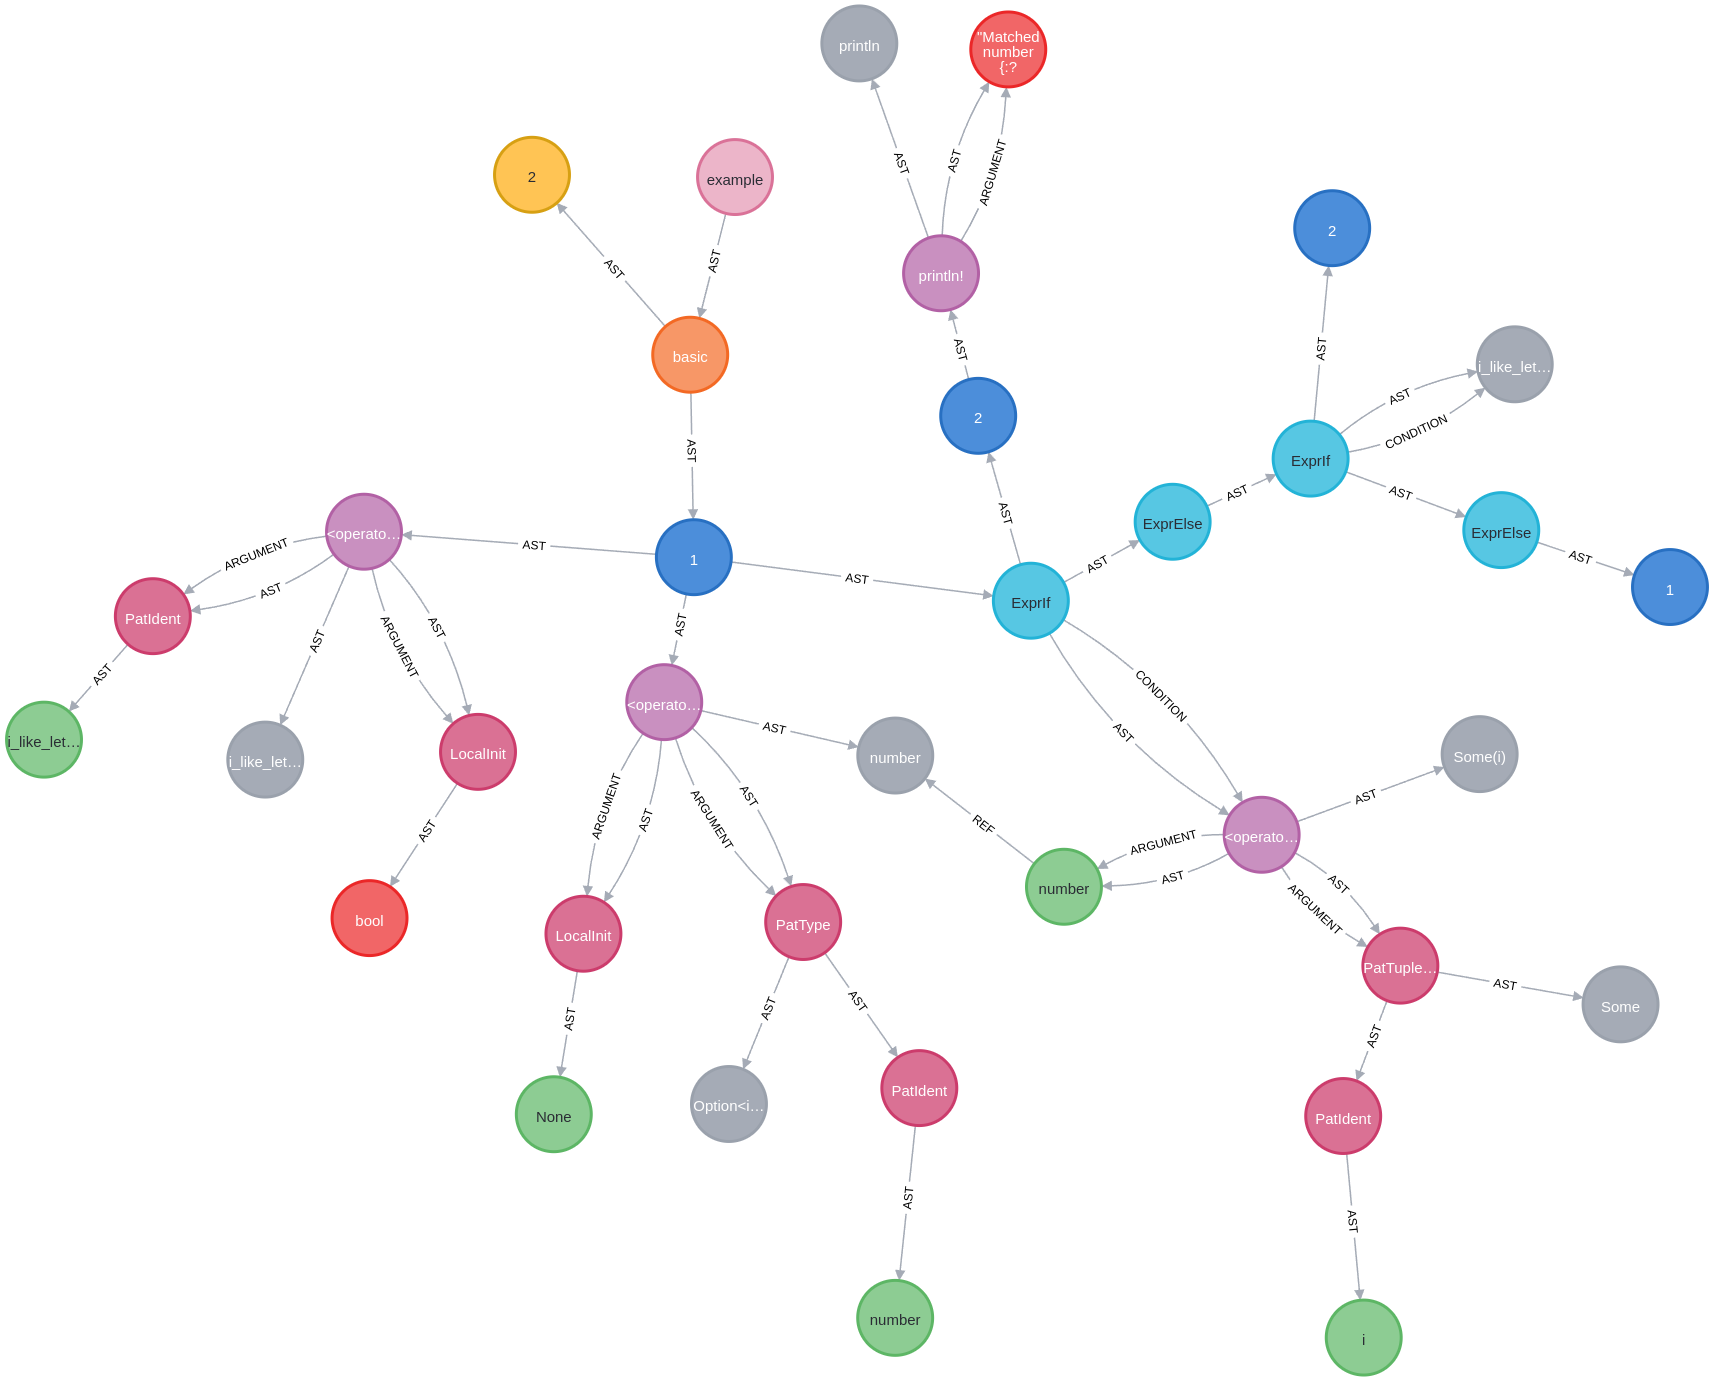
\includegraphics[width=1\columnwidth]{figures/c4/c4_iflet.png}
\centering
\caption{Ví dụ đồ thị CPG cho đoạn mã nguồn if let \ref{code:c4_iflet}}
\label{img:c4_cpg_iflet}
\end{figure}

\subsection{Cú pháp while let}

Tương tự với tính năng if let ở trên, Rust cũng hỗ trợ việc khai báo biến làm điều kiện cho vòng lặp while. Cú pháp của vòng lặp while let như sau:

\begin{minted}[mathescape, breaklines, frame=lines, framesep=2mm, baselinestretch=1.2, fontsize=\footnotesize, linenos]{rust}
while let <pattern> = <expression> {
        <block>
}
\end{minted}

Có thể hiểu là nếu việc khớp giữa \texttt{<pattern>} và \texttt{<expression>} thành công thì sẽ tiếp tục thực hiện vòng lặp, sẽ có 1 biến $i$ mới được khởi tạo đối với mỗi lần lặp.
Các mệnh đề trong khối được thực thi điều kiện của vòng lặp thành công sẽ tham chiếu tới biến $i$ vừa được khai báo thông qua cạnh \texttt{REF} nếu có sử dụng tới.
Không chỉ vậy vế phải của điều kiện \texttt{<expression>} có thể được gán lại liên tục trong quá trình lặp, nếu \texttt{<pattern>} không khớp kết thúc vòng lặp.

\begin{listing}[H]
\begin{minted}[mathescape, breaklines, frame=lines, framesep=2mm, baselinestretch=1.2, fontsize=\footnotesize, linenos]{rust}
let mut optional = Some(0);

while let Some(i) = optional {
    if i > 9 {
        optional = None;
    } else {
        optional = Some(i + 1);
    }
}
\end{minted}
\caption{Ví dụ mã nguồn cho while let}
\label{code:c4_whilelet}
\end{listing}

\begin{figure}[H]
    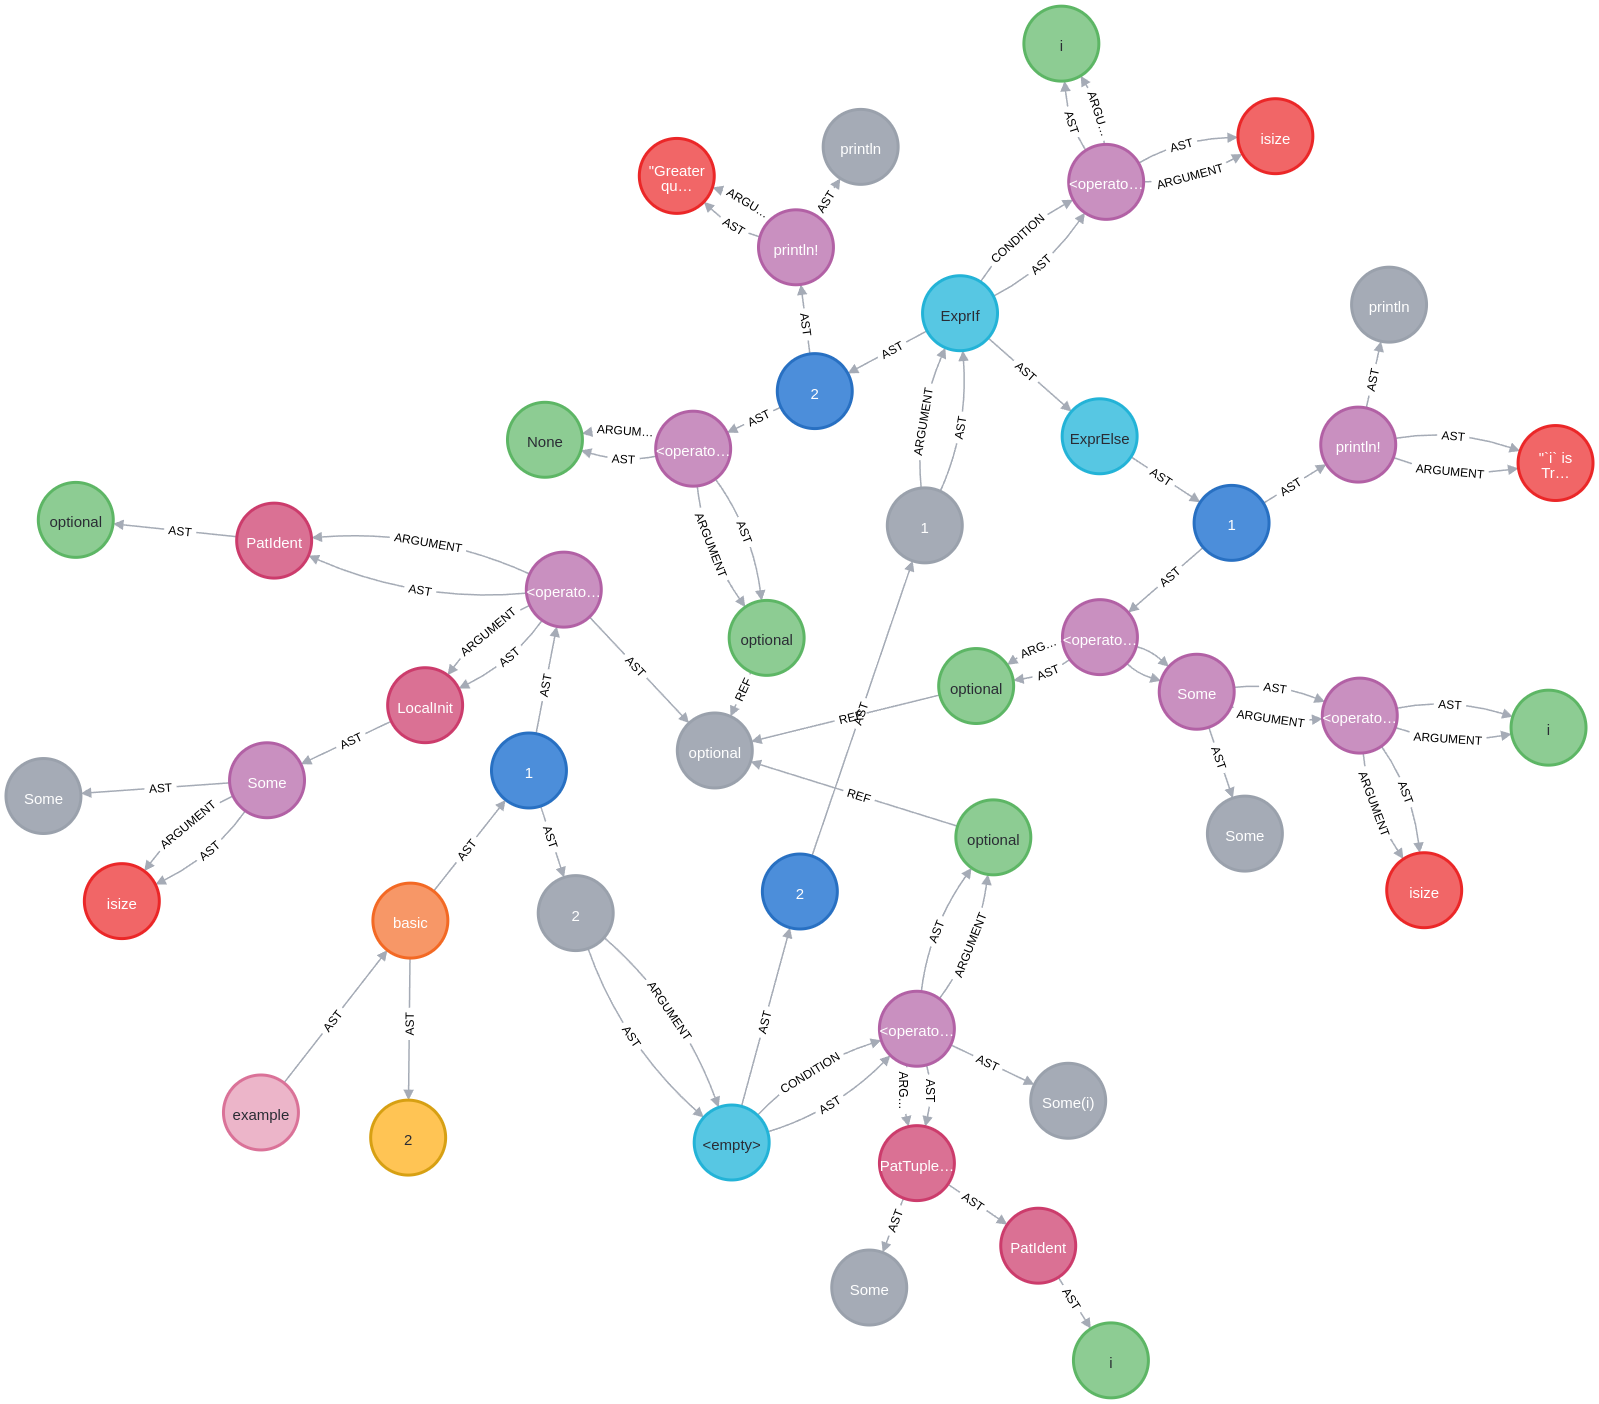
\includegraphics[width=1\columnwidth]{figures/c4/c4_whilelet.png}
    \centering
    \caption{Ví dụ đồ thị CPG cho đoạn mã nguồn while let \ref{code:c4_whilelet}}
    \label{img:c4_cpg_whilelet}
\end{figure}

\subsection{Cú pháp match}

Ngoài việc sử dụng mệnh đề gán biến thành biểu thức điều kiện, tính hướng hàm của Rust còn thể hiện ở tính năng match với sự kết hợp giữa Pattern matching và Algebraic Data Types.
Cấu trúc match không chỉ kiểm tra giá trị mà còn kết hợp với các pattern phức tạp, bao gồm kiểm tra điều kiện, kiểm tra các kiểu dữ liệu khác nhau và so sánh.
Điều này mang lại cho Rust tính linh hoạt cao hơn so với switch trong C/C++ khi chỉ so sánh giá trị nguyên thủy.

Một điểm khác biệt quan trọng giữa match và switch là tính toàn diện của match.
Rust yêu cầu các pattern trong match phải bao quát tất cả các khả năng có thể xảy ra, nếu không trình biên dịch sẽ báo lỗi.
Điều này giúp đảm bảo rằng không có tình huống nào bị bỏ qua, tăng cường độ an toàn của mã nguồn.
Trong khi đó, switch trong C/C++ không yêu cầu bao quát tất cả các trường hợp, và việc bỏ sót một trường hợp có thể dẫn đến lỗi hoặc hành vi không mong muốn.
Thêm vào đó, match trong Rust cho phép trích xuất và xử lý các thành phần của cấu trúc dữ liệu phức tạp ngay trong quá trình đối chiếu pattern.
Ví dụ, Rust có thể match trên \texttt{tuple}, \texttt{enum}, \texttt{struct}, trong khi switch của C/C++ thường chỉ giới hạn trong các giá trị nguyên thủy.

\begin{listing}[H]
\begin{minted}[mathescape, breaklines, frame=lines, framesep=2mm, baselinestretch=1.2, fontsize=\footnotesize, linenos]{rust}
enum Color {
    Red,
    Blue(u32, u32, u32),
    Green { red: u32, green: u32, blue: u32, },
}

fn main() {
    let color = Color::Blue(0, 0, 255);

    match color {
        Color::Red => println!("The color is Red!")
        Color::Blue(r, g, b) => println!("R: {}, G: {}, B: {}!", r, g, b)
        Color::Green {red, green, blue} => println!("R: {}, G: {}, B: {}!", red, green, blue),
    }
}
\end{minted}
\caption{Ví dụ mã nguồn cho match}
\label{code:c4_match}
\end{listing}

\begin{figure}[H]
    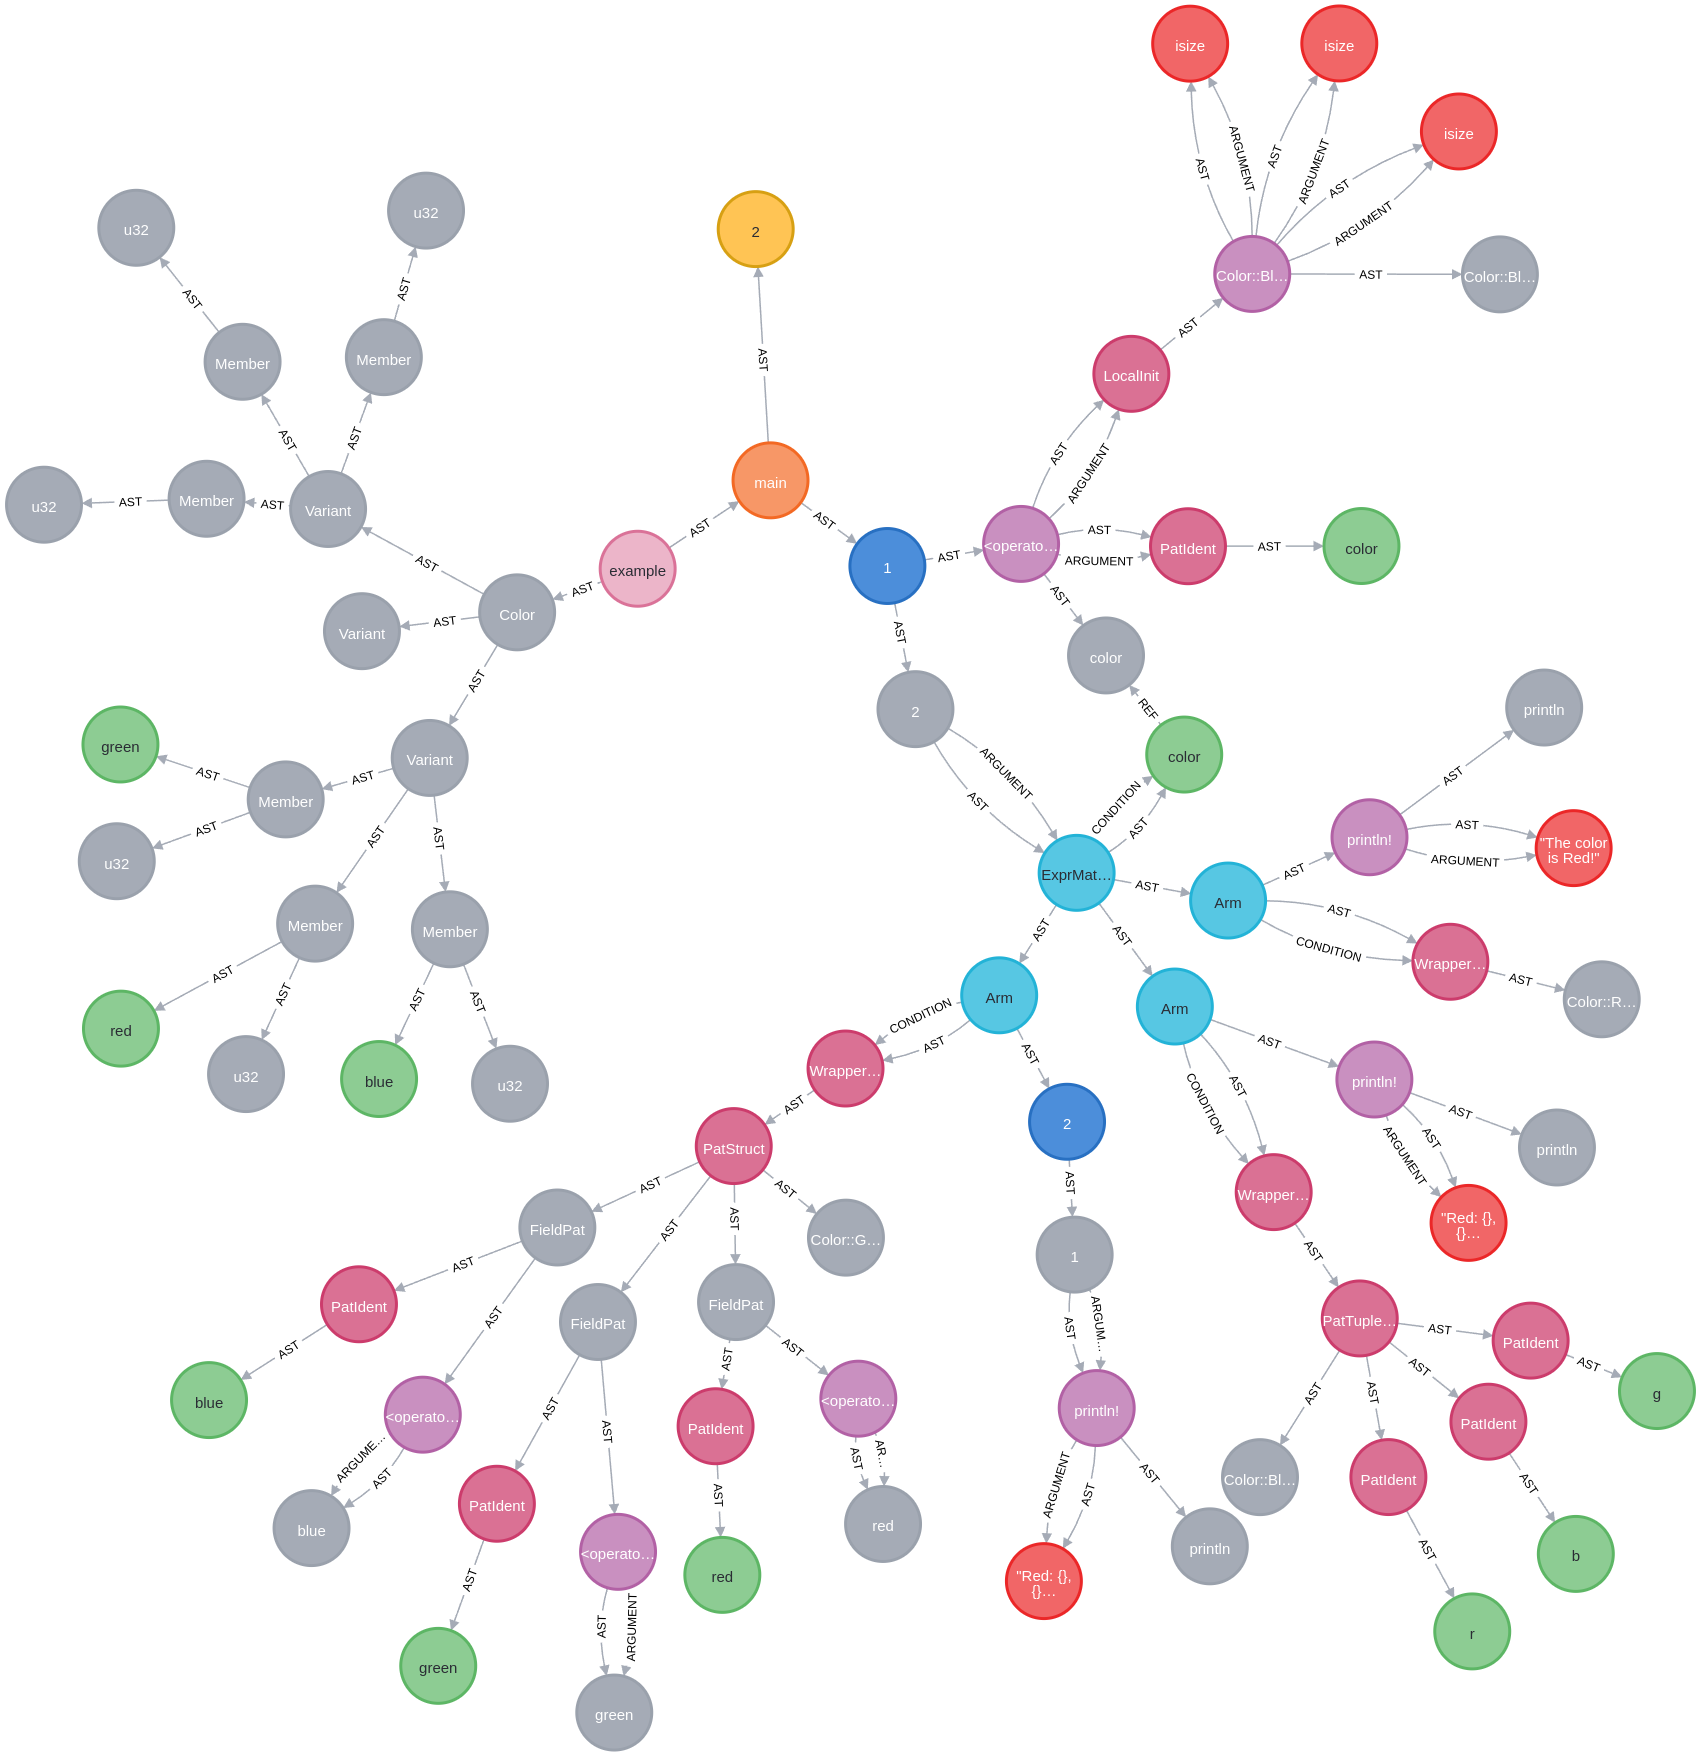
\includegraphics[width=1\columnwidth]{figures/c4/c4_match.png}
    \centering
    \caption{Ví dụ đồ thị CPG cho đoạn mã nguồn match \ref{code:c4_match}}
    \label{img:c4_match}
\end{figure}

\subsection{Cú pháp lifetime}

Lifetime là cơ chế được sử dụng trong Rust để quản lý vòng đời của các biến tham chiếu, đảm bảo rằng các biến tham chiếu không trỏ tới vùng nhớ không còn tồn tại.
Lifetime có vai trò tương tự như kiểu tổng quát, nhưng thay vì định kiểu cho biến thì lifetime sẽ xác định vòng đời cho biến tham chiếu.
Để biểu diễn được tính năng lifetime trên đồ thị CPG, có 3 loại nút mới được thêm vào đặc tả CPG là \texttt{Lifetime}, \texttt{LifetimeParameter}, \texttt{LifetimeArgument}.
Ngoài ra còn có cạnh \texttt{OUT\_LIVE} được bổ sung để chỉ ra quan hệ giữa biến và lifetime, quan hệ giữa các lifetime với nhau.

\texttt{LifetimeParameter} và \texttt{LifetimeArgument} được sử dụng cho các \texttt{struct}, \texttt{enum}, \texttt{trait} để chỉ ra lifetime tổng quát cho các biến tham chiếu.
Loại nút \texttt{Lifetime} sẽ thể hiện vòng đời thực sự của biến tham chiếu.
Các biến tham chiếu sẽ được gán lifetime thông qua việc sử dụng dấu "\texttt{'}" trước tên lifetime, ví dụ như \texttt{'a}.
Nếu các biến cùng đánh dấu lifetime \texttt{'a} thì sẽ có cạnh \texttt{OUT\_LIVE} trỏ từ biến tới nút \texttt{Lifetime} đại diện cho \texttt{'a} tương ứng.
Nếu lifetime \texttt{'a} được giới hạn bởi lifetime \texttt{'b} thì sẽ có cạnh \texttt{OUT\_LIVE} từ nút \texttt{Lifetime} \texttt{'a} tới nút \texttt{Lifetime} \texttt{'b}.

Ownership, borrowing và lifetime là 3 tính năng làm nên cơ chế an toàn bộ nhớ trong Rust.
Do vậy đồ thị CPG phải thể hiện được 3 tính năng trên đồ thị và cung cấp thông tin thông qua các nút, cạnh và thuộc tính phù hợp.
Đặc biệt là tính năng lifetime, vòng đời hợp lệ của các biến được thể hiện qua lifetime do đó việc thể hiện đúng quan hệ giữa lifetime và biến, lifetime với lifetime, biến với biến là rất quan trọng.
Từ đó có thể khai thác thông tin để kiểm tra vòng đời của biến tham chiếu, giúp phát hiện được các lỗi về bộ nhớ gây ra khi đánh dấu lifetime không chính xác.

% Lifetime elision là cơ chế trong Rust giúp tự động suy diễn lifetime cho các biến tham chiếu.
% Có ba luật chính về lifetime elision trong Rust.
% Thứ nhất, mỗi biến tham chiếu đầu vào sẽ được tự động gán lifetime mà không cần phải đánh dấu một cách tường minh.
% Thứ hai, nếu hàm có chỉ có một biến tham chiếu đầu và một biến tham chiếu đầu ra, trình biên dịch sẽ suy luận rằng biến tham chiếu đầu ra có cùng lifetime với biến tham chiếu đầu vào.
% Cuối cùng, nếu hàm có một hoặc nhiều hơn một biến tham chiếu đầu vào và một trong biến đầu vào là biến \texttt{self} (\texttt{self} tương đương với \texttt{this} trong C/C++), trình biên dịch sẽ suy luận rằng biến tham chiếu đầu ra có cùng lifetime với \texttt{self}.
% Ngoài 3 trường hợp trên, Rust yêu cầu phải ghi rõ lifetime cho tất cả các biến tham chiếu để tránh nhầm lẫn và đảm bảo an toàn bộ nhớ.

% \begin{listing}[H]
% \begin{minted}[mathescape, breaklines, frame=lines, framesep=2mm, baselinestretch=1.2, fontsize=\footnotesize, linenos]{rust}
% fn longest<'a>(x: &'a str, y: &'a str) -> &'a str {
%     if x.len() > y.len() {
%         x
%     } else {
%         y
%     }
% }
% \end{minted}
% \caption{Ví dụ mã nguồn cho lifetime cho hàm}
% \label{code:c4_lifetime_1}
% \end{listing}

% \begin{figure}[H]
%     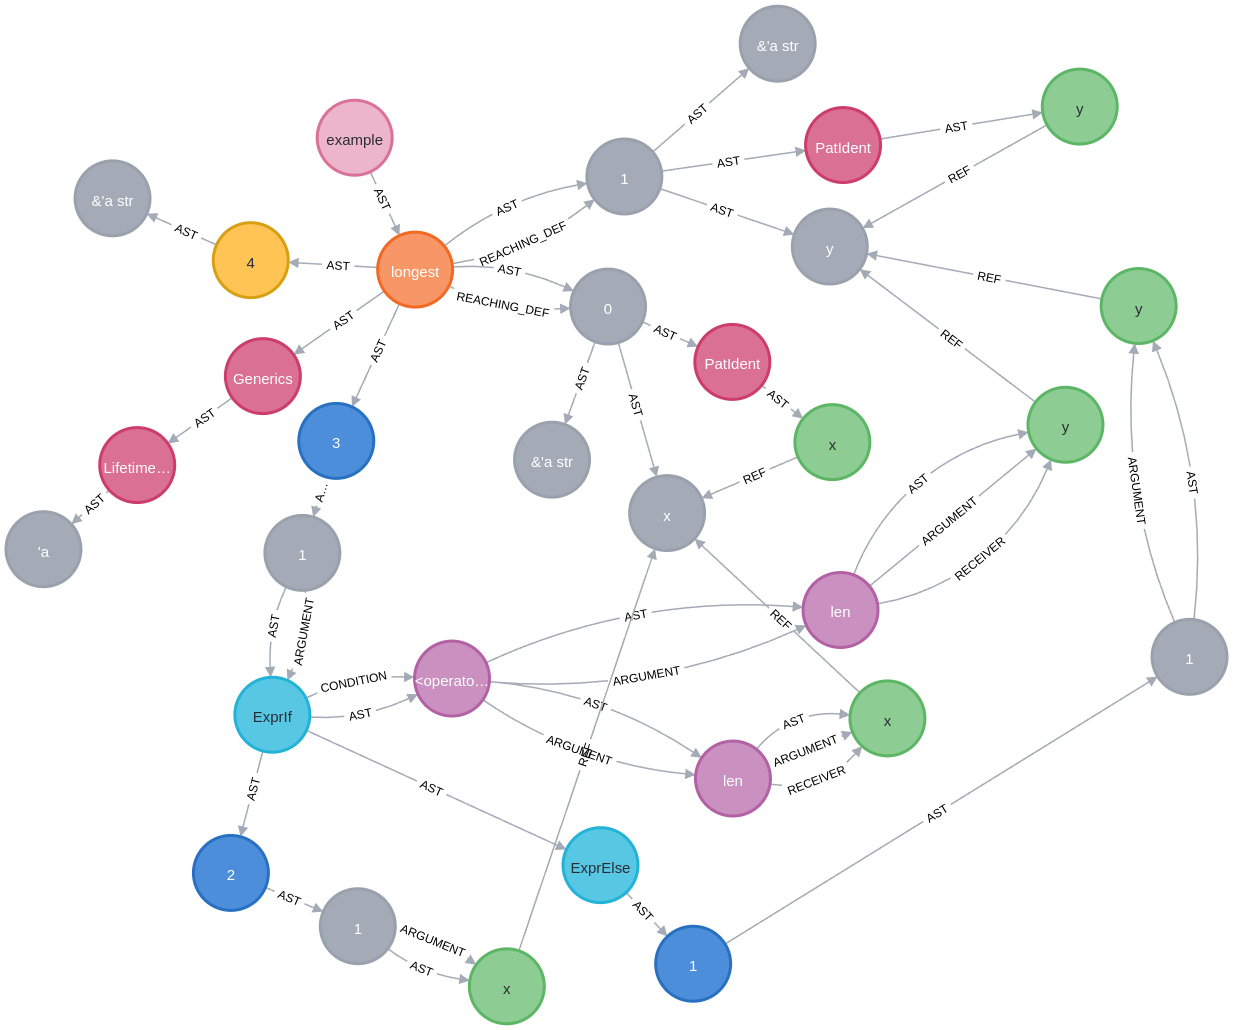
\includegraphics[width=1\columnwidth]{figures/c4/c4_lifetime_1.png}
%     \centering
%     \caption{Ví dụ đồ thị CPG cho đoạn mã nguồn \ref{code:c4_lifetime_1}}
%     \label{img:c4_lifetime_1}
% \end{figure}

\begin{listing}[H]
\begin{minted}[mathescape, breaklines, frame=lines, framesep=2mm, baselinestretch=1.2, fontsize=\footnotesize, linenos]{rust}
fn f<'a, 'b, 'c, 'd: 'c>(x: &'a i32, mut y: &'b i32, z: &'c i32)
where
    'a: 'b,
{
    // ...
}
\end{minted}
\caption{Ví dụ mã nguồn cho giới hạn lifetime}
\label{code:c4_lifetime_2}
\end{listing}

\begin{figure}[H]
    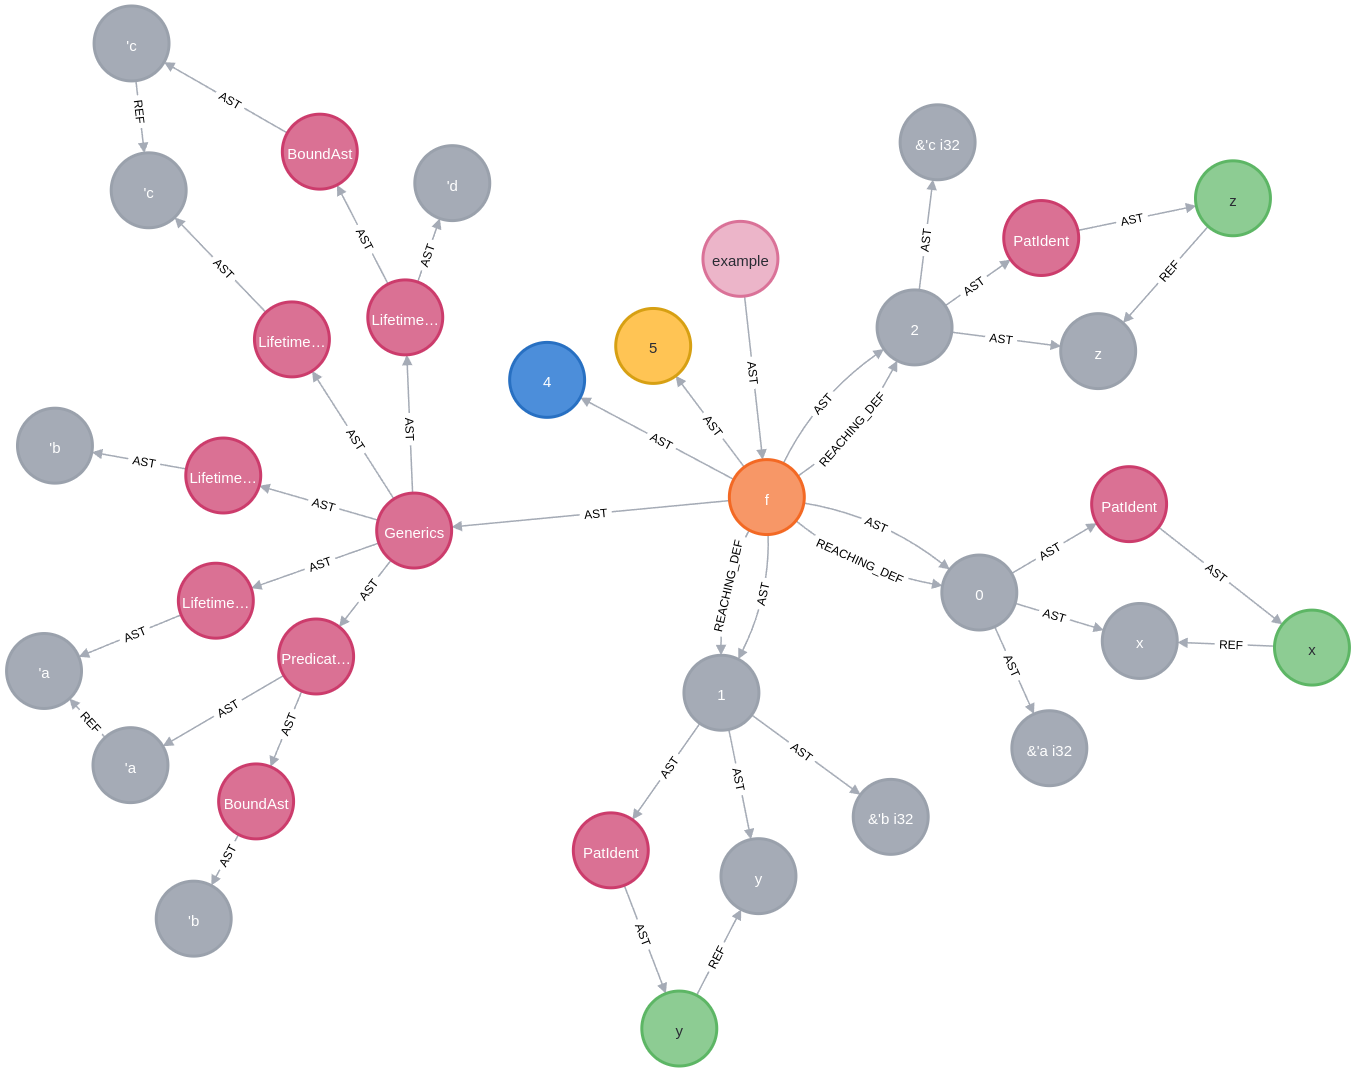
\includegraphics[width=1\columnwidth]{figures/c4/c4_lifetime_2.png}
    \centering
    \caption{Ví dụ đồ thị CPG cho đoạn mã nguồn \ref{code:c4_lifetime_2}}
    \label{img:c4_lifetime_2}
\end{figure}

\section{Hạn chế}

\subsection{Macro}

Trong các ngôn ngữ lập trình như C/C++ và Rust có macro hay còn gọi là metaprogramming. Có thể hiểu macro (metaprogramming) là viết code để sinh ra code, tức là viết code Rust để sinh ra các đoạn code Rust còn lại. Macro trong Rust có 2 loại: declarative macro và procedural macro. Declarative macro giống như macro trong C/C++, còn procedural macro giống như inline function, được xử lý ở bước sinh cây AST. Đối C/C++ có preprossor để xử lý Marco trước khi cho vào compiler, đo đó khi mã nguồn sau khi được tiền xử lý thì đã được xử lý toàn bộ Macro. Tuy nhiên, Rust không giống C/C++, Marco của Rust \cite{rustlangMacrosRust} không được xử lý ở bước sinh cây AST mà sẽ được xử lý sau khi sinh cây AST nhưng trước khi đi vào phase Semantic Ananlysis của trình biên dịch. Như đã để cập ở trên, công cụ hiện tại sử dụng thư viện syn để sinh cây AST cho mã nguồn Rust và syn không hỗ trợ xử lý Macro. Do đó tất cả các mã lệnh nằm bên trong macro sẽ không được xử lý, dẫn đến việc không thể sinh cây AST cho đoạn mã lệnh sử dụng macro. Tất cả các đoạn lệnh nằm trong 1 lời gọi macro hiện tại được xem như 1 chuỗi token. Không chỉ vậy macro trong Rust sử dụng DSL riêng, DSL này gần với ngôn ngữ Rust nhưng có sự mở rộng biến đổi để phù hợp với vai trò macro, do đó không thể sinh cây AST cho macro.

Để xử lý trường hợp trên, ta có thể thêm 1 bước tiền xử lý mã nguồn để giải macro như C/C++. Chúng ta sẽ sử dụng đến thư viện cargo-expand, thư viện này có tác dụng đưa đoạn code Rust macro mà lập trình viên nhìn thấy thành đoạn code Rust mà compiler nhìn thấy. Đoạn code sau khi được mở rộng thì sẽ có được các thông tin bị ẩn đi như prelude mặc định của Rust bao gồm các hàm, symbol được built-in trong ngôn ngữ mà người dùng không phải import thủ công, các macro sẽ được xử lý, bao gồm cả declarative và procedural macro. Đối với declarative macro, thì macro built-in của ngôn ngữ như $println!$, $vec!$ hay kể cả declarative macro do người dùng định nghĩa cũng sẽ được giải.

Tuy nhiên, việc xử lý macro trước khi cho vào cây AST sẽ làm cho mã nguồn bị biến đổi so với mã nguồn gốc, đồng thời tăng kích cỡ và độ lớn của mã nguồn. Việc thêm các thông tin ẩn mà lập trình viên không nhìn thấy có thể gây nhầm lẫn cho người đọc mã nguồn. Điều này cũng đồng nghĩa với việc việc sinh cây AST cho mã nguồn sau khi xử lý macro sẽ phức tạp hơn, việc này sẽ làm tăng thời gian xử lý và độ phức tạp

\subsection{Module}

Cơ chế module trong Rust tương ứng với namespace trong C++, package trong Java. Module chia nhỏ mã nguồn thành các phần nhỏ hơn, tổ chức và quản lý mã nguồn, giúp tái sử dụng mã nguồn, giúp tránh xung đột tên biến, hàm giữa các module khác nhau.
Một module trong Rust có thể là một file riêng biệt hoặc một phần của một file khác. Các module có thể được tổ chức thành một hệ thống phân cấp, với các module con được khai báo bên trong các module cha.
% Có một số file được coi là file đặc biệt trong cấu trúc mã nguồn trong rust.
% Ví dụ như file mod.rs, đây là file module root của thư mục chứa nó, tất cả các module con trong thư mục đó sẽ được import thông qua module root mod.rs.
% Ngoài ra còn có file main.rs, lib.rs để đánh dấu điểm đầu vào của chương trình và xác định xem dự án là 1 thư viện hay 1 ứng dụng.
Rust còn cung cấp cơ chế workspace, cho phép quản lý nhiều dự án nhỏ trong cùng 1 dự án lớn, mỗi dự án là 1 thư mục con trong thư mục workspace.
Để kiểm soát khả năng truy cập, Rust sử dụng cơ chế visibility. Mặc định các thành phần trong module là private, để làm cho chúng có thể truy cập được từ các module khác, ta sử dụng từ khóa pub.
Cơ chế path resolution dùng để định danh 1 thành phần cấu trúc từ module khác ta mà ta có thể import. Path resolution có thể là đường dẫn tuyệt đối hoặc tương đối. Ví dụ dùng từ khóa $self$ để chỉ tới module hiện tại, dùng từ khóa $super$ để chỉ tới module cha của module hiện tại, $crate$ để chỉ tới module root của dự án.
Hệ thống module phức tạp của Rust làm tăng đáng kể độ khó việc xử lý quan hệ giữa các module trong cây AST và phân tích ngữ cảnh.
Việc xử lý các khái niệm như module con, module gốc, visibility, import và path resolution đòi hỏi một cơ chế phân tích tinh vi, do vậy hiện tại công cụ chưa xử lý module

% \subsection{Path}

% \begin{itemize}
%     \item Path có thể là Absolute Path hoặc Relative Path tùy vào bối cảnh module hiện tại, path có thể chỉ tới đối tượng trong cùng 1 module hoặc khác module
%     \item Path trong Rust là đường dẫn đến 1 đối tượng nào đó được định nghĩa trong mã nguồn như struct, trait, static, const, function
%     \item Cây AST sử dụng thư viện $syn$, $syn$ có thể lấy được path của 1 đối tượng nhưng không biết được đối đượng đang trỏ tới là static, const, hay function. Do đó đang không phân biệt được đâu là path của static, const, hay function
% \end{itemize}

% \subsection{Type Argument match Type Parameter}


% \section{Phân tích mã nguồn có lỗ hổng bảo mật}

Theo báo cáo đến năm 2023, tổng cộng có 17 thể loại bug được báo cáo về RUSTSEC Database \cite{zheng2023closer}.
Trong đó, lỗi về an toàn bộ nhớ và đa luồng chiếm tới gần hai phần ba tổng số loại lỗi.
Mặc dù Rust có các cơ chế để khắc phục những lỗi này, nhưng dường như trong những dự án thực tế phức tạp, vẫn tồn tại một số lỗi nhất định, đặc biệt khi sử dụng tính năng \texttt{unsafe} (mã không an toàn) của Rust.
Để minh họa cho việc áp dụng đồ thị CPG vào thực tế, khóa luận sẽ trình bày ứng dụng của đồ thị CPG trên 4 lỗi trong RUSTSEC Database thuộc các thể loại lỗi phổ biến nhất.

\subsection{RUSTSEC-2021-0086}

RUSTSEC-2021-0086 là lỗi về khởi tạo bộ nhớ không an toàn.
Lỗi này xảy ra khi sử dụng hàm \texttt{Vec::with\_capacity} để khởi tạo một vectơ với dung lượng được định sẵn, sau đó sử dụng hàm \texttt{set\_len} để điều chỉnh độ dài của vectơ.
Tuy nhiên hàm \texttt{set\_len}, một hàm được coi là \texttt{unsafe}, nó không khởi tạo giá trị cho các phần tử của vectơ mà chỉ sửa lại độ dài của vectơ, dẫn đến việc các phần tử có giá trị là không xác định.
Để sửa lỗi, ta có thể sử dụng macro \texttt{vec!} để khởi tạo vectơ với độ dài và dung lượng là $N$, giá trị mặc định của mỗi phần tử là $0$.

\begin{listing}[H]
\begin{minted}[mathescape, breaklines, frame=lines, framesep=2mm, baselinestretch=1.2, fontsize=\footnotesize, linenos]{rust}
const N: usize = 255;

// Before fix
let mut buf: Vec<u8> = Vec::with_capacity(N);
unsafe { buf.set_len(N) };

// After fix
let mut buf: Vec<u8> = vec![0; N];
\end{minted}
\caption{Ví dụ đoạn mã nguồn cho RUSTSEC-2021-0086}
\label{code:c4_RUSTSEC-2021-0086}
\end{listing}

\begin{figure}[H]
    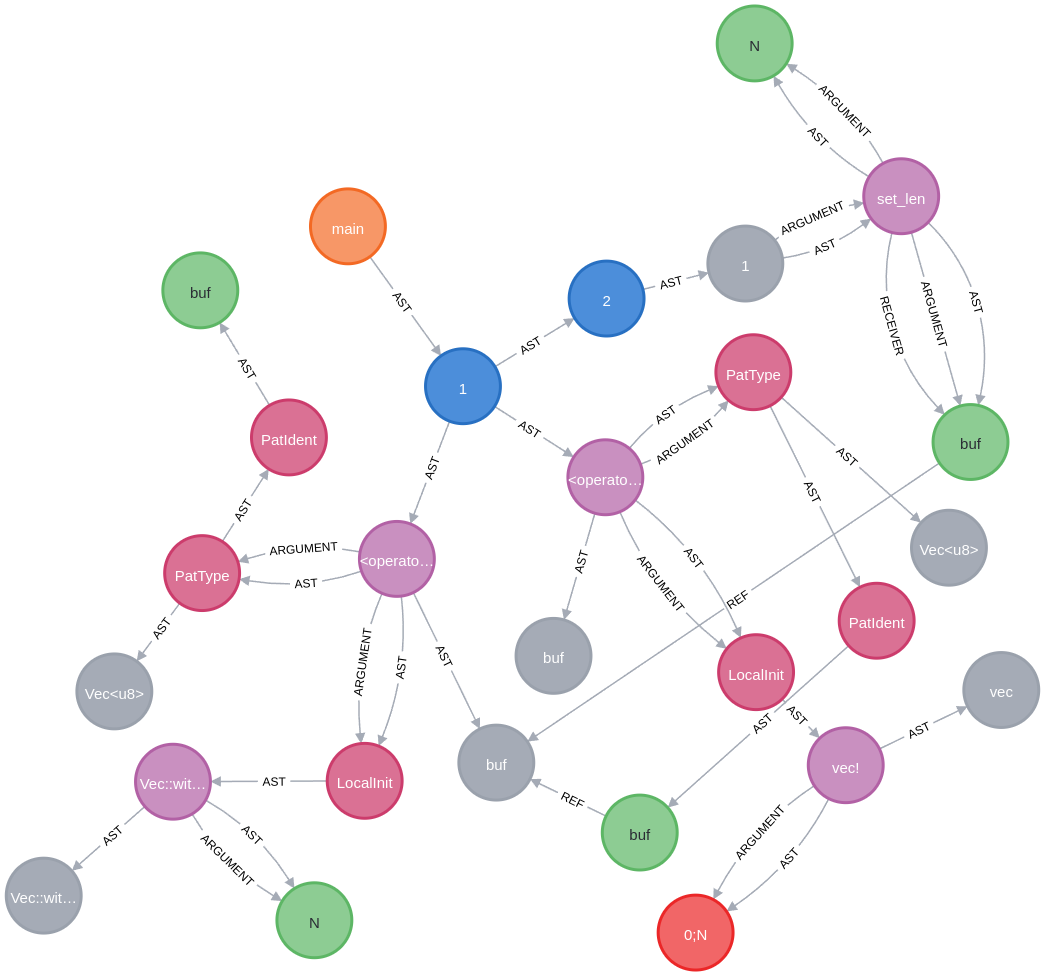
\includegraphics[width=1\columnwidth]{figures/c4/c4_RUSTSEC-2021-0086}
    \centering
    \caption{Minh họa đồ thị CPG cho đoạn mã nguồn RUSTSEC-2021-0086 \ref{code:c4_RUSTSEC-2021-0086}}
    \label{img:c4_RUSTSEC-2021-0086}
\end{figure}

\subsection{RUSTSEC-2022-0028}

Lỗi RUSTSEC-2022-0028 xảy ra khi sử dụng hàm \texttt{external} mà không xác dịnh đúng ràng buộc lifetime cho kiểu tổng quát \texttt{T}.
Trong bối cảnh này, \texttt{ArrayBuffer} là hàm được dùng để giao tiếp giữa Rust và Javascript thông qua Web Assembly Binding \cite{ githubGitHubRustwasmwasmbindgen}.
Điều này cho phép tạo ra một \texttt{ArrayBuffer} từ các kiểu dữ liệu có thể bị giải phóng trong khi chúng vẫn được tham chiếu bởi \texttt{ArrayBuffer} trong Javascript.
Để sửa lỗi, cần thêm ràng buộc \texttt{T: 'static} để đảm bảo rằng dữ liệu được tham chiếu sẽ không bị giải phóng trong suốt thời gian tồn tại của \texttt{ArrayBuffer}.

\begin{listing}[H]
\begin{minted}[mathescape, breaklines, frame=lines, framesep=2mm, baselinestretch=1.2, fontsize=\footnotesize, linenos]{rust}
// Before fix
pub fn external<'a, C, T>(cx: &mut C, data: T) -> Handle<'a, Self>
where
    C: Context<'a>,
    T: AsMut<[u8]> + Send,
{
    // ...
}

// After fix
pub fn external<'a, C, T>(cx: &mut C, data: T) -> Handle<'a, Self>
where
    C: Context<'a>,
    T: AsMut<[u8]> + Send + 'static,
{
    // ...
}
\end{minted}
\caption{Ví dụ đoạn mã nguồn cho RUSTSEC-2022-0028}
\label{code:c4_RUSTSEC-2022-0028}
\end{listing}

\begin{figure}[H]
    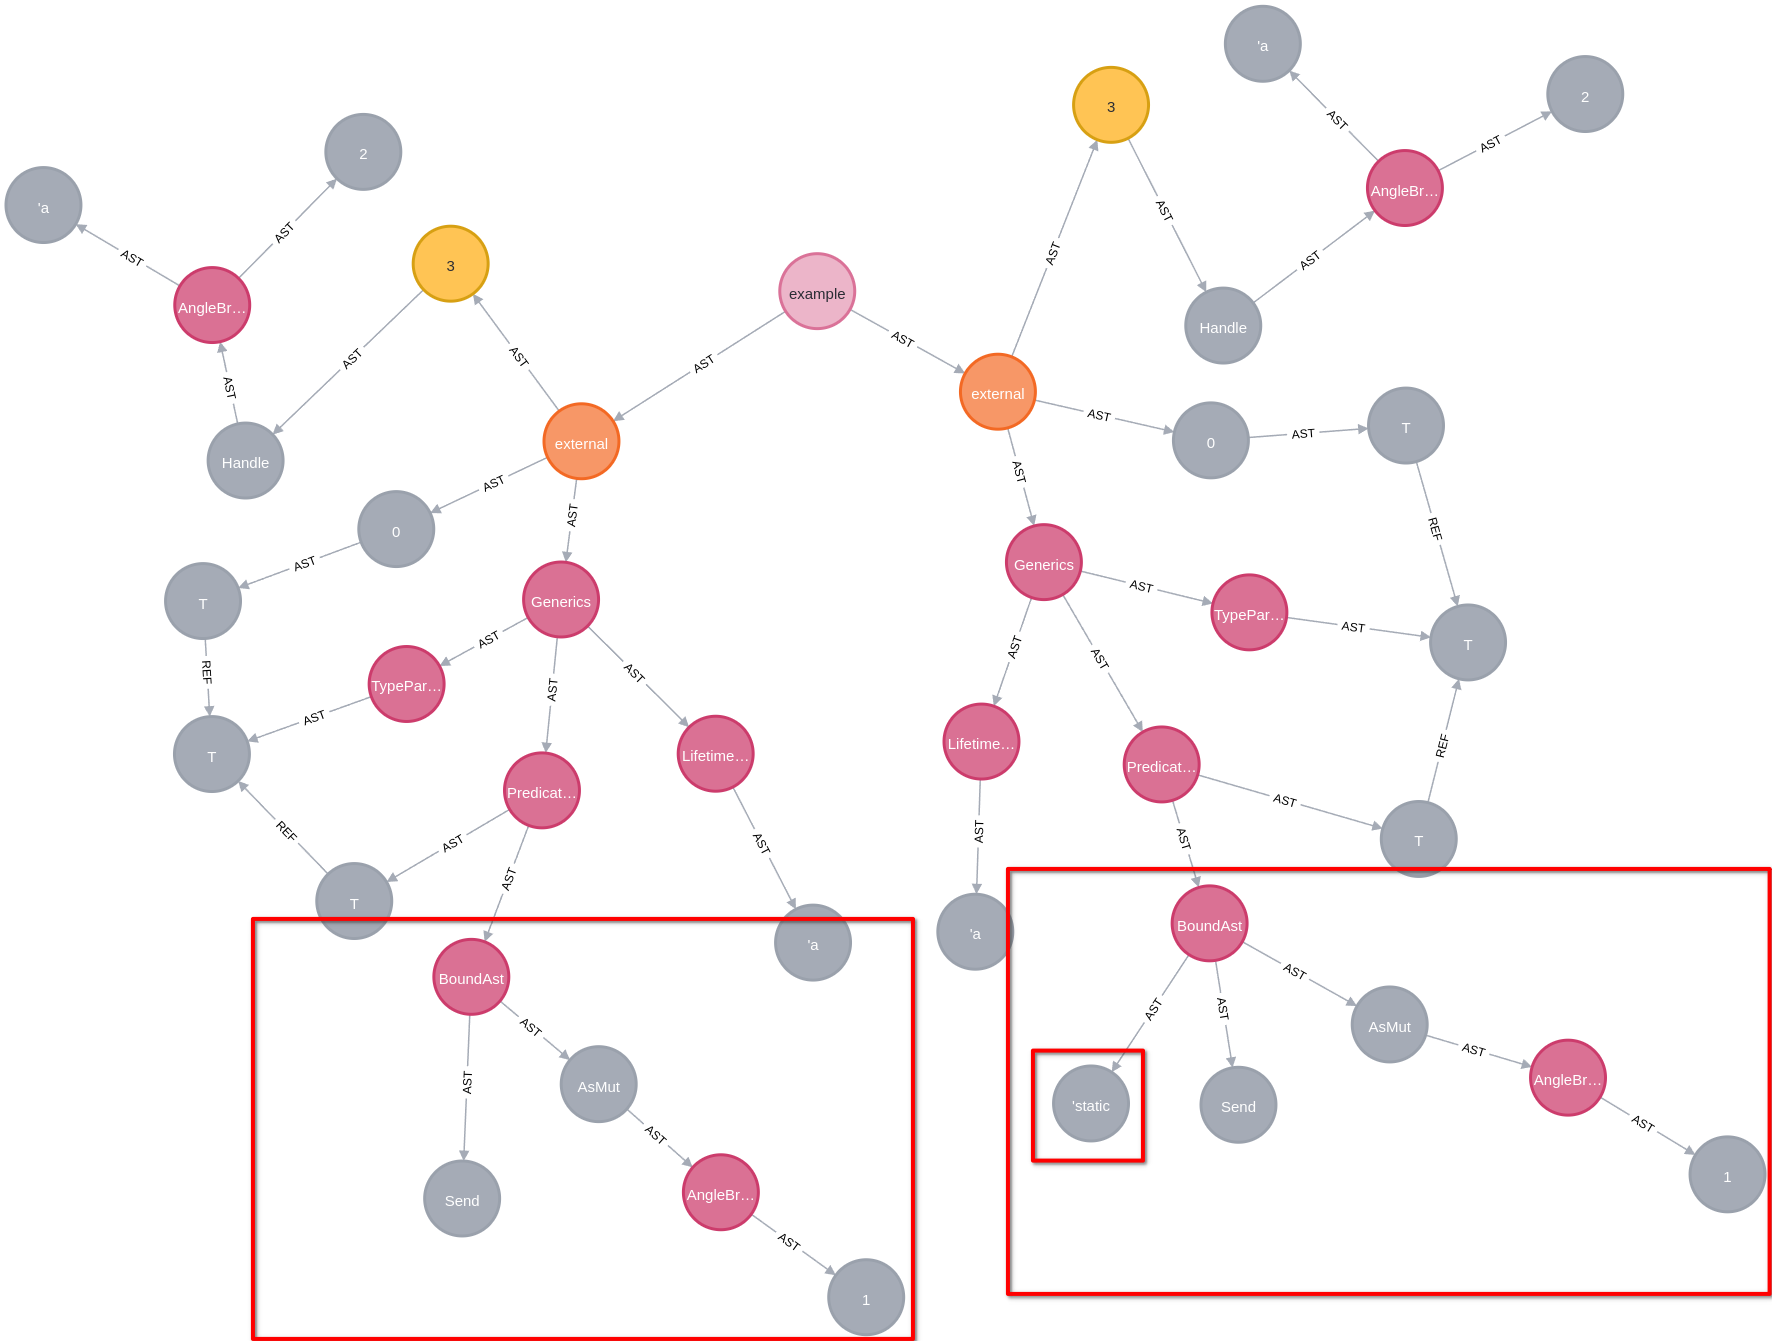
\includegraphics[width=1\columnwidth]{figures/c4/c4_RUSTSEC-2022-0028.png}
    \centering
    \caption{Minh họa đồ thị CPG cho đoạn mã nguồn RUSTSEC-2022-0028 \ref{code:c4_RUSTSEC-2022-0028}}
    \label{img:c4_RUSTSEC-2022-0028}
\end{figure}

\subsection{RUSTSEC-2020-0044}

RUSTSEC-2020-0044 là lỗi liên quan đến việc không triển khai thuộc tính \texttt{Send} cho kiểu dữ liệu con của kiểu \texttt{Atom}.
Trong bối cảnh này, \texttt{Atom} đóng vai trò như một "hộp" cho kiểu dữ liệu \texttt{P} bên trong, giúp quản lý việc sử dụng bộ nhớ an toàn hơn.
Tuy nhiên chỉ mình \texttt{Atom} được cài đặt thuộc tính \texttt{Send} và \texttt{Sync}, không đảm bảo rằng kiểu dữ liệu con \texttt{P} cũng phải cài đặt thuộc tính \texttt{Send}.
Điều này có nghĩa việc truy cập đến \texttt{Atom} có thể an toàn nhưng khi truy cập vào dữ liệu kiểu \texttt{P} bên trong thì không an toàn, có thể dẫn đến các vấn đề như sử dụng bộ nhớ sau khi đã giải phóng hoặc tương tranh dữ liệu cho kiểu dữ liệu \texttt{P} bên trong.
Để sửa lỗi này, cần đảm bảo rằng kiểu \texttt{P} cũng phải được đánh dấu thuộc tính \texttt{Send}.
Điều này có nghĩa là nếu kiểu cha muốn được gửi qua các luồng một cách an toàn bằng thuộc tính \texttt{Send} thì kiểu con \texttt{P} cũng phải có khả năng này, tương tự với trait \texttt{Sync}.

\begin{listing}[H]
\begin{minted}[mathescape, breaklines, frame=lines, framesep=2mm, baselinestretch=1.2, fontsize=\footnotesize, linenos]{rust}
// Before fix
unsafe impl<P> Send for Atom<P> where P: IntoRawPtr + FromRawPtr {}
unsafe impl<P> Sync for Atom<P> where P: IntoRawPtr + FromRawPtr {}

// After fix
unsafe impl<P> Send for Atom<P> where P: IntoRawPtr + FromRawPtr + Send {}
unsafe impl<P> Sync for Atom<P> where P: IntoRawPtr + FromRawPtr + Send {}
\end{minted}
\caption{Ví dụ đoạn mã nguồn cho RUSTSEC-2020-0044}
\label{code:c4_RUSTSEC-2020-0044}
\end{listing}

\begin{figure}[H]
    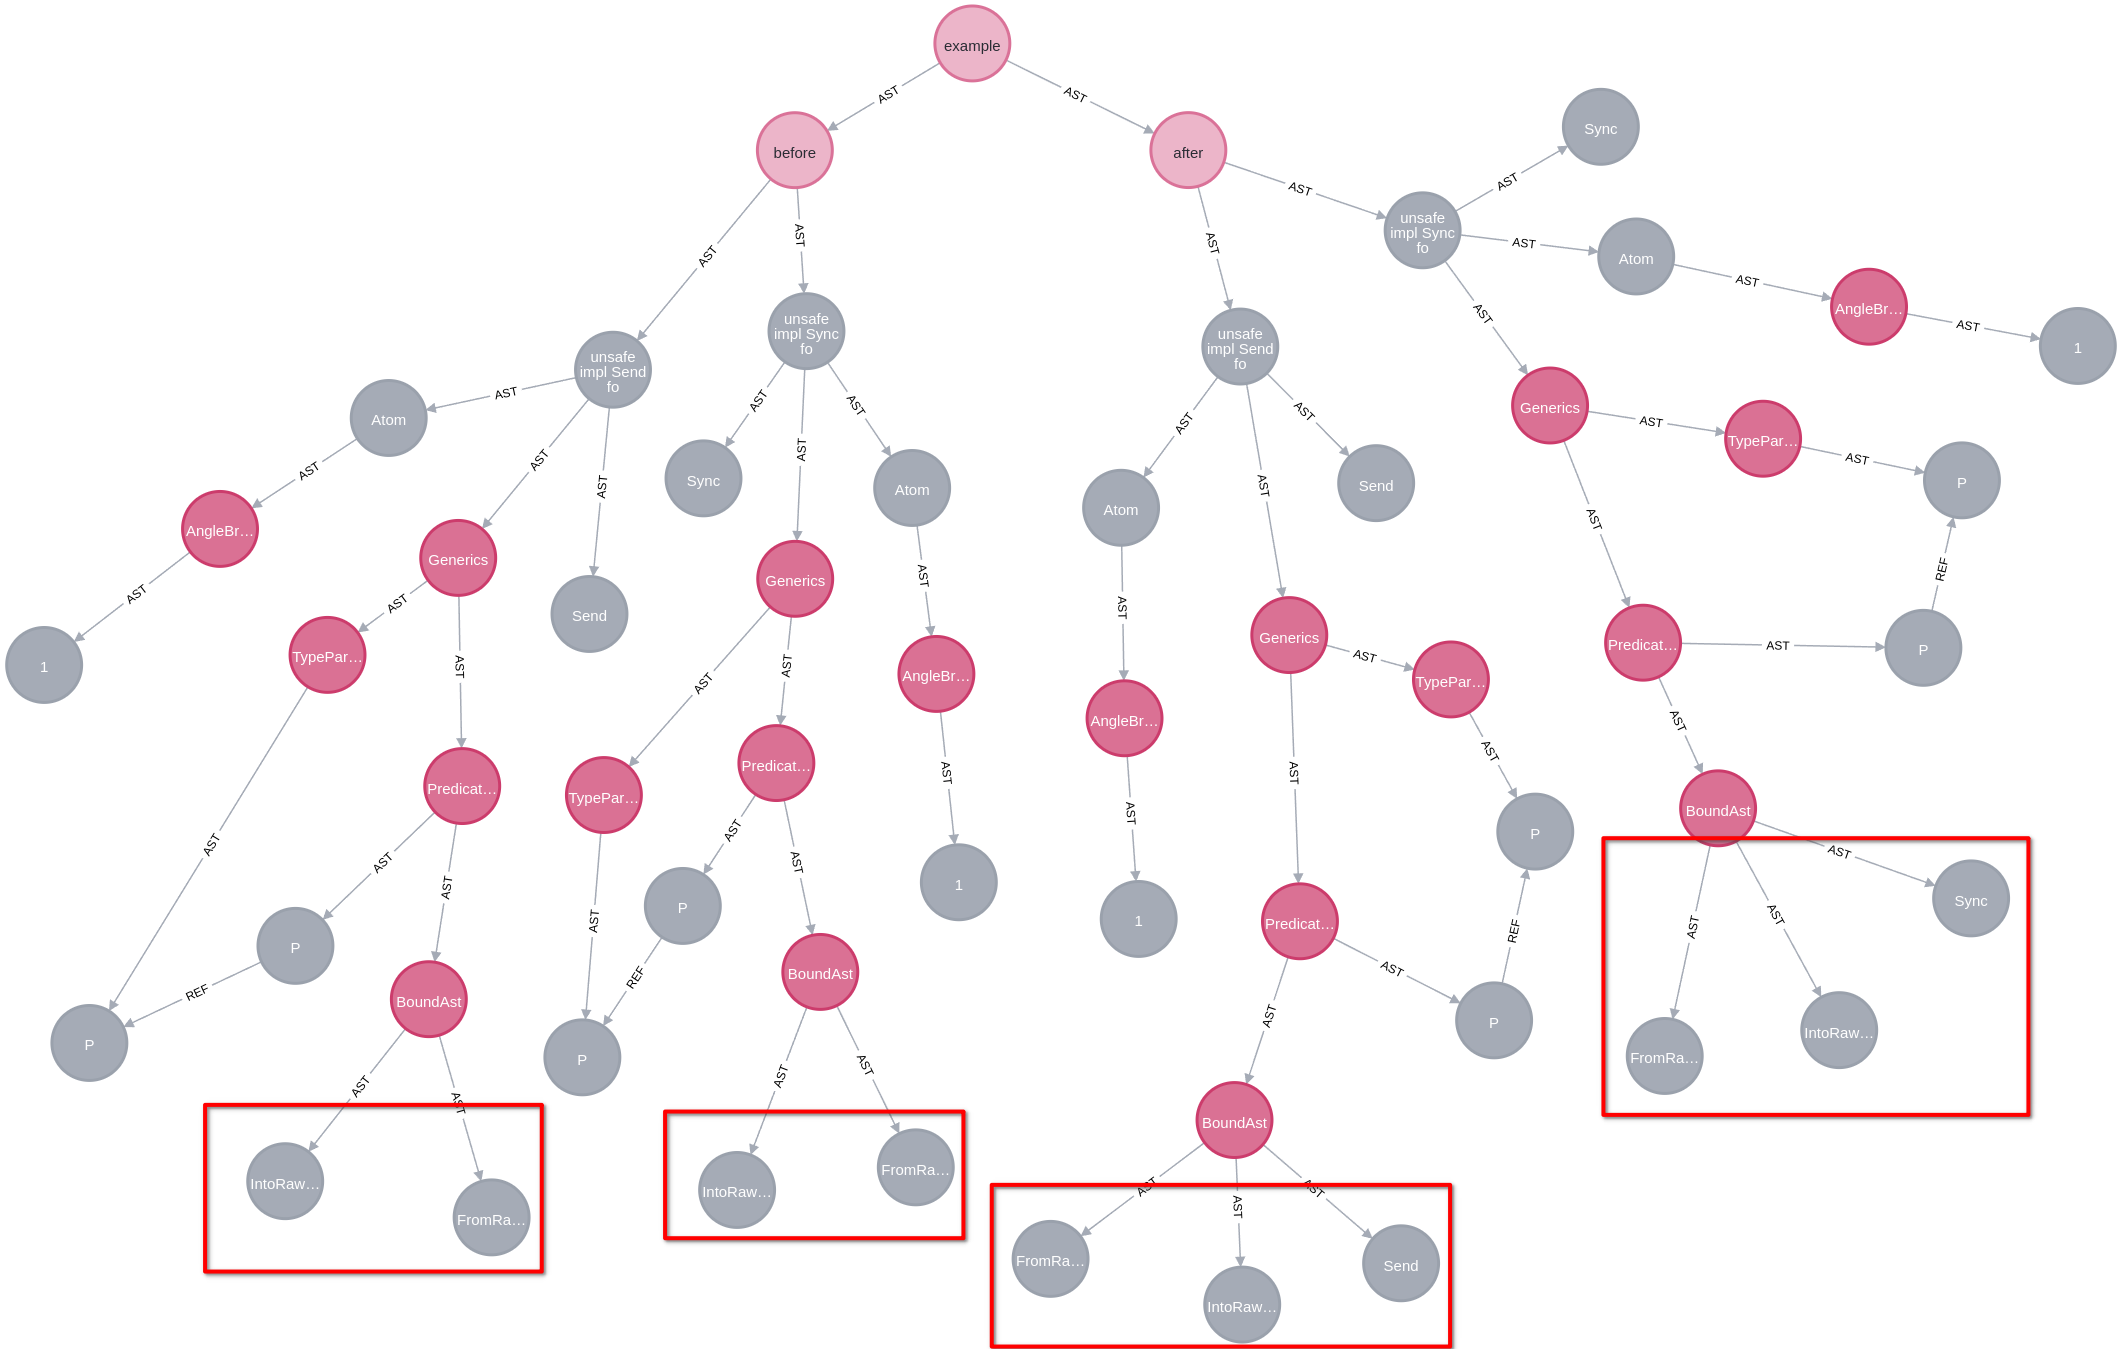
\includegraphics[width=1\columnwidth]{figures/c4/c4_RUSTSEC-2020-0044.png}
    \centering
    \caption{Minh họa đồ thị CPG cho đoạn mã nguồn RUSTSEC-2020-0044 \ref{code:c4_RUSTSEC-2020-0044}}
    \label{img:c4_RUSTSEC-2020-0044}
\end{figure}

Kiểu cha muốn đảm bảo an toàn về đa luồng thì kiểu con cũng phải đảm bảo an toàn về đa luồng.
Đây là một mẫu có thể được xây dựng và áp dụng cho nhiều đoạn mã khác.
Các truy vấn hoặc phân tích dựa trên mẫu này có thể được áp dụng trên đồ thị CPG để phát hiện các lỗi tương tự.

\subsection{RUSTSEC-2021-0130}

RUSTSEC-2021-0130 là lỗi về sử dụng bộ nhớ sau khi đã giải phóng.
Trong bối cảnh này, \texttt{Iter} là một \texttt{struct} được sử dụng để duyệt qua các phần tử trong một danh sách liên kết.
Tuy nhiên, khi \texttt{Iter} được trả về từ hàm \texttt{iter} thì nó sẽ trỏ tới \texttt{self.head} mà \texttt{self.head} có thể bị giải phóng trước khi \texttt{Iter} được sử dụng, dẫn đến việc sử dụng bộ nhớ sau khi đã giải phóng.
Nguyên nhân là do quan hệ lifetime giữa biến \texttt{self} và giá trị trả về kiểu \texttt{Iter} không đồng bộ.
Biến \texttt{self} được chỉ định lifetime là \texttt{'\_}, tức là để trình biên dịch tự gán một giá trị lifetime mặc định, trong khi đó kiểu trả về \texttt{Iter} được chỉ định lifetime là \texttt{'a}.
Trong trường hợp này \texttt{'\_} và \texttt{'a} không có liên hệ với nhau do đó lifetime của \texttt{Iter} có thể lớn hơn lifetime của \texttt{self}, dẫn đến việc truy cập đến \texttt{self.head} sau khi \texttt{self} đã bị giải phóng.
Để sửa lỗi, cần sử dụng cùng chung một lifetime cho \texttt{self} và \texttt{Iter} thông qua việc sử dụng quy tắc 3 của lifetime ellision.
Nếu không chỉ định lifetime một cách tường minh, ba quy tắc lifetime ellision sẽ được trình biên dịch sử dụng để tự động xác định lifetime của các biến dựa trên cấu trúc của hàm, bao gồm:

\begin{enumerate}
    \item Mỗi tham số kiểu tham chiếu của hàm mặc định có một lifetime riêng.
    \item Khi hàm có một tham số duy nhất kiểu tham chiếu, và kiểu trả về cũng là kiểu tham chiếu thì lifetime của kiểu trả về sẽ là lifetime của tham số duy nhất đó.
    \item Nếu hàm có nhiều tham số kiểu tham chiếu nhưng có một tham số là \texttt{self} (\texttt{self} tương đương với \texttt{this} trong C++ và Java), thì lifetime của \texttt{self} sẽ được gán cho kiểu tham số trả về.
\end{enumerate}

Trong trường hợp này sửa lỗi bằng cách không chỉ định lifetime cho \texttt{self} mà để trình biên dịch tự xác định, lifetime của \texttt{Iter} sẽ để là \texttt{'\_}, tức là tự động suy diễn và áp dụng quy tắc 3 của lifetime ellision thì lifetime của \texttt{Iter} sẽ được gán bằng lifetime của \texttt{self}.
Từ đó lifetime của \texttt{Iter} sẽ không lớn hơn lifetime của \texttt{self} và việc truy cập đến \texttt{self.head} sau khi \texttt{self} đã bị giải phóng sẽ không xảy ra.

\begin{listing}[H]
\begin{minted}[mathescape, breaklines, frame=lines, framesep=2mm, baselinestretch=1.2, fontsize=\footnotesize, linenos]{rust}
// Before fix
pub fn iter<'a>(&'_ self) -> Iter<'a, K, V> {
    Iter { ptr: unsafe { (*self.head).next }, }
}

// After fix
pub fn iter(&self) -> Iter<'_, K, V> {
    Iter { ptr: unsafe { (*self.head).next }, }
}
\end{minted}
\caption{Ví dụ đoạn mã nguồn cho RUSTSEC-2021-0130}
\label{code:c4_RUSTSEC-2021-0130}
\end{listing}

\begin{figure}[H]
    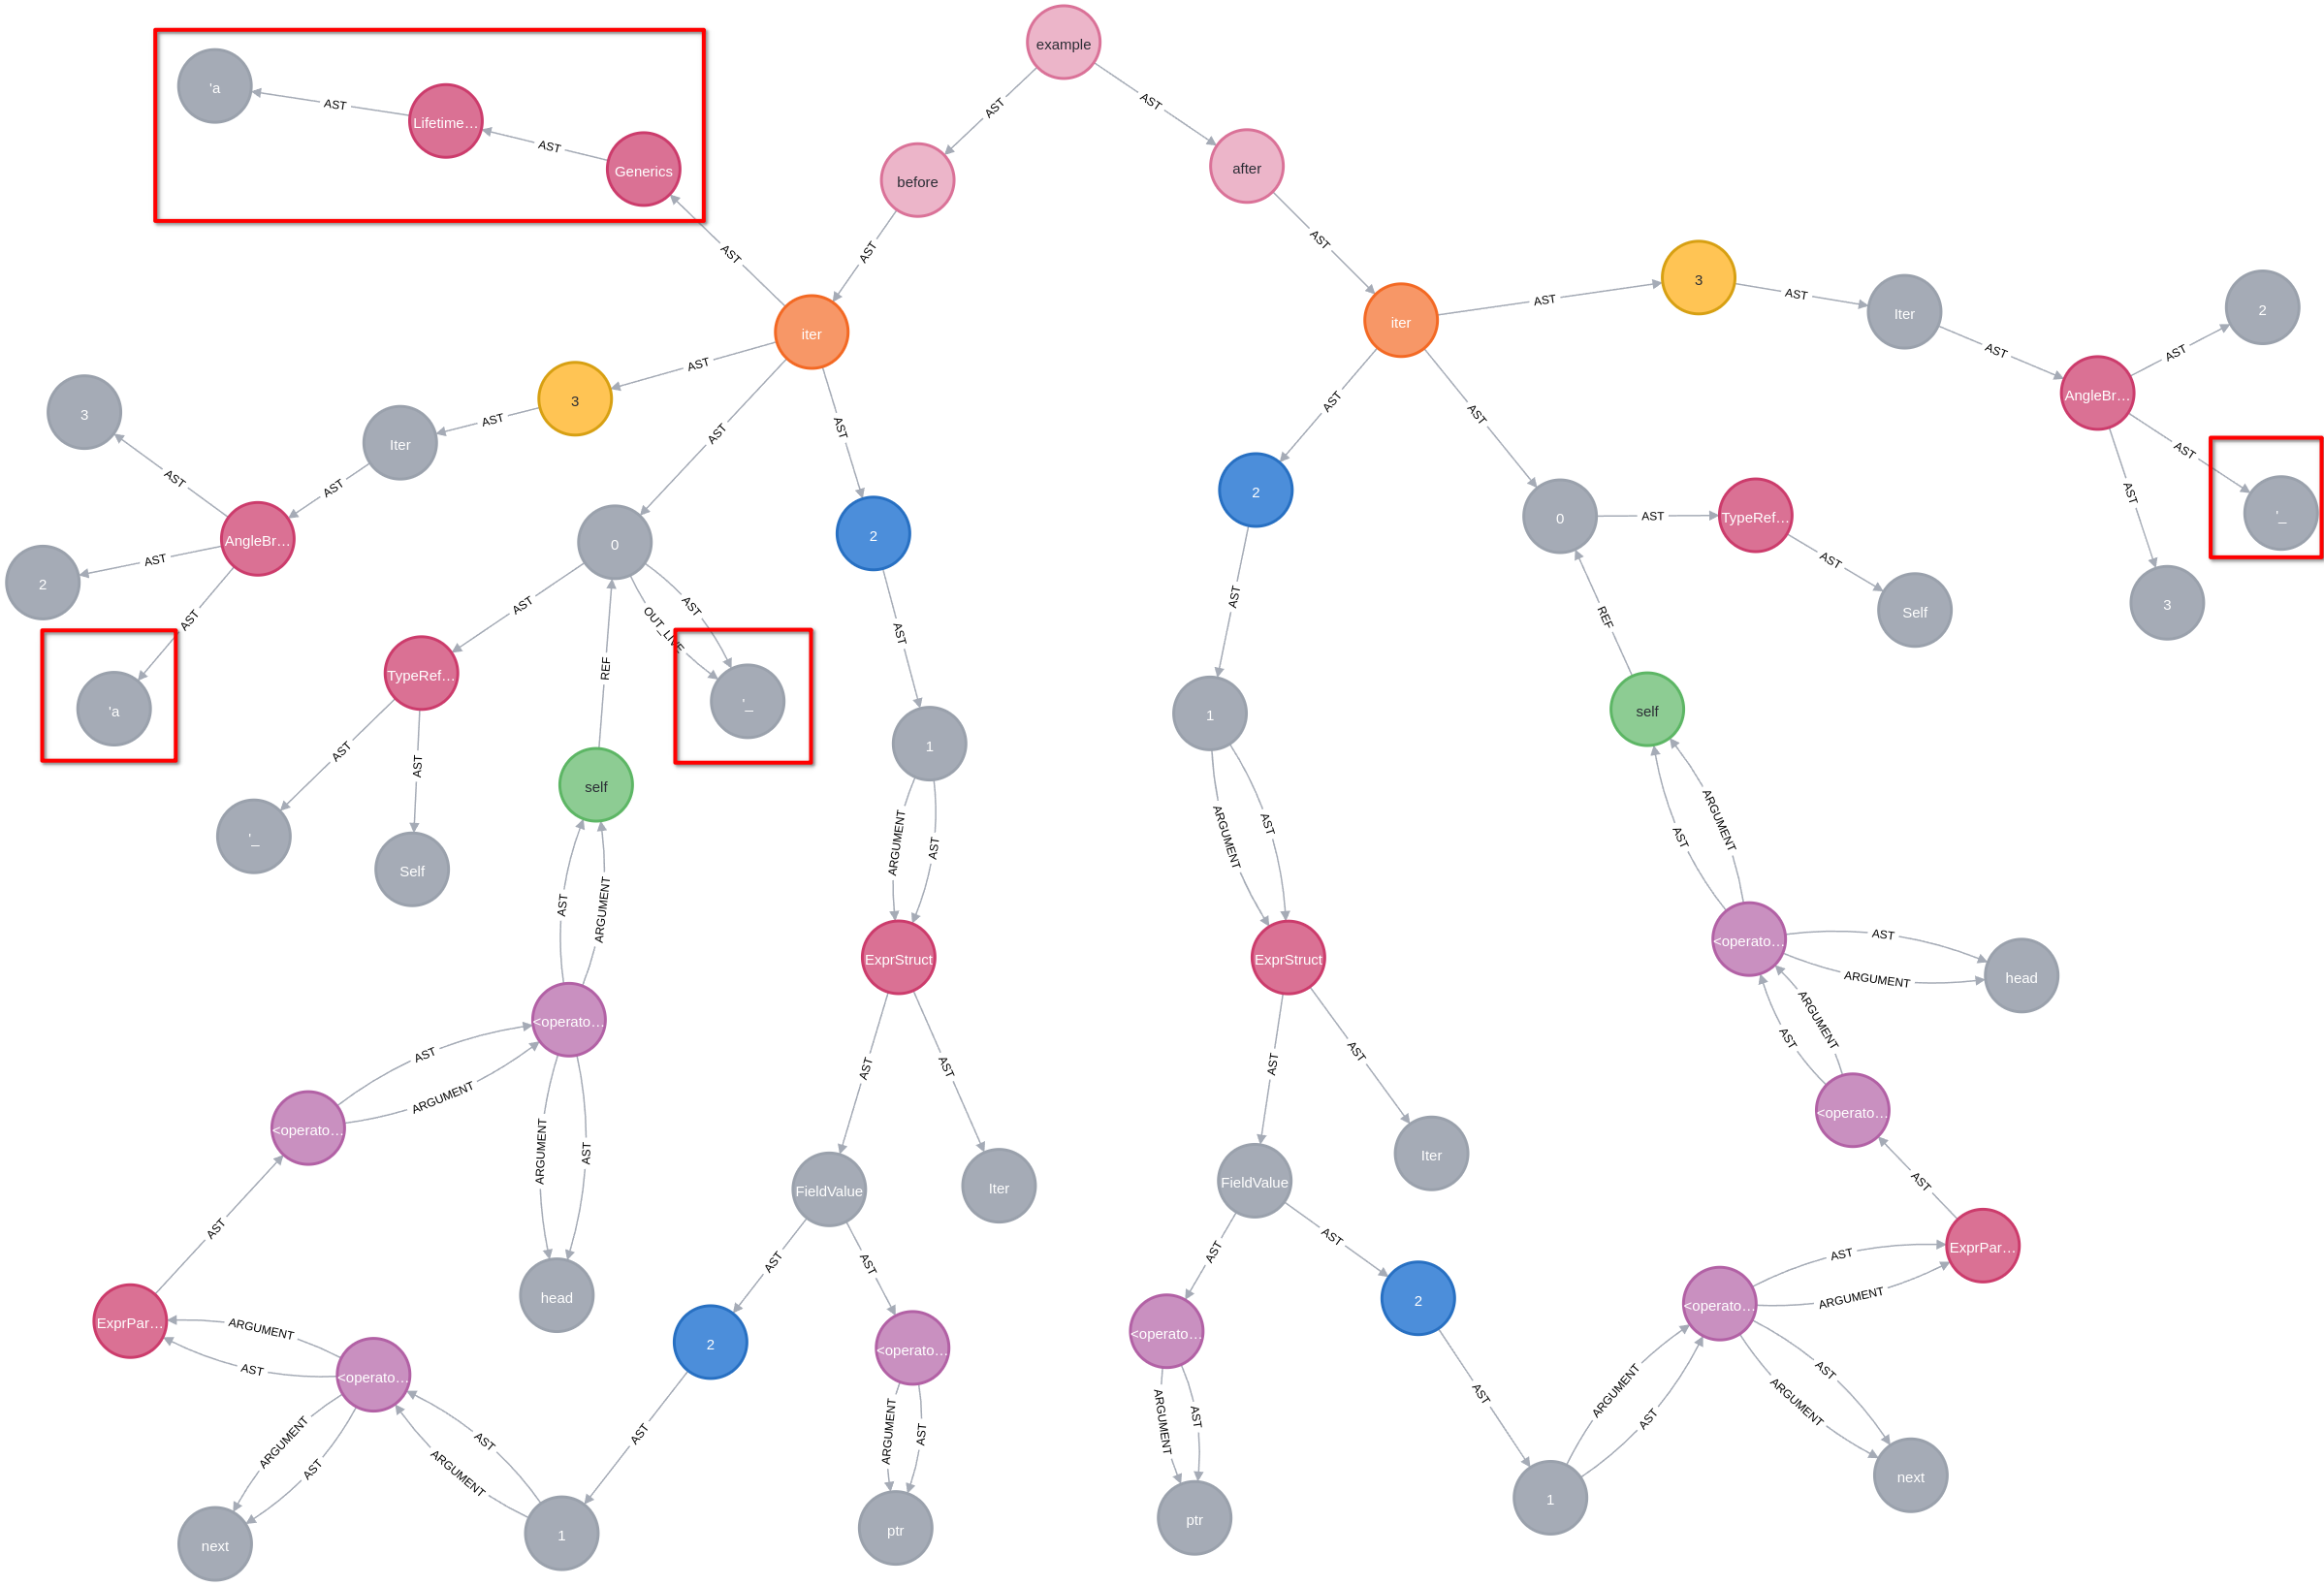
\includegraphics[width=1\columnwidth]{figures/c4/c4_RUSTSEC-2021-0130.png}
    \centering
    \caption{Minh họa đồ thị CPG cho đoạn mã nguồn RUSTSEC-2021-0130 \ref{code:c4_RUSTSEC-2021-0130}}
    \label{img:c4_RUSTSEC-2021-0130}
\end{figure}

Đánh dấu lifetime một cách tường minh cần được thực hiện cẩn thận để tránh được các lỗi liên quan đến bộ nhớ.
Việc đánh dấu lifetime không chính xác có thể đánh lừa trình biên dịch và dẫn đến việc sử dụng bộ nhớ sau khi đã giải phóng.
Lifetime của kiểu trả về phải đảm bảo không lớn hơn lifetime của tham số truyền vào nếu kiểu trả về có truy cập đến bộ nhớ của tham số truyền vào.
Có thể áp dụng các quy tắc lifetime ellision để suy diễn việc xác định lifetime giữa tham số và tham số, giữa tham số và kiểu trả về.
Các luật có thể được đề ra để phát hiện sự không đồng bộ về lifetime giữa các biến, từ đó giúp phát hiện lỗi về bộ nhớ trên đồ thị CPG.

% \section{Ứng dụng bài toán học máy trên đồ thị CPG}

% Mục tiêu thực nghiệm là Bài toán phân loại
% Dữ liệu
% Độ đo đánh giá
% Baseline
% Kết quả thực nghiệm

Để chứng minh tiềm năng của đồ thị CPG dành cho ngôn ngữ Rust, khóa luận xây dựng một thực nghiệm sử dụng kỹ thuật học máy để phát hiện lỗ hổng bảo mật trong mã nguồn Rust dựa trên đồ thị CPG.
Bài toán đặt ra là phân loại tệp mã nguồn Rust có lỗ hổng bảo mật và không có lỗ hổng bảo mật.
Thực nghiệm sẽ tiến hành so sánh độ hiệu quả giữa mô hình học máy sử dụng đồ thị CPG và mô hình học máy học sử dụng mã nguồn Rust truyền thống.
Mô hình học máy chỉ sử dụng dữ liệu mã nguồn Rust, tạm gọi là Baseline, sẽ sử dụng phương pháp Word2Vec \cite{church2017word2vec} để biểu diễn mã nguồn và Logistic Regression \cite{lavalley2008logistic} để phân loại.
Đối với bài toán học máy để phát hiện lỗ hổng bảo mật trên đồ thị CPG, trước đây đã có phương pháp Devign, một phương pháp kinh điển cho lớp bài toán này \cite{zhou2019devign}.
Devign đã sử dụng đồ thị CPG cho ngôn ngữ C/C++, do đó hoàn toàn có thể áp dụng phương pháp Devign với đồ thị CPG cho ngôn ngữ Rust trong khóa luận này.

Bộ dữ liệu được sử dụng bao gồm 788 tệp mã nguồn, trong đó 381 tệp có lỗ hổng bảo mật và 407 tệp không có lỗ hổng bảo mật.
Đối với 381 tệp có lỗ hổng bảo mật, các tệp này được trích xuất từ bộ dữ liệu trong nghiên cứu của David Lo và cộng sự \cite{zheng2023closer}.
Còn 407 tệp không có lỗ bảo mật được thu thập từ 100 dự án mã nguồn mở của Rust nhiều sao nhất trên Github \cite{githubGithubRankingTop100RustmdMaster} và xác nhận thủ công.
Tập dữ liệu được chia thành 3 phần, 80\% dữ liệu được sử dụng cho quá trình huấn luyện, 10\% dữ liệu được sử dụng cho kiểm chứng, 10\% dữ liệu được sử dụng cho kiểm thử.
Để đánh giá, mỗi phương pháp được chạy 10 lần đối với tập dữ liệu như trên.
Kết quả của các chỉ số là giá trị trung bình của 10 lần chạy.
Kết quả thực nghiệm được thể hiện bằng bảng phía dưới.

Với bài toán phân loại, thang đo đánh giá hiệu suất của phương pháp sẽ bao gồm các chỉ số Accuracy, Precision, Recall và F1-score.
% ROC AUC, Precision-Recall AUC, MCC, Error Rate
Accuracy biểu thị tỷ lệ phần trăm các dự đoán đúng trên tổng số các dự đoán, thể hiện độ chính xác tổng thể của mô hình, nhưng có thể không phản ánh đúng với dữ liệu mất cân bằng.
Precision đo độ chính xác trong việc phân loại đúng một lớp cụ thể, hữu ích khi cần giảm thiểu dự đoán dương tính sai.
Recall, hay độ nhạy, đánh giá khả năng phát hiện đầy đủ các mẫu thuộc một lớp, đặc biệt quan trọng trong việc giảm thiểu bỏ sót các trường hợp dương tính.
F1-score là chỉ số thể hiện sự cân bằng giữa Precision và Recall, giúp đánh giá hiệu suất chung của cả hai chỉ số quan trọng này.

\begin{table}[H]
    \centering
    \caption{Bảng so sánh phương pháp Baseline và phương pháp Devign (Rust).}
    \label{table:c4_ml}
    \begin{tabular}{l @{\hskip 3cm} c @{\hskip 3cm} c}
        \hline
         & Baseline & \textbf{Devign (Rust)} \\
        \hline
        Accuracy & 0.73 & \textbf{0.76} \\
        Precision & 0.73 & \textbf{0.76} \\
        Recall & 0.70 & \textbf{0.99} \\
        F1-score & 0.72 & \textbf{0.86} \\
        % ROC AUC & 0.81 & \textbf{0.47} \\
        % Precision-Recall AUC & 0.74 & \textbf{0.78} \\
        % MCC & 0.46 & \textbf{0.01} \\
        % Error Rate & 0.27 & \textbf{0.23} \\
        \hline
    \end{tabular}
\end{table}

Trong Bảng \ref{table:c4_ml}, phương pháp Devign đã cho kết quả tốt hơn so với phương pháp Baseline với hầu hết các chỉ số.
Ta thấy được Accuracy hơn 0.03, Precision hơn 0.03, Recall hơn 0.29, F1-Score hơn 0.16.
% , Precision-Recall AUC hơn 0.04 và Error Rate thấp hơn 0.04.
% Tuy nhiên, ROC AUC và MCC của phương pháp Devign lại thấp hơn so với phương pháp Baseline.
Điều này chứng tỏ rằng đồ thị CPG cho ngôn ngữ Rust có tiềm năng áp dụng cho bài toán phát hiện lỗ hổng bảo mật kết hợp bằng kỹ thuật học máy.
Mã nguồn và bộ dữ liệu sử dụng trong thực nghiệm được lưu trữ lần lượt tại địa chỉ \href{https://github.com/congnghiahieu/devign}{devign}, \href{https://github.com/congnghiahieu/rust-ecosystem}{rust-ecosystem}.

Độ chính xác của phương pháp Devign cho ngôn ngữ Rust mới chỉ đạt được ở mức 0.76 bởi một vài nguyên do.
Thứ nhất là kích cỡ của bộ dữ liệu cho ngôn ngữ Rust.
Hiện tại các mã nguồn có lỗi được xác nhận đều lấy từ RUSTSEC Database.
Rust là ngôn ngữ mới phát triển gần đây, hệ sinh thái chưa lớn mạnh nên số lượng mã nguồn có lỗi được báo cáo không nhiều.
Thứ hai là đồ thị CPG của Rust vẫn chưa đầy đủ hoàn toàn.
Tồn tại các tính năng của Rust như marco, module chưa thể phân tích ra cây AST hay lấy được các lớp thông tin cần thiết.
Các hạn chế này sẽ được trình bày chi tiết ở phần \ref{sec:limit}.
% Các lớp thông tin về CFG, PDG vẫn chưa được hoàn thiện, hay các lớp thông tin khác có giá trị khai thác được sinh ra từ Joern cũng chưa được cung cấp.
Thứ ba là giới hạn trong cài đặt của phương pháp Devign.
Hiện tại, phiên bản cài đặt của Devign là mô phỏng lại từ bài báo gốc.
Devign mới chỉ có thể sử dụng lớp thông tin về AST và CFG mà không có PDG, do vậy không thể khai thác được hết toàn bộ thông tin từ đồ thị CPG.
% chưa kể các lớp thông tin khác của Joern CPG.
Nếu có thể khắc phục được các hạn chế kể trên, phương pháp Devign có thể đạt được kết quả tốt hơn nữa.

Dù tồn tại những hạn chế, kết quả thực nghiệm vẫn cho thấy tiềm năng khai thác to lớn của đồ thị CPG cho ngôn ngữ Rust.
Đồ thị CPG có thể được sử dụng cho các lớp bài toán cần đến phân tích mã nguồn như phát hiện lỗ hổng bảo mật, phân loại mã nguồn hay các ứng dụng khác trong tương lai.
Ngoài ra, việc cải thiện và hoàn thiện đồ thị CPG cho ngôn ngữ Rust sẽ mở ra nhiều hướng nghiên cứu và ứng dụng mới.
Điều này không chỉ giúp nâng cao hiệu quả của các phương pháp hiện tại mà còn thúc đẩy sự phát triển của hệ sinh thái ngôn ngữ Rust.

\newpage\cleardoublepage
\chapter*{Kết luận}
\addcontentsline{toc}{chapter}{Kết luận}

Phân tích mã nguồn là một bước quan trọng trong quá trình phát triển phần mềm. Quá trình này sẽ giúp phát hiện các lỗi, lỗ hổng bảo mật và vấn đề tiềm ẩn tồn tại trong mã nguồn, đồng thời nó giúp lập trình viên phát hiện các lỗi logic, tối ưu mã nguồn và đảm bảo các quy tắc và tiêu chuẩn khi lập trình. Điều này giúp sớm phát hiện các lỗi nghiêm trọng, đảm bảo tính ổn định, dễ quản lý và dễ bảo trì cho mã nguồn về sau.

Hiện nay trên thế giới có khoảng 20 ngôn ngữ lập trình thông dụng và đi kèm với đó là hàng trăm công cụ phân tích mã nguồn khác nhau. Khóa luận này đã xây dựng thành công một công cụ phân tích mã nguồn dành cho ngôn ngữ lập trình Rust. Khác so với các công cụ phân tích mã nguồn hiện có, công cụ chọn phân tích mã nguồn thành đồ thị thuộc tính mã nguồn thay vì chỉ phân tích thành cây cú pháp trừu tượng bởi lẽ dạng đồ thị này là tổng hợp của cây cú pháp trừu tượng, đồ thị dòng điều khiển và đồ thị thuộc tính mã nguồn. Nó không chỉ cung cấp thông tin về cú pháp trong mã nguồn mà còn cung cấp cả thông tin về luồng điều khiển và phụ thuộc dữ liệu trong chương trình. Đồng thời công cụ cũng được phát triển dựa trên công cụ có sẵn là Joern nên nó kế thừa được những tiện ích mạnh mẽ sẽ giúp cho quá trình khai thác mã nguồn dựa trên đồ thị thuộc tính mã nguồn trở nên dễ dàng và chuyên sâu hơn. Qua quá trình thực nghiệm công cụ với bộ dự án mã nguồn Rust phổ biến, công cụ đã đáp ứng được những mục tiêu đề ra của khóa luận khi đã xử lý được thông tin về kiểu dữ liệu, phân tích được phần lớn các cú pháp mã nguồn Rust và đưa ra kết quả chi tiết và đầy đủ hơn so với công cụ Joern. Tuy nhiên, công cụ vẫn chưa xử lý được toàn bộ các cú pháp mã nguồn mà Rust cung cấp, việc phân tích còn tốn nhiều thời gian đặc biệt là với các dự án có sử dụng nhiều thư viện bên ngoài do việc xử lý kiểu dữ liệu đòi hỏi phải phân tích cả những thư viện đi kèm.

Trong tương lai, công cụ phân tích mã nguồn Rust sẽ hoàn thiện hơn khi xử lý được toàn bộ các cú pháp mã nguồn. Việc xử lý kiểu dữ liệu sẽ được tối ưu bằng một chiến thuật phân tích khác thay vì phải phân tích toàn bộ các thư viện đi kèm dự án, từ đó giúp thời gian phân tích nhanh chóng hơn. Đồng thời công cụ cũng sẽ hỗ trợ các hệ điều hành thông dụng như Windows hay MacOS thay vì chỉ hỗ trợ Ubuntu như hiện tại. Với độ chi tiết của đồ thị đầu ra và các tiện ích truy vấn mạnh mẽ đi kèm, công cụ này sẽ là một nền tảng mạnh mẽ để xây dựng nên các công cụ phân tích mã nguồn khác với các chức năng như tìm kiếm lỗ hổng trong mã nguồn, gợi ý mã nguồn, phát hiện lỗi cú pháp... Bên cạnh đó, đầu ra của công cụ cũng có thể sử dụng cho các bài toán về học máy hoặc học sâu.

Thông qua quá trình tìm hiểu và xây dựng công cụ, em đã có được những kiến thức sâu hơn về ngôn ngữ lập trình Rust. Bên cạnh đó, em cũng có thêm hiểu biết về các công cụ phân tích mã nguồn cũng như các dạng đồ thị biểu diễn mã nguồn. Ngoài ra, em cũng đã trau dồi thêm được các kỹ năng mềm sẽ giúp ích cho bản thân trong chặng đường sự nghiệp sắp tới.\newpage\cleardoublepage

%\nocite{*}
\phantomsection
\addcontentsline{toc}{chapter}{Tài liệu tham khảo}
\bibliography{references}\newpage\cleardoublepage
\bibliographystyle{plain}
\end{document}